
\documentclass{article}
\usepackage[T1]{fontenc}
\usepackage{lmodern}
\usepackage{listings}
\usepackage{color}
\usepackage{hyperref}
% Enables use of checkmark
\usepackage{amssymb}
% Import pictures
\usepackage{graphicx}
\graphicspath{ {images/} }

\definecolor{dkgreen}{rgb}{0,0.6,0}
\definecolor{gray}{rgb}{0.5,0.5,0.5}
\definecolor{mauve}{rgb}{0.58,0,0.82}

\lstset{frame=tb,
  language=Python,
  aboveskip=3mm,
  belowskip=3mm,
  showstringspaces=false,
  columns=flexible,
  basicstyle={\small\ttfamily},
  numbers=none,
  numberstyle=\tiny\color{gray},
  keywordstyle=\color{blue},
  commentstyle=\color{dkgreen},
  stringstyle=\color{mauve},
  breaklines=true,
  breakatwhitespace=true,
  tabsize=3
}

\title{Python 3.5}
\begin{document}

\maketitle 

\tableofcontents

\section{Arithmetic}
\lstset{language=Python}

As far as numbers are concerned, Python supports:

\begin{itemize}
	\item Integers such as 9, -2 and 0
	\item Floats such as 5.0 and -4.5
	\item Complex numbers such as complex(1, 2)  	which denotes 1 + 2j
\end{itemize}

Let's go back to the interpreter and try a few things:

\begin{lstlisting}
>>> 67 * 23 

1541
\end{lstlisting}

The basic mathematical operators are built into the Python language. This means we can use them right away. 
 
If we want to use some more advanced mathematical functions such as trigonometric functions in our calculation, we need to import the math module. We will cover this later during the course.
Let’s explore the order of operations:

Order of operations: **  *, /,//, \%, +, -

Multiplication and division always come before subtraction and addition. 

\begin{lstlisting}
>>>1 +  2 * 3

7

>>>5 -  2 / 2

4.0
\end{lstlisting}

** is the exponent (power) operator.  It has the highest precedence.

\begin{lstlisting}
>>>1 + 2 ** 2

5

2 ** 2 is 2 to the power 2

>>>-2 * 3 ** 2

-18
\end{lstlisting}

3 is first raised to the power 2 and then the result 9 is multiplied by -2 
\% is the remainder operator:  12 \% 5 is 2 which is the remainder you get when you divide 12 by 5.

\begin{lstlisting}
>>>12 \% 5

2
\end{lstlisting}

When multiple operators with the same precedence appear next to each other they are applied left-to-right.

\begin{lstlisting}
>>>2 * 12 % 5

4
\end{lstlisting}

We can use parentheses to force certain operators to be applied first.  Expressions inside the parentheses are always evaluated first.

\begin{lstlisting}
>>>(1 + 2) * 3

9
\end{lstlisting}

\subsubsection{Division and Integer (Floor) Division}

\begin{lstlisting}
>>>10 / 2

5.0

>>>9 / 2

4.5
\end{lstlisting}

Note that in Python 3, \textbf{the result of dividing two integers is NOT an integer}.  So 9 / 2 returns 4.5 and 10 / 2 returns 5.0.  In Python 2, the result of dividing two integers was an integer; in other words 9 / 2 would have returned 4.

To perform an integer division and get an integer result, discarding any fractional result, there is another operator: //.
\begin{lstlisting}  
>>>9 // 2

4

>>>9 // -2

-5
\end{lstlisting}

Note that integer division returns the floor integer of the result.  The floor of a number n is the largest integer not greater than n.


\textbf{round} is a useful built-in function.  It allows us to round a given number to a specified number of digits.  Let's see how it works:
\begin{lstlisting}
>>>round(5.156, 2)

5.16

>>>round(5.156, 1)

5.2

>>>round(5.156)

5
\end{lstlisting}
\textbf{type} is a handy Python function that returns the object type.

\begin{lstlisting}
>>>type(9/2)

<class 'float'>

>>>type(3.337)

<class 'float'>

>>>type(5+3)

<class 'int'>

>>>type(5+3.0)

<class 'float'>

>>>type(-7//2)

<class 'int'>

>>>type(7**2)

<class 'int'>
\end{lstlisting}

\section{Booleans, logical and comparison operators }

\subsection{Booleans}
Booleans are either True or False (with a capital T and a capital F.)

\subsection{Logical Operators}
There are  three logical operators defined on  Booleans: and, or,  not.

Make sure you do not use \&, | or \^.  These are bitwise operators and not logical operators. Using the bitwise operators instead of the logical ones in expressions will result in hard to find bugs.  

\begin{lstlisting}
>>> not True

False

>>> True and False

False

>>> True or False

True

>>> False or False

False
\end{lstlisting}

Familiar rules of Boolean algebra apply:

\begin{itemize}
	\item not True \color{red}False
	\item not False	\color{blue}{True}
	\item True and True	True
	\item True and False	False
	\item False and True	False
	\item False and False	False
	\item True or True	True
	\item True or False	True
	\item False or True	True
	\item False or False	False
\end{itemize}

The logical operators are evaluated in the following order:

not
and 
or
\begin{lstlisting}
>>> True and not False

True
\end{lstlisting}
True and not False is the same as True and (not False)
\begin{lstlisting}
>>>True or False and True

True
\end{lstlisting}
True or False and True is evaluated as: True or (False and True).

\subsection{Boolean Interpretation}
Python has a boolean interpretation for non boolean values.

For example any nonzero number is interpreted as True.

0 is interpreted as False.

When a non boolean is used as an operand to a logical operator, its boolean interpretation is used.

\begin{lstlisting}
>>> not 0

True

>>> not 6

False

>>> 8 and True

True

\end{lstlisting}

\subsection{Short Circuiting Behavior}
The logical operators 'or' and 'and' are short-circuit operators.  The second argument is not always evaluated.  It is only evaluated if needed.

'or' only evaluates the second argument if the first one is False.
'and' only evaluates the second argument if the first one is True.
These operators also take non booleans as operands and may return a non-boolean.

If the first operand is False  (or has a boolean interpretation of False), the 'or' operator returns the value of the second operand (boolean or not).  If the first operand is True (or has a boolean interpretation of True), the 'or' operator returns the value of the first operand.  Let's make sense of this with some examples.

\begin{lstlisting}
>>> False or 8

8

>>> True or 8

True

>>> 5.2 or False

5.2

\end{lstlisting}

The 'and' operator has a similar behavior.  If the first operand is True  (or has a boolean interpretation of True), the 'and' operator returns the value of the second operand (boolean or not).  If the first operand is False (or has a boolean interpretation of False), the 'and' operator returns the value of the first operand. 

\begin{lstlisting}
>>> True and 8

8

>>> False and 8

False

>>> 0 and True

0

\end{lstlisting}

Comparison Operators
Python supports the following comparison operators:
\begin{itemize}


\item = =    equal

\item !=      not equal

\item >       strictly greater than

\item <       strictly less than

\item >=     greater than or equal

\item <=     less than or equal

\end{itemize}

Is 5 > 3?

\begin{lstlisting}
>>>5 > 3

True

Is 2 <= 1?

>>>2 <=1

False

>>>200.2 < 989.1

True

>>>0 != -16

True

\end{lstlisting}

\subsection{Variables and Assignments}

Variables are used to refer to information that can change over time.  A variable has a name and that name is used to access the information.

\begin{lstlisting}
>>>result = True

>>>print(result)

True

\end{lstlisting}

The "=" sign is an assignment operator which says: create a variable, call it result and assign this value (True) to it.  

In Python we don't have to declare the variable before assigning a value to it.

The left side of an assignment statement has to be a variable name.

True = result is not the same as result = True.

True = result is not allowed in Python.

 \begin{lstlisting}
>>>True = result
  File "<interactive input>", line 1
SyntaxError: assignment to keyword
 
>>>5 = a
  File "<interactive input>", line 1
SyntaxError: can't assign to literal
>>>result = True
\end{lstlisting}

You may be used to thinking about variables as containers for storing information. In Python, it is more correct to think of a variable as referring to the assigned value.  This will make more sense with fancier data types.  \textit{result} refers to True here.

\begin{lstlisting}
>>>print(not result)

False

>>>type(result)

<class 'bool'>

\end{lstlisting}

In Python, we do not have to declare a variable type before using it.  The variable takes the type of whatever value you assign to it.  Python figured out that result is Boolean because we assigned the value True to it.  

\begin{lstlisting}
>>>result = 5

>>>type(result)

<class 'int'>
\end{lstlisting}

Now \textit{result} is assigned the integer value 5.  No error is generated.  \textit{result} is now of type integer.  \textit{result} now 'refers' to 5 instead of True.

Variable names can contain letters,  digits, and underscore characters, but they must begin with a letter or an underscore.  

Keywords are reserved words that have a special meaning in Python and keywords cannot be used as variable names. 

To see the list of current Python keywords, we can type:

\begin{lstlisting}
>>>import keyword
>>>keyword.kwlist

['False', 'None', 'True', 'and', 'as', 'assert', 'break', 'class', 'continue', 'def', 'del', 'elif', 'else', 'except', 'finally', 'for', 'from', 'global', 'if', 'import', 'in', 'is', 'lambda', 'nonlocal', 'not', 'or', 'pass', 'raise', 'return', 'try', 'while', 'with', 'yield']

\end{lstlisting}

A good choice of variable names makes a program more readable and easier to maintain.  The following guidelines are listed in the \href{https://www.python.org/dev/peps/pep-0008/}{Style Guide for Python}:

Variable names should be lowercase, with words separated by underscores as necessary to improve readability.

\emph{Example: homework{\_}grade,  final{\_}grade}

If we specify an illegal variable name (a variable name that breaks the rules), we get an error:

\begin{lstlisting}
>>>5result = 3

SyntaxError: invalid syntax

>>>if = 4

SyntaxError: invalid syntax

>>>amount\$ = 10

SyntaxError: invalid syntax

\end{lstlisting}

Note that variable names are case sensitive.  \textit{final\_ grade} and \textit{final\_ Grade}  are not the same.

We'll refer to variable names that follow the Python style guide as 'pythonic' variable names. 

Here are some examples of valid, invalid, 'pythonic' and non pythonic variable names.
\\
\\
\begin{tabular}{ |p{3cm}|p{1cm}|p{1cm}|p{1.5cm}|p{2.5cm}|  }
 \hline
 \textbf{Variable Name}& \textbf{Valid} &\textbf{Invalid} &\textbf{Pythonic} & \textbf{Non-Pythonic}\\
 \hline
 homework{\_}grade   &  \checkmark   & & \checkmark &\\
 \hline
 FinalGrade&   \checkmark  &  & & \checkmark\\
 \hline
 while & & \checkmark & &\\
 \hline
 1amount    & & \checkmark & &\\
 \hline
\end{tabular}
\\


 One last warning is in order about naming our variables.  Even though built-in function names such as \textit{round}, \textit{type} and \textit{print} are NOT keywords, it is important NOT to use them as a variable name.  Python will let us do it.   However we won't be able to access the Python function any more if we do.
\\
\\
For example if we use round and type as variable names and assign our own value to them, the functions will no longer be accessible to us. 

\begin{lstlisting}
>>>round = 3

>>>round(4.2)

Traceback (most recent call last):

  File "<input>", line 1, in <module>

TypeError: 'int' object is not callable

>>>type = True

>>>type(9.2)

Traceback (most recent call last):

  File "<input>", line 1, in <module>

TypeError: 'bool' object is not callable
\end{lstlisting}

\subsection{Constants}
A constant, unlike a variable, refers to an identifier whose value is not supposed to change. Python does not provide any mechanism to recognize constants or treat them differently than variables.\\

The convention is to use uppercase letters for the constant names so they are easily recognized as constants. \\

CAPACITY = 50\\

When a constant name includes more than one word, we separate them with underscores.\\

MAX{\_}HEIGHT = 10\\

Note that Python will not generate any error if we change the value of a constant. It is good practice to explicitly identify constants in our programs to make our code more readable and maintainable.

\subsection{Comparison or Assignment}

It is important to distinguish between the assignment operator (=) and the comparison operator (==).

\begin{lstlisting}
>>>counter = 2
\end{lstlisting}

counter is a variable.  It is assigned the integer value 2.  "="  is an assignment operator. 

\begin{lstlisting}
>>>counter == 0

False
\end{lstlisting}

"= ="  is a comparison operator.  Is counter equal to 0?

\begin{lstlisting}
>>>counter

2
\end{lstlisting}

counter is still 2.  The expression above (counter ==  0) has not changed its value.

\begin{lstlisting}
>>>counter = 5

\end{lstlisting}

counter is now assigned the value  5.  

\subsection{Strings - The Basics}

Strings are sequences of Unicode characters. 

Strings may be enclosed in:
\begin{itemize}

\item single quotes: 'Hi'
\item double quotes: "Hello"
\item triple quotes: '''Howdy'''
\end{itemize}

Single quotes allow embedded double quotes:  ' "I love Python", she said.'\\

Double quotes allow embedded single quotes:  "Isn't it great?"\\

Triple quotes allow strings to span multiple lines.\\

Let's go back to the interpreter and type the following:

In Python3, print is a function. In Python2, print was a keyword. This would have been: print "Hello World"
\begin{lstlisting}
>>>print("Hello World") 

Hello World

>>>friend = 'Bob' 
\end{lstlisting}

friend is a variable.  It refers now to the string 'Bob'.

\begin{lstlisting}
>>>print("Hello", friend)

Hello Bob
\end{lstlisting}

Here print takes two strings, "Hello" and the string referred to by the variable friend, and prints them with a space in between.
\begin{lstlisting}
>>>type(friend)

<class 'str'> 

>>>len(friend)

3
\end{lstlisting}

len returns the length of an object, in this case the string 'Bob'.  Make sure you don't use \textit{len} as a variable name.

An empty string is denoted by a pair of single or double quotes with nothing in between them: '' or "".  Its length is 0.

\begin{lstlisting}
>>>len('')

0

>>>type('')

<class 'str'> 

\end{lstlisting}

We have seen that Python has a boolean interpretation  for non boolean values.  Any nonzero number is interpreted as True and 0 is interpreted as False.

Similarly, any non empty string is interpreted as True and the empty string is interpreted as False.
\begin{lstlisting}
>>>not 'Hello'

False

>>>not ''

True
\end{lstlisting}

Let's introduce the string operation concatenation \textit{+}.

\textit{+} just concatenates the two strings 'Foot' and 'hill' with no space in between.

\begin{lstlisting}
>>>college = 'Foot' + 'hill'

>>>print(college)

Foothill 
\end{lstlisting}

Make sure you don't mix strings and numbers when you use +.  You’ll get an error if you do.
\begin{lstlisting}
>>>print("Python" + 3)

Traceback (most recent call last):
  File "<interactive input>", line 1, in <module>
TypeError: Can't convert 'int' object to str implicitly
\end{lstlisting}

\subsubsection{Character Indexing}
Characters in a string can be accessed using the standard [ ] syntax.  Python uses zero-based indexing.

\begin{lstlisting}
>>>friend = 'Bob'
>>>friend[0] 
'B'
>>>friend[1]
'o'
>>>friend[2]
'b' 

\end{lstlisting}

If the index is out of bounds for the string, Python raises an error.

\begin{lstlisting}
>>>friend[3]
 
Traceback (most recent call last):   
File "<interactive input>", line 1, in <module>
IndexError: string index out of range 
\end{lstlisting}

\subsubsection{Strings are immutable!}
Even though we can access individual characters in strings, we cannot modify them.  

\begin{lstlisting}
>>>friend = 'Bob'

>>>friend[0] = 'A'

Traceback (most recent call last):
TypeError: 'str' object does not support item assignment
\end{lstlisting}

What we can do is reassign the variable friend to a different string:
\begin{lstlisting}
>>>old_friend = friend

>>>friend = 'Alice'

>>>old_friend

'Bob'
\end{lstlisting}

Here we have not changed the string 'Bob' to 'Alice'.  We have just made the variable \textit{friend} point to the string 'Alice' instead of 'Bob'.  \textit{old{\_}friend} is still pointing to 'Bob'.

\subsubsection{String Slices}
The "slice" lets us refer to parts of the strings.  Later we'll also see it with lists.

The slice \textbf{s[start:end]} consists of the characters of the string \textbf{s} beginning at start and extending up to but not including end.\\

 Foothill

 0 1 2 3 4 5 6 7

-8 -7 -6 -5 -4 -3 -2 -1

\begin{lstlisting}
college = 'Foothill'
\end{lstlisting}
\begin{itemize}

\item college[4:6] is 'hi' -- chars starting at index 4 and extending up to but not including index 6

\item college[4:] is 'hill' -- omitting either index defaults to the start or end of the string

\item college[:4] is 'Foot' -- omitting either index defaults to the start or end of the string

\item college[:] is 'Foothill' -- omitting both always gives us a copy of the whole thing

\item college[2:100] is 'othill' -- an index that is too big is truncated down to the string length
\end{itemize}

Negative index numbers count back from the end of the string:
\begin{itemize}


\item college[-1] is 'l' -- last char (1st from the end)

\item college[4:-2] is 'hi' - starting at index 4 going up to but not including the last 2 characters.

\item college[-4:] is 'hill' - starting with the 4th  char from the end and extending to the end of the string.

\item college[:-1] is 'Foothil' - starting from the beginning of the string and omitting the last character.
\end{itemize}

Strings have many powerful built-in methods that make Python such a good fit for text processing. We'll come back to strings  and their methods a little later in this course. 

\subsection{Conversion Functions}

So far we've covered integers, floats, booleans and strings. 

The built-in function type can help us confirm the type of an object.

\begin{lstlisting}
>>>type(-300)

<class 'int'>

>>>type(5.76)

<class 'float'>

>>>type(5 == 0)

<class 'bool'>

>>>type('hello')

<class 'str'>
\end{lstlisting}

There is also a number of built-in functions that help us convert from one type to another:  int, float, str and bool.

int allows us to convert a string to an integer. 
\begin{lstlisting}
>>>a = '3'

>>>type(a)

<class 'str'>

>>>b = int(a)

>>>b

3

>>>type(b)

<class 'int'>

int also allows us to convert a float to an integer.

>>>int(5.8)

5

>>>int(-5.8)

-5
\end{lstlisting}

Note that int truncates towards 0.  It does NOT round.

Interestingly, if we convert True to integer, we get 1 whereas False gives us 0.
\begin{lstlisting}
>>>int(True)

1

>>>int(False)

0
\end{lstlisting}

Note that if we try to convert something that can't be converted to integer, we get an error: 
\begin{lstlisting}
>>>my_var = 'hello'
>>>int(my_var)

Traceback (most recent call last):

ValueError: invalid literal for int() with base 10: 'hello'

>>>int('3.4')

Traceback (most recent call last):

ValueError: invalid literal for int() with base 10: '3.4'
\end{lstlisting}

Similarly float() allows us to convert integers, strings or Booleans to floats. 
\begin{lstlisting}
>>>float(-3)

-3.0

>>>float('-4.6')

-4.6

>>>float(True)

1.0

>>>float(False)

0.0
\end{lstlisting}

If we try to convert a non-numeric string, we get an error.

\begin{lstlisting}
>>>float('hello')

Traceback (most recent call last):

ValueError: could not convert string to float: 'hello'
\end{lstlisting}

float and int are especially useful for converting user input from strings to numbers. You'll need to use one of them in your first programming assignment.

str allows us to convert anything to a string.
\begin{lstlisting}
>>>str(True)

'True'

>>>str(98)

'98'

>>>str(-6.3+2)

'-4.3'
\end{lstlisting}

bool allows us to convert any value to its boolean interpretation:

0 is interpreted as False, any other number is interpreted as True.

\begin{lstlisting}
>>>bool(98)

True

>>>bool(0)

False
\end{lstlisting}

Similarly the empty string is interpreted as False, any other string including the string 'False' is interpreted as True.
\begin{lstlisting}
>>>bool('hello')

True

>>>bool('')

False

>>>bool('False')

True
\end{lstlisting}

\subsection{Input and Output}

In our programs, we'll often need to get some input from the user.  The built-in function input allows us to prompt the user for input.  We specify the prompt between the parentheses.

Note that in Python 2, this function was called raw{\_}input.
\begin{lstlisting}
>>>my_name = input('Please enter your name: ')

Please enter your name: Rula
\end{lstlisting}

The function then reads whatever we enter into a string  and that string is assigned to the variable my{\_}name. Note that we could have used any other variable than my{\_}name.

The variable my{\_}name now can be used to access the user input.

For example we can use it to print a hello message, using the print function.  

\begin{lstlisting}
>>> print("Hello", my_name)

Hello Rula 
\end{lstlisting}

It's important to note that the input function returns a string even if the user enters a number or a boolean.   If we are expecting a number, we need to use a conversion function (int or float) to convert it.

In the example below we prompt the user for their age.  We assume the user will enter a whole number.  We'll show how to deal with error cases later in this course.

\begin{lstlisting}
age_string  = input('Please enter your age: ')
\end{lstlisting}

We convert the string entered age{\_}string to an integer and save it into another variable age.

\begin{lstlisting}
age = int(age_string)
\end{lstlisting}

We increment the age variable by adding 1 to it.  

\begin{lstlisting}
age = age + 1
\end{lstlisting}

We can think of the assignment above as:  the new value of the variable age gets assigned the old value of the variable age + 1.  Another way to write that in Python is:

\begin{lstlisting}
age += 1
\end{lstlisting}

We are now ready to print out the user's age in a year:

\begin{lstlisting}
print('Your age in a year will be: ', age) 
\end{lstlisting}

Now let's explore the built-in function print.  We have already seen that we can use is to output one or more values to the console or terminal. These values are usually separated by a space character.

\begin{lstlisting}
>>> print(1, 2, 3)

1 2 3
\end{lstlisting}

We can give the print function values (such as 1, 2, 3, 'Hello') or variables such as my{\_}name, age, or result.  The variables get replaced by their values and these values get printed.

\begin{lstlisting}
>>> result = True

>>> print(result)

True
\end{lstlisting}


Note that if we want the values printed to be separated by some other character than space, we can specify the separator as follows:

\begin{lstlisting}
>>> print(1, 2, 3, sep = '+')

1+2+3
\end{lstlisting}

If we don't want anything separating the values, we set the separator to the empty string:
\begin{lstlisting}
>>> print(1, 2, 3, sep = '')

123
\end{lstlisting}

\subsection{Comments}
There will always be a time in which we have to return to our code, to fix a bug, or to add a new feature. Regardless, looking at our own code after six months is almost as bad as looking at someone else's code. We need a way to leave reminders as to what we were doing.  For this purpose, we leave comments. Comments are little snippets of text embedded inside our program that are ignored by the Python interpreter. 

A comment starts with  the hash character (\#) and extends to the end of the line.

In our firsthello.py program, we included block comments at the top of the file to document its use:

\begin{lstlisting}
# -----------------------------------------------------------------------------
# Name:        firsthello
# Purpose:     our first Python program
#
# Author:      Maksim Nikiforov
# -----------------------------------------------------------------------------
 \end{lstlisting}
 
We also included inline comments in the code, although in this simple program they were not necessary. 

\begin{lstlisting}
name = input('Please enter your name: ')  # prompt the user for their name
print ('Hello', name)                     # print a personalized greeting
\end{lstlisting}

These comments are for our own use or for a programmer looking at our source code.  We use them to include  implementation details that are not obvious.

\subsubsection{Documentation and Strings}

What if we just want to know how to use a program (or function, class or method) without looking at the code? Documentation strings (or docstrings) are used to create easily-accessible documentation. We can add a docstring to a module, function, class by adding a string as the first statement.  

The convention is to use triple-quoted strings, because it makes it easier to add documentation spanning multiple lines.
\begin{lstlisting}
"""
A little Python program that prints a greeting
 
Prompt the user for their name.
Print a customized Hello message.
"""
\end{lstlisting}

To access this documentation, we can now use the help function inside a Python shell.  We just need to import the module first. 

For example, in the PyCharm console, type:  
\begin{lstlisting}
import  firsthello
\end{lstlisting}

Then type:
\begin{lstlisting}
help(firsthello)
\end{lstlisting}

Docstrings are aimed at the user of our module.  They describe the expected input, output and overall behavior.

\subsubsection{A Tip Calculator}

Now we're ready to write a more practical program.   We'll make it a tip calculator.  The program will prompt the user for the cost of their meal, will calculate the tip amount (assuming a 20\% tip) and the total cost of the meal and will print them out.  To keep the program simple, we'll ignore any taxes on the meal.

\begin{lstlisting}
# -----------------------------------------------------------------------------
# Name:        tip
# Purpose:     tip calculator
#
# Author:      Maksim Nikiforov
# Date:        10/02/2016
# -----------------------------------------------------------------------------
"""
Tip calculator assuming a 20% tip rate
 
Prompt the user for the cost of their meal.
Print the tip amount and the total cost.
"""
 
TIP_RATE = 20/100         # the tip rate constant: 20%
 
user_input = input('Please enter the cost of your meal in $: ')
cost = float(user_input)  # convert the input string to a number
 
tip = TIP_RATE * cost     # calculate the tip amount
tip = round(tip, 2)       # round tip to two decimals
 
print('Tip Amount: $', tip, sep='')   # suppress the space separator
 
total = cost + tip        # the total cost of the meal
total = round(total, 2)   # round total to two decimals
 
print('Total cost: $', total, sep='') # suppress the space separator

 \end{lstlisting}

Once we enter our program and save it (tip.py), we can run it as follows:

\begin{lstlisting}
Please enter the cost of your meal in $: 27.89
Tip Amount: $5.58
Total cost: $33.47

\end{lstlisting}

\section{Lists}

\subsection{What is a List?}

Python has a very useful built-in type named list.  It is similar to arrays in other programming languages.

A list is written as a series of comma-separated items between square brackets.  List items need not all have the same type.

\begin{lstlisting}
>>> my_list = ['Shakespeare', 500, 3.2, True]

>>> my_list

['Shakespeare', 500, 3.2, True]

\end{lstlisting}

We can get the length of a list by using the same built-in function \textit{len} that we used for strings.

\begin{lstlisting}
>>> my_list = ['Shakespeare', 500, 3.2, True]

>>> len(my_list)

4

\end{lstlisting}

The "empty list" is just an empty pair of brackets [].

\begin{lstlisting}
>>> nothing = [ ]

>>> nothing

[ ]

>>> type(nothing)

<class 'list'>

>>> len(nothing)

0

\end{lstlisting}

We have seen that Python has a boolean interpretation  for non boolean values.  

The empty list is interpreted as False and any non empty list is interpreted as True.

\begin{lstlisting}
>>> bool(nothing)

False

>>> not nothing

True

>>> my_list = ['Shakespeare', 500, 3.2, True]

>>> bool(my_list)

True

>>> not my_list

False

\end{lstlisting}

\subsection{Indexing and Slicing}

List indexing is similar to string indexing.  We use the square brackets [ ] to access the items in the list, with the first item at index 0 and the last item at index -1.

\begin{lstlisting}

>>> my_list = ['Shakespeare' , 500 , 3.2, True]

>>> my_list[0]

'Shakespeare'

>>> my_list[3]

True

\end{lstlisting}

Negative index numbers count back from the end of the list:

\begin{lstlisting}
>>> my_list[-1]

True

>>> my_list[-2]

3.2

\end{lstlisting}

We get an exception (error) when we specify an index out of range.

\begin{lstlisting}

>>> my_list[5]

Traceback (most recent call last):
  File "<input>", line 1, in <module>
IndexError: list index out of range

\end{lstlisting}

We can get a slice of the list.  my{\_}list[start:stop] is a sublist that is comprised of  the items at start up to but not including the item at stop.  

\begin{lstlisting}
>>> my_list[1:3]

[500, 3.2]

\end{lstlisting}

Omitting either index defaults to the start or end of the list.

\begin{lstlisting}
>>> my_list[1:]

[500, 3.2, True]

>>> my_list[:-1]

['Shakespeare', 500, 3.2]

\end{lstlisting}

Omitting both indexes gives us \textit{all} the items in the list.

\begin{lstlisting}

>>> my_list[:]

['Shakespeare', 500, 3.2, True]

\end{lstlisting}

\subsection{Concatenating Lists}

We can use the '+' operator to concatenate lists as we did for strings.

\begin{lstlisting}
>>> my_list = ['Shakespeare', 500, 3.2, True]

>>> new_list = my_list + ['red','white','blue']

['Shakespeare', 500, 3.2, True, 'red', 'white', 'blue']

>>> my_list

['Shakespeare', 500, 3.2, True]

\end{lstlisting}

The original list, my{\_}list  is unchanged.

We can also use the '*' operator to repeat lists.

\begin{lstlisting}
>>>  music_notes = ['C', 'C', 'G', 'G', 'A', 'A', 'G']

>>> song = 4 * music_notes

>>> song

['C', 'C', 'G', 'G', 'A', 'A', 'G', 'C', 'C', 'G', 'G', 'A', 'A', 'G', 'C', 'C', 'G', 'G', 'A', 'A', 'G', 'C', 'C', 'G', 'G', 'A', 'A', 'G']

\end{lstlisting}

This is equivalent to concatenating the list music{\_}notes four times: music{\_}notes + music{\_}notes + music{\_}notes + music{\_}notes

\begin{lstlisting}
>>> music_notes

['C', 'C', 'G', 'G', 'A', 'A', 'G']

\end{lstlisting}

The original list music{\_}notes is still unchanged. 

\subparagraph{Modifying Lists}

Unlike strings, which are immutable, it is possible to change individual elements of a list.

\begin{lstlisting}
>>> my_list = ['Shakespeare', 500, 3.2, True]

>>> my_list[2] = 0

>>> my_list

['Shakespeare', 500, 0, True]

\end{lstlisting}

Assignment to slices is also possible:

\begin{lstlisting}
>>> my_list

['Shakespeare', 500, 0, True]

>>> my_list[0:2] = ['apples','oranges']

>>> my_list

['apples', 'oranges', 0, True]

\end{lstlisting}

We modified my{\_}list[0] and my{\_}list[1] in one step.

Assignment to slices can even change the size of the list 

\begin{lstlisting}
>>> my_list

['apples', 'oranges', 0, True]

>>> my_list[0:2] = []

>>> my_list

[0, True]

\end{lstlisting}

We effectively removed the items at index positions 0 and 1 from the original list.

We can also clear the list as follows:

\begin{lstlisting}

>>> my_list[:] = []

>>> my_list

[ ]

\end{lstlisting}

\subsection{Nested Lists}

We can also create lists that contain  other lists:

\begin{lstlisting}

>>> exams = [85, 90]

>>> grades = [100, 98, exams, 85]

>>> grades

[100, 98, [85, 90], 85]

>>> len(grades)

4

\end{lstlisting}

The list grades has 4 items, not 5.  The nested list counts as one item regardless of how many items it contains.

The item at index position 2 in grades is a list.

\begin{lstlisting}
>>> grades[2]

[85, 90]

\end{lstlisting}

To access an item inside the nested list we can do the following:

\begin{lstlisting}

>>> item = grades[2]

>>> item[0]

85

\end{lstlisting}

We can also combine the two statements above into one as follows:

\begin{lstlisting}
>>> grades[2][0]

85

\end{lstlisting}

\subsection{Membership Test}

We can test if an item is in the list using in and not in:

\begin{lstlisting}
>>> grades = [100, 98, [85, 90], 85]

>>> 60 in grades

False

>>> 100 in grades

True

>>> 75 not in grades

True

>>> 90 in grades

False
\end{lstlisting}


90 is a member of the nested list, not of grades.

\begin{lstlisting}
>>> 90 in grades[2]

True
\end{lstlisting}

\subsection{Copying Lists}

Remember our discussion about variables 'referring' to objects as opposed to 'containing' them?

Assignment with an '=' on lists does not make a copy.

Instead, the assignment makes the two variables point to the same list in memory.

\begin{lstlisting}
>>> alice = [98, 87, 100]             

>>> bob = alice 

\end{lstlisting}

The two variables \textit{alice} and \textit{bob} point to the same location in memory

\begin{lstlisting}
>>> alice

[98, 87, 100]                     

>>>  bob

[98, 87, 100]

\end{lstlisting}

What happens if we now change one list item in \textit{alice}?

\begin{lstlisting}
>>> alice[1] = 0

>>> alice

[98, 0, 100]

\end{lstlisting}

The two variables \textit{alice} and \textit{bob} point to the same location in memory.\\

\begin{figure}[h]
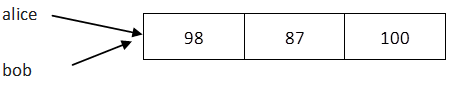
\includegraphics[scale=.6]{alice_bob_same}\\
\end{figure}

When \textit{alice} was modified, \textit{bob} was also modified\\

\begin{figure}[h]
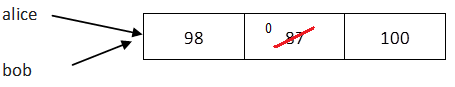
\includegraphics[scale=.81]{alice_bob_modified}\\
\end{figure}


\begin{lstlisting}
>>>  bob                                      

[98, 0, 100]

\end{lstlisting}

What if we wanted \textit{bob} to have a different copy of list, one that initially has the same values as \textit{alice} but that is not affected by future changes to \textit{alice}?

\begin{figure}[h]
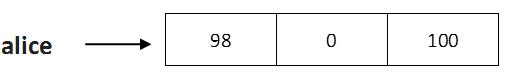
\includegraphics[scale=.545]{alice_different}
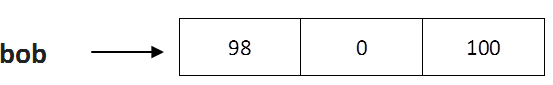
\includegraphics[scale=.5]{bob_different}\\
\end{figure}

If the list we are copying is not nested, the following slice assignment will work.

\begin{lstlisting}
>>> alice = [98, 0, 100]                    

\end{lstlisting}

The two variables \textit{alice} and \textit{bob} point to different locations in memory

\begin{figure}[h]
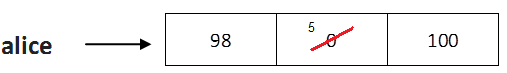
\includegraphics[scale=.745]{alice_different_modified}\\
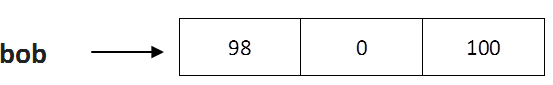
\includegraphics[scale=.51]{bob_different}\\
\end{figure}

\begin{lstlisting}
>>> bob = alice[:]          

\end{lstlisting}

The two variables \textit{alice} and \textit{bob} point to different locations in memory

\begin{lstlisting}
>>> bob

[98, 0, 100]

>>> alice

[98, 0, 100]

>>> alice[1] = 5    

\end{lstlisting}

Only \textit{alice} is modified
\begin{lstlisting}
>>> alice

[98, 5, 100]

\end{lstlisting}

\textit{bob} is unchanged

\begin{lstlisting}
>>> bob

[98, 0, 100]

\end{lstlisting}

However with nested lists the slice assignment will NOT work.  It is a shallow copy.

\begin{figure}[h]
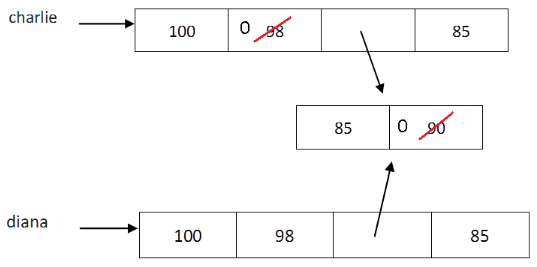
\includegraphics[scale=.745]{charlie}\\
\end{figure}

\begin{lstlisting}
>>> charlie = [100, 98, [85, 90], 85]

>>> diana = charlie[:]

>>> diana

[100, 98, [85, 90], 85]

>>> charlie[1] = 0
\end{lstlisting}

The nested items are shared in the shallow copy

\begin{lstlisting}
>>> charlie

[100, 0, [85, 90], 85]

>>> diana

[100, 98, [85, 90], 85]

>>> charlie[2][1] = 0

>>> charlie

[100, 0, [85, 0], 85]

>>> diana

[100, 98, [85, 0], 85]

\end{lstlisting}

We'll see later on in this course how to use deepcopy to get around this problem.

\subsection{What else can we do with a list?}

If the list items are comparable, we can get their minimum, their maximum and get the list in sorted order.

If the items are numbers, we can also get their sum.

\begin{lstlisting}
>>> grades = [85, 60, 100, 95, 75]

>>> min(grades)

60

>>> max(grades)

100

>>> sum(grades)

415

>>> sorted(grades)

[60, 75, 85, 95, 100]

>>> grades

[85, 60, 100, 95, 75]

\end{lstlisting}

Note that the function sorted does not change the original list.  It returns a sorted copy of the original list.

min, max, sum and sorted are all built-in functions.  We invoke them on a list by specifying the list between the parentheses:  max(grades), min(grades), sum(grades), sorted(grades). Make sure you don't use min, max, sum or sorted as variable names.

There are also many list methods.  We invoke these methods by adding a dot following the method name right after the list as shown below.  We'll cover methods in details later in this course.

\begin{lstlisting}
>>> grades = [85, 60, 100, 95, 75]

\end{lstlisting}

append is a list method that adds a new element to the end of a list.

\begin{lstlisting}
>>> grades.append(100)

>>> grades

[85, 60, 100, 95, 75, 100]

\end{lstlisting}

reverse rearranges the elements in reverse order.

\begin{lstlisting}
>>> grades.reverse()

>>> grades

[100, 75, 95, 100, 60, 85]

\end{lstlisting}

sort rearranges the elements in ascending order.

\begin{lstlisting}
>>> grades.sort()

>>> grades

[60, 75, 85, 95, 100, 100]

\end{lstlisting}

insert  adds an element at a given index position.  To insert 90 at index position 0, we write:

\begin{lstlisting}
>>> grades.insert(0, 90)

>>> grades

[90, 60, 75, 85, 95, 100, 100]

\end{lstlisting}

Note that all these methods (append, reverse, sort and insert) change the original list.

index returns the position of the first occurrence of the given element. 

\begin{lstlisting}
>>> grades.index(75)

2
\end{lstlisting}

count returns the number of occurrences of the given element. 

\begin{lstlisting}
>>> grades.count(100)

2

\end{lstlisting}

We can also remove items from a list:

If we know the index of the element we want, we can use pop: it modifies the list and returns the element that was removed.

\begin{lstlisting}
>>> grades.pop(2)

75

>>> grades

[90, 60, 85, 95, 100, 100]

\end{lstlisting}

75 is no longer an item in grades.

If we don’t provide an index, pop deletes and returns the last element.

\begin{lstlisting}
>>> grades.pop()

100

>>> grades

[90, 60, 85, 95, 100]

\end{lstlisting}

If we know the element we want to remove but not the index, we can use remove:

\begin{lstlisting}
>>> grades.remove(85)

>>> grades

[90, 60, 95, 100]

\end{lstlisting}

Note that only the \textit{first} instance of the given element is removed.

\begin{lstlisting}
>>> grades = [90, 60, 85, 100, 95, 100]

>>> grades.remove(100)

>>> grades

[90, 60, 85, 95, 100]

\end{lstlisting}

extend is a list method that adds ALL the items of a a new list to the end of the current list.

\begin{lstlisting}
>>> grades = [90, 60, 85, 95, 100]

>>> grades.extend([70, 75])

>>> grades

[90, 60, 85, 95, 100, 70, 75]

\end{lstlisting}

We have to specify a list between the parentheses.  The original list grades has been modified. 

Note that writing:

\begin{lstlisting}
grades.extend([70, 75])
\end{lstlisting}

has the same effect as writing:

\begin{lstlisting}
grades = grades + [70, 75]
\end{lstlisting}

or:
\begin{lstlisting}
grades += [70, 75]
\end{lstlisting}

\subsubsection{Extend or append?}

extend adds all the items in the list: 

\begin{lstlisting}
>>> grades = [90, 60, 85, 95, 100]

>>> grades.extend([70, 75])

>>> grades

[90, 60, 85, 95, 100, 70, 75]

\end{lstlisting}

append adds the list as one (nested) item:

\begin{lstlisting}
>>> grades = [90, 60, 85, 95, 100]

>>> grades.append([70, 75])

>>> grades

[90, 60, 85, 95, 100, [70, 75]]

\end{lstlisting}

\subsection{From strings to lists...and back}

Sometimes it is useful to be able to separate some text into a list of words.

The \textbf{split} method allows us to do just that.  It is a string method, so we invoke it on a string and it returns a list of the words in the string.

Let's see how it works with an example:

\begin{lstlisting}
>>>phrase = 'Simple is better than complex'

>>>words = phrase.split()

>>>print(words)

['Simple', 'is', 'better', 'than', 'complex']

\end{lstlisting}

split also allows us to specify a delimiter other than whitespace.

For example we can specify '*' as the delimiter for the split:

\begin{lstlisting}
>>>volume = 'height*weight*depth'

>>>dimensions = volume.split('*')

>>>print(dimensions)

['height', 'weight', 'depth']
\end{lstlisting}

When we don't specify any delimiter, split uses whitespace as the default delimiter.

Whitespace includes the space character ' ', the new line character and the tab character.

It is best to let split default rather than specify one space character as the delimiter.  There are two reasons for that:
\begin{itemize}
\item The default will  work on any whitespace, not just the space character ' '.
\item The default will work when we have more than one space character in a row.
\end{itemize}
  
Consider the following string with two space characters between Hello and World.

\begin{lstlisting}
>>>phrase = 'Hello  World'

>>> extra_words = phrase.split(' ')  

>>> print(extra_words)

['Hello', '', 'World']

>>> words = phrase.split()

>>> print(words)

['Hello', 'World']

\end{lstlisting}

The join method allows us to go back from a list to a single string.  It joins the elements of a list into a string with each element separated by the string that join was invoked on. 

\begin{lstlisting}
>>> words = ['Simple', 'is', 'better', 'than', 'complex']

>>>new_phrase = '*'.join(words)

>>>print(new_phrase)

Simple*is*better*than*complex

\end{lstlisting}

We can also invoke the join method on a single space character:

\begin{lstlisting}
>>>newer_phrase = ' '.join(words)

>>>print(newer_phrase)

Simple is better than complex
\end{lstlisting}

\section{Loops}

\subsection{Range}

Now is a good time to introduce a useful construct in Python.  The range sequence type provides us with a sequence of integers.  We can use this sequence in the for loop, as we would a list.

Note that in Python 2, range was a built-in function that was used to create and return a list.

In Python 3, it returns a range object.

range(3) -> 0, 1, 2 

range of integers from 0 up to but NOT including 3.

\begin{lstlisting}
for i in range(3):
    print(i)
 
0
1
2
\end{lstlisting}

range(1, 5) -> 1, 2, 3 ,4 

range of integers from 1 up to but NOT including 5.

\begin{lstlisting}
for i in range(1, 5):
    print(i)
 
1
2
3
4
\end{lstlisting}

range(5, 52, 5) -> 5, 10, 15, 20, 25, 30, 35, 40, 45, 50 

range of integers from 5 up to but NOT including 52, incrementing by 5 each time.

\begin{lstlisting}
for i in range(5, 52, 5):
    print(i)
 
5
10
15
20
25
30
35
40
45
50

\end{lstlisting}

The integers don't have to be positive:

range (-10, -5) -> -10, -9, -8, -7, -6

\begin{lstlisting}
for i in range(-10, -5):
    print(i)
 
-10
-9
-8
-7
-6

\end{lstlisting}

range (5, -5,-2) -> 5, 3, 1, -1, -3

range of integers from 5 to -5 but NOT including -5, incrementing by -2 each time.

\begin{lstlisting}
for i in range(5, -5, -2):
    print(i)
 
5
3
1
-1
-3

\end{lstlisting}

range(2, -2, 1) -> nothing

range of integers from 2 to -2 but NOT including -2, incrementing by 1 each time.

\begin{lstlisting}
for i in range(2, -2, 1):
    print(i)
 
\end{lstlisting}
 
In general:

range(stop) -> Generates a sequence of integers from 0 up to but not including stop.

range(start, stop) -> Generates a sequence of integers from start up to but not including stop.

range(start, stop, step) -> Generates a sequence of integers from start up to but not including stop incrementing by step.

Note that start, stop and step have to be integers. 

We can also test for membership in a range:

\begin{lstlisting}
>>> pick = 9

>>> pick in range(10)

True

>>> pick in range(5)

False

>>> 5 in range(5)

False

\end{lstlisting}

\section{Functions}
\subsection{What is a function?}

A function is a named sequence of statements.

When we define a function, we specify its name and the sequence of statements. Later, we can call the function by name and the sequence of statements gets executed.

In other words a function is a block of code that is defined once and is executed every time we call it.

We have already seen several  examples of function calls:

\begin{itemize}

\item print('Hello')
\item type(8) 
\item len('Python')
\item int(9.2)
\item str(2015) 
\item min(grades)
\item max(grades)
\item sorted(grades)
\item sum(grades)
\end{itemize}

We say that a function takes an argument and returns a result. The result is called the return value.

Here the function \textit{len} takes a string as its argument and returns the number of characters in the string.

len('Hello') -> 5

'Hello' is the argument and 5 is the return value.

\subsubsection{DRY - Don't Repeat Yourself}


The DRY principle is a central idea in software development.

You should not have multiple fragments of code that perform the same thing – even if you can copy and paste the code into different locations.  That results in code that is harder to test and harder to maintain.

Instead, that logic should be implemented once, given a name, and called multiple times.

\subsection{Function Definition}

To create our own function, we write a function definition.

A function definition starts with the reserved word \textit{def} (short for define), followed by the function name.

Here's a function definition for a function named area:

\begin{lstlisting}
def area(length, width):
    """
    Compute the area of a rectangle
 
    Parameters:
    length, width (float)
    Returns:
    area (float)
    """
    result = length * width
    return result
    
\end{lstlisting}
       
Function names are usually lowercase.  The function name here is area.

Our function takes two input parameters: length and width.  They are placed between parentheses after the function name.  

The function definition header ends with a colon.

Everything in a function  definition is indented. The first line that is not indented is outside the function.  There are no curly braces and no begins and ends to delimit the function otherwise.

A function has its own docstring.  It is the first thing within the function definition.  It is also indented.

\textit{result} is a variable that is local to the function.

A function may or may not have a return statement. The return statement causes the function to exit, and may or may not pass back an expression (return value) to the caller. 

Our function returns the value of the variable result which is the product of the length and width.

If the return statement is omitted the function is exited at the end of the indented code and the value None is returned. The value None is also returned when a return statement is included without an associated expression as in:

\begin{lstlisting}
return
\end{lstlisting}

It is sometimes useful to think of a function as a black box:

\begin{figure}[h]
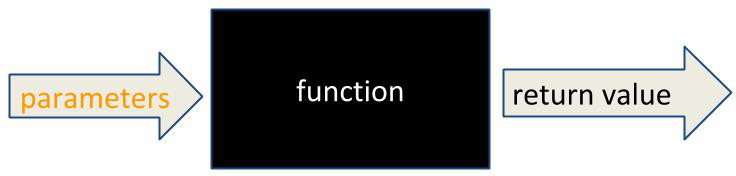
\includegraphics[scale=.5]{blackbox.jpg}\\
\end{figure}

\subsection{Function Calls}

Once we define our function, we can ask it  a question by calling it.  The function responds by returning a value.

Going back to our function area, we can call it with different values for the parameters length and width as follows: 

\begin{lstlisting}
bedroom = area(11, 9)  # first function call
kitchen = area(12, 7)  # second function call
family = area(12, 12)  # third function call
print(bedroom, kitchen, family) 
99 84 144

\end{lstlisting}

The initial values given to the parameters at the point of call are called the arguments.

In the first function call above,  11 and 9  are the arguments to our function.  They define the value that will be assigned to the parameters, length and width inside the function definition.

In the second function call,  12 and 7  are the arguments and in the third function call 12 and 12 are the arguments.

The return value of a given function is accessed by writing function{\_}name(arguments).

To access the return value of the function area when it is called with arguments 11 and 9, I can write area(11, 9).  The corresponding value is 99. 

Note that a return statement is not a print statement.  Just because a value is returned does not mean it will be printed.  If we need the value to be printed, we'll add a print statement as in:

\begin{lstlisting}
print(bedroom, kitchen, family)
\end{lstlisting}

We can also write:

\begin{lstlisting}
print(area(11, 9), area(12, 7), area(12, 12)) 
\end{lstlisting}

We call this function composition:  we are directly using the return value from one function (area) as an input argument to another function (print).

We have already done this in statements such as:

\begin{lstlisting}
print(len(name))

print(max(grades))
\end{lstlisting}

\subsection{Arguments and Parameters}

We've seen that parameters are the variables in the function definition and arguments are the values given to the variables at the point of call.

\textbf{Parameters appear in the function definition; arguments appear in the function calls.}

In Python, we can call a function using one of the following types of arguments:

\begin{itemize}
\item Required positional arguments
\item Keyword arguments
\item Default arguments (positional or keyword)
\end{itemize}

\subsubsection{Required positional arguments}
Required positional arguments are the arguments passed to a function in correct positional order. The number of arguments in the function call should match exactly the number of parameters in the function definition.  

Let's go back to our area function definition and call our function area with different arguments:

\begin{lstlisting}
def area(length, width):
    """
    Compute the area of a rectangle
 
    Parameters:
    length, width (float)
    Returns:
    area (float)
    """
    result = length * width
    return result
 
print(area(8, 3))    
24
 
print(area(4*3, 1+2))
36
 
my_length = 7
print(area(my_length, 2))
14
 
print(area(2))
Traceback (most recent call last):
    print(area(2))
TypeError: area() missing 1 required positional argument: 'width'
\end{lstlisting}

Here we provided one argument instead of two so we got a TypeError.

\begin{lstlisting}
print(area(6, 2, 3))
Traceback (most recent call last):
    print(area(6, 2, 3))
TypeError: area() takes 2 positional arguments but 3 were given
\end{lstlisting}

Here we provided three arguments instead of two so we also got a TypeError.

\subsubsection{Keyword Arguments}

We can also call a function using keyword arguments of the form "keyword=value". We just have to identify the arguments by the parameter name.

This allows us to  skip arguments or place them out of order because the interpreter is able to use the keywords provided to match the values with parameters. 

Let's go back to our area function definition and make sense of this with an example:

\begin{lstlisting}
print(area(5, 2))    
10
 
print(area(length=5, width=2))    
10
 
print(area(width=2, length=5))    
10
\end{lstlisting}

The order of the arguments does not matter because the arguments are matched with the parameter names. 
 
Note however that keyword arguments have to be specified AFTER non-keyword arguments.
\\
\begin{lstlisting}
print(area (length=5,  2)) 
SyntaxError: non-keyword arg after keyword arg
\end{lstlisting}

No argument must receive a value more than once.
\begin{lstlisting}
print(area (2, length=5)) 
TypeError: area() got multiple values for argument 'length'
\end{lstlisting}

Since length is listed before width in the function definition, 2 is assumed to be the length so we end up with multiple values for length.

\subsubsection{Default Arguments}

When we define a function, we can provide default values for its arguments.

When calling that function, arguments with default values are optional. If they are not provided, then the default value is used instead.

Let's define  a new function definition that provides a default value for an argument.  \textbf{Non-default parameters must appear before default parameters in the function definition.} 

The function \textit{diff} below is a valid function definition.  The non-default parameter, first, appears before the default parameter, second.  
 
\begin{lstlisting}
def diff(first, second=0):
    result = first - second 
    return result 
\end{lstlisting}

Now consider the following invalid function definition.  \textit{b} is a non-default parameter and it appears after default parameter a.  This results in a syntax error.

\begin{lstlisting}
def invalid(a=10, b ):
    result = a - b 
    return result 
SyntaxError: non-default argument follows default argument
\end{lstlisting}

Once we have specified the default parameters in the function definition, we can omit the corresponding arguments in the function call.  The default value will be used.

\begin{lstlisting}
print(diff(4))
4
 
print(diff(first=6))
6
 
print(diff(4, 2))
2
 
print(diff(second=3, first=10))
7
 
print(diff(second=3))
Traceback (most recent call last):
  File "C:/...", line ..., in <module>
    print(diff(second = 3))
TypeError: diff() missing 1 required positional argument: 'first'
\end{lstlisting}
 
\textbf{Warning:
Do NOT use a default value for a mutable object such as a list.  This results in unexpected behavior.}

Consider the following code:

\begin{lstlisting}
def add_one(a_list):
    a_list.append(1)    #  append item 1 to the given list
    return a_list
 
first_list = add_one([])      # [] denotes the empty list
print(first_list)
second_list = add_one([])
print(second_list)
third_list = add_one([])
print(third_list)
[1]
[1]
[1]
\end{lstlisting}

If instead of calling add{\_}one and specifying [] as the argument, I decide to specify a default parameter for add{\_}one in the function definition as follows. I would expect the same result, but I get something different.

\begin{lstlisting}
def add_one(a_list=[]):
    a_list.append(1)
    return a_list
 
first_list = add_one()         # use the default value
print(first_list)
second_list = add_one()    # use the default value
print(second_list)
third_list = add_one()       # use the default value
print(third_list)
[1]
[1, 1]
[1, 1, 1]
\end{lstlisting}

The reason for this behavior is that Python evaluates the default argument once, when the def statement is executed  and the same list (now modified) keeps being used.  This may result in some hard to find bugs.
To be safe, avoid it completely or use the following: 

\begin{lstlisting}
def add_one(a_list=None):
    if a_list == None:
        a_list = []
    a_list.append(1)
    return a_list
\end{lstlisting}
 
\subsubsection{Example: Print Function Arguments}

The print function has optional parameters \textit{sep} and \textit{end}.  We can use the keyword arguments to bypass the default.

\textit{sep} defaults to a space character ' '.

\textit{end} defaults to new line.\\ 

If we want to specify a different separator, we specify it as follows:

\begin{lstlisting}
print ('Hello', 'World', sep='|')

Hello|World

\end{lstlisting}

If we don't want a new line between print functions calls, we use:

\begin{lstlisting}
print('Hello', end=' ')

print('World', end=' ')

Hello World

\end{lstlisting}

In summary:
\begin{itemize}
\item The positional arguments always go first, followed by any keyword arguments.

\item The keywords must be chosen from the formal parameter names.

\item No argument must receive a value more than once. 
\end{itemize}

\subsection{What's in a Name?}

Let's take a minute to talk about naming rules for identifiers in Python.  An identifier may be a variable name, a function name, a parameter name and so on.

Identifier names are case sensitive.  \textit{grade} and \textit{Grade} are not the same.

Identifiers must begin with a letter or an underscore.  Subsequent characters can be letters, digits or underscores.  \textit{grade}, \textit{Grade1}, \textit{homework{\_}grade} and \textit{{\_}grade} are all valid identifiers. However, \textit{1grade} and \textit{grade{\#}1} are NOT.


An identifier  cannot be a reserved word.  Reserved words are words that have a special meaning in Python such as \textit{True}, \textit{False} and \textit{else}.  
The rules above are the syntax rules.  

However for readability,  we have a number of style rules in Python. The \href{https://www.python.org/dev/peps/pep-0008/}{Style Guide for Python} has the following style guidelines.  We'll follow these closely in this course:

\begin{itemize}
\item Function names should be lowercase, with words separated by underscores. Descriptive names are encouraged.
Example: area, compute{\_}grade

\item Function names typically describe operations applied to arguments by the interpreter (like print, add) or the name of the quantity that results (like max, sum).
Variable names should also be lowercase, with words separated by underscores as necessary to improve readability.
Example: homework{\_}grade,  final{\_}grade

\item Parameter names should be lowercase, with words separated by underscores. Single-word names are preferred.
Parameter names should describe the role of the parameter in the function, not just the type of value that is allowed.
Never use "l" (lowercase ell), "O" (capital oh), or "I" (capital i) to avoid confusion with numerals. 
\end{itemize}

\subsection{Functions and Variable Scope}

The scope of an identifier refers to the part of the program where that identifier is visible, where it can be accessed.

Because variables are not declared ahead of time, Python uses the location of the assignment to associate a variable with a scope. The place where you assign a variable in your code determines its scope of visibility.

The variables defined inside a function definition can only be seen by the code in that function definition.  We cannot refer to these variables from outside the function.


Order does matter.  We can only access (read) a variable in our scope after it has been assigned a value.  The scope of a variable in a function extends from the assignment statement until the end of the function.  It does not include code that came before the assignment statement.
The parameters defined inside a function definition can be seen by the code in that function definition.  The only other place that we can refer to them is in the function call (as keyword arguments. 

Variables defined inside one function definition do not conflict with variables defined in other function definitions.  The same name may be used in different functions.
 
Let's take a look at a few examples to clarify scope:

\begin{lstlisting}
def multiply(number):
    factor = 5
    result = factor * number
    print(factor)
    return result
 
answer = multiply(10)

\end{lstlisting}
 
The corresponding output is: 5
 
The variable factor may be accessed from inside the function \textit{multiply}. However if we move the print statement to outside the function, thus outside the variable scope, we get a NameError:

\begin{lstlisting} 
def multiply(number):
    factor = 5
    result = factor * number
    return result
 
answer = multiply(10)
print(factor)
 
NameError: name 'factor' is not defined
\end{lstlisting}
 
If we move the print statement inside the function, but before the assignment statement we also get a NameError.  Order matters: the print statement is no longer in the scope.

\begin{lstlisting} 
def multiply(number):
    print(factor)
    factor = 5
    result = factor * number
    return result
 
answer = multiply(10)
 
NameError: name 'factor' is not defined
\end{lstlisting}
 
We can use the keyword parameter \textit{number} outside the function definition:

\begin{lstlisting} 
def multiply(number):
    factor = 5
    result = factor * number
    return result
 
answer = multiply(number=10)
print(answer)
\end{lstlisting}
 
The corresponding output is: 50
 
However we cannot access the parameter number outside the function definition and outside the function call:

\begin{lstlisting} 
def multiply(number):
    factor = 5
    result = factor * number
    return result
 
answer = multiply(10)
print(number)
 
NameError: name 'number' is not defined
\end{lstlisting}
 
The same variable name may be used in different functions.  

\begin{lstlisting}
def multiply(number):
    factor = 5
    result = factor * number
    return result
 
def half(number):
    result = number / 2
    return result
    
first = multiply(10)
second = half(10)
print(first, second)
50, 5.0
\end{lstlisting}

There is no conflict here, the two variables have different scopes.

\subsection{Pure Functions and Side Effects}

Pure functions are supposed to take an input and return a result with no side effects.  The function area that we defined earlier is a pure function.

By contrast, consider the following function:
\begin{lstlisting}
def double(n):
    print(n)
    result = 2 * n
    return result
\end{lstlisting}
    
double takes an input and returns a result (2*n) but it also causes something to be printed. 

Sometimes the side effect is not obvious.  Consider the following function:

\begin{lstlisting}
def special_surface(a_list):
    """
    return the product of the first two elements of the list.
    if one of the elements is 0, return the other.
    """
    if a_list[0] == 0:
        a_list[0] = 1       
    elif a_list[1] == 0:
        a_list[1] = 1
    result = a_list[0] * a_list[1]
    return result

dimensions = [10, 0, 20]
print('dimensions before the function call: ', dimensions)
answer = special_surface(dimensions)
print(answer)
print('dimensions after the function call: ', dimensions)
\end{lstlisting}

The output from the lines of code above is:

\begin{lstlisting}
dimensions before the function call:  [10, 0, 20]
10
dimensions after the function call:  [10, 1, 20]
\end{lstlisting}
 
The function call returns the right product, but it has changed the original list!
Note that this is mainly due to the fact that the argument is a list and lists are mutable.  

To avoid the side effect, we redefine our function:

\begin{lstlisting}
def special_surface(a_list):
    """
    return the product of the first two elements of the list.
    if one of the elements is 0, return the other.
    """
    if a_list[0] == 0:
        result = a_list[1]
    elif a_list[1] == 0:
        result = a_list[0]
    else:
        result = a_list[0] * a_list[1]
    return result
       
dimensions = [10, 0, 20]
print('dimensions before the function call: ', dimensions)
answer = special_surface(dimensions)
print(answer)
print('dimensions after the function call: ', dimensions) 
\end{lstlisting}

Now the output is:

dimensions before the function call:  [10, 0, 20]
10
dimensions after the function call:  [10, 0, 20]
 
Side effects such as this are often the source of bugs in our programs.  It is best to avoid them when possible.

\subsection{The Main Function}

Now that we know how to define our own functions, we're ready to place all our Python statements inside functions.  We'll be following this programming practice from here on in this course.

We'll place the main part of the code (the part that did not fall into a function but was used to call the other functions and possibly print the results) into a function that we'll call, well, \textit{main}.  

Going back to our area example, instead of:

\begin{lstlisting}
def area(length, width):
    """
    Compute the area of a rectangle
 
    Parameters:
    length, width (float)
    Returns:
    area (float)
    """
    result = length * width
    return result    
 
bedroom = area(11, 9)  # first function call
kitchen = area(12, 7)  # second function call
family = area(12, 12)  # third function call
print(bedroom, kitchen, family) 
\end{lstlisting}
 
We'll write:

\begin{lstlisting} 
def area(length, width):
    """
    Compute the area of a rectangle
 
    Parameters:
    length, width (float)
    Returns:
    area (float)
    """
    result = length * width
    return result  
 
def main():
    bedroom = area(11, 9)  # first function call
    kitchen = area(12, 7)  # second function call
    family = area(12, 12)  # third function call
    print(bedroom, kitchen, family)
\end{lstlisting}    
    
In this case our main function takes no arguments and returns no value.  

However, if you save this program in PyCharm and try to run it, you'll notice that no output is generated.  No statement is executed either.  \textbf{Function definitions don't execute any code without any function calls.}  The function calls to area are inside the main function, however there is no function call to main.

To fix that, we add the function call: main()

\begin{lstlisting}
def area(length, width):
    """
    Compute the area of a rectangle
 
    Parameters:
    length, width (float)
    Returns:
    area (float)
    """
    result = length * width
    return result  
 
def main():
    bedroom = area(11, 9)  # first function call
    kitchen = area(12, 7)  # second function call
    family = area(12, 12)  # third function call
    print(bedroom, kitchen, family)
 
main()
\end{lstlisting}

\subsection{Python Module}

A Python module is basically a file that contains Python code.  

The module name is the file name without the extension.

For example, when the file name is house.py, the corresponding module name is house.  

Let's  take a look at the following Python module.

\begin{lstlisting}
# -----------------------------------------------------------------------------
# Name:        house
# Purpose:     demonstrate the structure of a Python module
# Author:      Rula Khayrallah
# Created:     1/18/2015
# -----------------------------------------------------------------------------
"""
Compute and print the area of different rooms in a house

Compute the area of the kitchen, bedroom and family room in square feet.
Print the three areas in square feet.
"""
def area(length, width):
    """
    Compute the area of a rectangle

    Parameters:
    length, width (float)
    Returns:
    area (float)
    """
    result = length * width
    return result

def main():
    bedroom = area(11, 9)
    kitchen = area(12, 7)
    family = area(12, 12)
    print(bedroom, kitchen, family)

if __name__ == '__main__':
    main()
\end{lstlisting}
 
This is our module house in the file house.py.

The file starts with block comments that include information such as author and date.

The module itself has a docstring documenting its use.

Then we have the area function definition with its own docstring and function body.

Note that a given module may contain several function definitions.

Then comes the main function which calls the area function three times and uses the return values to produce some output.

Finally we have added the condition \textit{if {\_}{\_}name{\_}{\_} == '{\_}{\_}main{\_}{\_}':}  before the call to main, outside any function.

This is to allow the module to be  imported and have its functions, classes or definitions used by some other module.  

When a module is run directly, the special variable "{\_}{\_}name{\_}{\_}" is set to "{\_}{\_}main{\_}{\_}".   In this case, the main function will be executed.  

However when the module is imported the function main will not be executed.  We'll see later how to import a module and use its functions in another module.  

From now on, we'll be adding \textit{if {\_}{\_}name{\_}{\_} == '{\_}{\_}main{\_}{\_}':} as shown above to all our Python files to make them valid modules that can be either run directly or imported.

\subsection{Control Flow}

Let's take a closer look at the order in which the statements are executed in our program.

The comments and docstrings are ignored by the interpreter.   The numbers added as inline comments to the right of the statements reflect the order in which the statements are executed. 

\begin{lstlisting}
# -----------------------------------------------------------------------------
# Name:        house
# Purpose:     demonstrate the structure of a Python module
# Author:      Rula Khayrallah
# Created:     1/18/2015
# -----------------------------------------------------------------------------
"""
Compute and print the area of different rooms in a house

Compute the area of the kitchen, bedroom and family room in square feet.
Print the three areas in square feet.
"""
def area(length, width):
    """
    Compute the area of a rectangle

    Parameters:
    length, width (float)
    Returns:
    area (float)
    """
    result = length * width   # 4 8 12
    return result             # 5 9 13

def main():
    bedroom = area(11, 9)     # 3 6
    kitchen = area(12, 7)     # 7 10
    family = area(12, 12)     # 11 14
    print(bedroom, kitchen, family)  # 15

if __name__ == '__main__':    # 1
    main()                    # 2
\end{lstlisting}
 
The statements are executed from top to bottom, so the interpreter encounters the function definitions first.  However the statements inside the function definition are NOT executed until the function is called.

So we get to the unindented statement: \textit{if {\_}{\_}name{\_}{\_} == '{\_}{\_}main{\_}{\_}':}

This is the only statement in our module that is not inside a function, and that is what is executed first.  When we run the program from PyCharm or from the terminal, the value of the special variable {\_}{\_}name{\_}{\_} is set to '{\_}{\_}main{\_}{\_}'  so the condition for the if statement is True and the indented statement main() is executed.

So we go to the function main and execute its statements one after the other.

\textit{main} in turn calls area with the arguments 11 and 9 so we go to area and execute its statements in order.  When we get to the return statement of area, control goes back to main and the return value is saved in the variable bedroom.  That is why the statement  \textit{bedroom = area(11, 9)}  has two numbers 3 and 6.

Then we go on to the next statement in main:   \textit{bedroom = area(12, 7)}.  Here, \textit{area} is called again but with the arguments 12 and 7.  The statements inside \textit{area} are now executed again.  When we get to the return statement of \textit{area}, control goes back to main and the return value is saved in the variable kitchen.

Then we go on to the next statement in main:   family = area(12, 12).  area is called again but with the arguments 12 and 12.  The statements inside area are now executed again.  When we get to the return statement of area, control goes back to main and the return value is saved in the variable family.

After that we print the three variables (statement 15) and we're done.

Note that in this simple example, there are no loops so it is straightforward to assign numbers to each statement. That will not be possible in more complex code where the control flow may depend on user input.

To visualize the program execution we can use the Python visualizer available  at http://pythontutor.com/  or the PyCharm debugger.

\subsection{Global Variables?}

Variables defined in the outer statements outside any function are called global variables.

We'll examine how global variables work in Python but we'll avoid using them in our programs because they result in code that is less readable, harder to debug and more difficult to maintain.

Constants defined in the outer statements outside any function are called global constants.  These are OK to use as long as we only read them and not modify them inside the functions.  Global constants are especially useful  when the same constant is used in several functions.

Example 1:  Global constants are OK
\begin{lstlisting}
"""
Tip calculator assuming a 20% tip rate

Prompt the user for the cost of their meal.
Print the tip amount and the total cost.
"""
TIP_RATE = 20/100            # global tip rate constant: 20%
def get_input():
    """
    prompt the user for the cost of their meal

    parameter: none
    returns:the user input as a float
    """
    user_input = input('Please enter the cost of your meal in $: ')
    number = float(user_input)  # convert the input string to a number
    return number

def get_tip(amount):
    """
    compute the tip corresponding to the given amount

    parameter: amount (float)
    returns:the 20% tip rounded to 2 decimals
    """
    result = TIP_RATE * amount   # calculate the tip amount
    result = round(result, 2)    # round the tip to two decimals
    return result

def total(first, second):
    """
    Compute the sum of two amounts rounded to 2 decimals

    parameters: first, second (floats)
    returns: the sum rounded to 2 decimals
    """
    result = first + second
    result = round(result, 2)
    return result

def main():
    cost = get_input()
    tip = get_tip(cost)
    print('Tip Amount: $', tip, sep='')
    pay = total(cost, tip)
    print('Total amount to pay: $', pay, sep='')

if __name__ == '__main__':
    main()
 
Please enter the cost of your meal in $: 20
Tip Amount: $4.0
Total amount to pay: $24.0
\end{lstlisting}

Example 2:  Avoid global variables

\begin{lstlisting} 
count = 0 # global variable - bad practice

def count_by_two():
    global count
    count = count + 2
    return

def main():
    for i in range(5):
        count_by_two()
        print(count)
 
2
4
6
8
10
\end{lstlisting}

 Note that because the variable count is assigned in the global scope (that is in the outermost code), the function main has read access to it: print(count) in main does not generate any error.
However in order to modify the variable count, the function count{\_}by{\_}two has to include the statement:

global count

That global statement is required to signal that the following assignment statement is modifying a global variable and not creating a new local variable.

Example 3:  Use parameters and return values  instead of global variables to communicate between functions
 
\begin{lstlisting}
def count_by_two(count):
    result = count + 2
    return result

def main():
    main_count = 0
    for i in range(5):
        main_count = count_by_two(main_count)
        print(main_count)
 
2
4
6
8
10
\end{lstlisting}

\subsection{Lambda Functions}

Anonymous functions in Python are called \textit{lambda functions}.

Lambda functions offer a concise way to define functions without giving them a name.  They are used to create and use functions on the fly.  Lambda functions are usually passed as arguments to other functions.  We'll see several examples of lambda function use later in this course.

The syntax to specify a lambda function is as follows:

\begin{lstlisting}
lambda parameters: return_value
\end{lstlisting}

The above is a Python expression.  It can appear in an assignment statement or as an argument to another function.

Let's look at examples of valid lambda functions in Python:

\begin{lstlisting}
lambda x: x ** 2
\end{lstlisting}

We can use the lambda above in the assignment statement:

\begin{lstlisting}
square = lambda x: x ** 2
\end{lstlisting}

Now the variable square is a function.  
\\
\begin{lstlisting}
>>> square(5)

25
\end{lstlisting}

The above is equivalent to the following:

\begin{lstlisting}
def square(x):

    return x ** 2
\end{lstlisting}

Here's another lambda function:

\begin{lstlisting}
lambda word: word.lower()
\end{lstlisting}

We can use the lambda above in the assignment statement:

\begin{lstlisting}
f  = lambda word: word.lower()
\end{lstlisting}

Now the variable f is a function.

\begin{lstlisting}
>>> f('HELLO')

'hello'
\end{lstlisting}

The above is equivalent to the following function definition:

\begin{lstlisting}
define f(word):

    return word.lower()
\end{lstlisting}

Here's a lambda function that takes two parameters:

\begin{lstlisting}
lambda a, b: a + b

add = lambda a, b: a + b
\end{lstlisting}

The above is equivalent to the following function definition:

\begin{lstlisting}
def add(a, b):

    return a + b
\end{lstlisting}

\section{Recursive Functions}
\subsection{Recursion}

We use recursion when we have a large problem that can be repeatedly broken down into one or more sub-problems.  

To illustrate the process,  we'll go back to our factorial example from module 4 and implement it using a recursive approach.

The factorial of a non-negative integer (!) is the product of all the integers from 1 up to and including the given integer.

By convention, the factorial of 0 is 1.

\begin{itemize}

\item 0! = 1

\item 1! = 1 = 1

\item 2! = 2 * 1 = 2

\item 3! = 3 * 2 * 1 = 6

\item 4! = 4 * 3 * 2 * 1 = 24

\item 5! = 5 * 4 * 3 * 2 * 1 = 120
\end{itemize}

If we look closely at the above, we note that:
\begin{itemize}

\item 5! = 5 * 4!

\item 4!  = 4 * 3!

\item 3! = 3 * 2!

\item 2! = 2 * 1!

\item 1! = 1 * 0!

\item 0! = 1
\end{itemize}

Now let's write a Python function fact that will compute the factorial of a given number.  We'll call our function \textit{fact}.

We know that:
\begin{itemize}
\item fact(5) = 5 * fact(4) 
\item fact(4) = 4 * fact(3) 
\item fact(3) = 3 * fact(2) 
\item fact(2) = 2 * fact(1) 
\item fact(1)= 1 * fact(0) 
\item fact(0) = 1
\end{itemize}
 

In general for a given positive integer n:

\textbf{fact(n) = n * fact(n - 1)}

This is known as the recursive rule: it is the rule by which we express the problem in terms of one or more smaller sub-problems.  The smaller sub-problem here is computing the factorial of n - 1.  To solve the smaller sub-problem, the function calls itself with a smaller argument. 

Eventually the function will come across a sub-problem that is small enough so that it can handle it without calling itself.   This is known as the \textit{base case}.  Our base case here is fact(0).  We know that: fact(0) = 1.

In the base case, the problem-size is as small as it can be.

The base case is needed to prevent the function from calling itself over and over again without stopping: the base case stops the recursion.

In the base case, the function knows the result or can compute it using some straightforward formula.

Now we are ready to write the following recursive definition of our factorial function:

\begin{lstlisting}
def fact(number):
    """ compute the factorial of a non-negative integer """
    # base case: the problem-size is as small as it can be
    if number == 0:
        return 1
    else:
        # recursive rule: the function calls itself with a smaller argument
        return number * fact(number - 1)
\end{lstlisting}
          
The general structure of a recursive function is as follows:

\begin{lstlisting}
def recursive_function(problem):
    if base case condition:
        return base case result
    else: # recursive rule
        return some result that involves recursive_function(sub_problem)
\end{lstlisting}

\subsection{Fibonacci Numbers Example}

For a more complex recursive example, we'll examine Fibonacci numbers.  Fibonacci numbers appear in several mathematical areas.  We'll take a look at one illustration that describes the growth of a rabbit population.

First we assume that a newly born pair of rabbits is put in a field. At the end of its second month a pair of rabbits produces another pair of rabbits.  Rabbits never die and each pair always produces one new pair every month from the second month on.

Our task is to determine how many pairs of rabbits will be in the field in one year.

Let fibonacci(n) denote the number of pairs of rabbits at the start of month n.

fibonacci(0) is 0.

fibonacci(1) is  1 since there is one pair of rabbits at the start of month 1.

Then from month 2 on, the rabbits in the field at the start of month n are:

the same rabbits in the field at the start of month  n - 1 (since rabbits never die)

+ the newborn rabbits.

Since each  each pair of rabbits  produces one new pair every month from their second month on, the number of newborn rabbits at the start of month n is equal to the number of rabbits that are at least 2 months old.

So the number of newborn pairs at the start of month n is equal to the number of pairs of rabbits in the field two months earlier: fibonacci(n - 2).

So we can write:

fibonacci(n) = fibonacci(n - 1) + fibonacci(n-2)

This will be our recursive rule.  Note that in this case, we are formulating the problem in terms of two smaller sub-problems.

Our base case:

fibonacci(0)  = 0 

fibonacci(1)  =  1

\begin{itemize}
\item n	fibonacci(n)
\item 0	0
\item 1	1
\item 2	1 + 0 = 1
\item 3	1 + 1 = 2
\item 4	2 + 1 = 3
\item 5	3 + 2 = 5
\item 6	5 + 3 = 8
\item 7	8 + 5 = 13
\item 8	13 + 8 = 21
\end{itemize}

We can now write our recursive fibonacci function as follows:

\begin{lstlisting}
def fibonacci(n):
    """
    return the Fibonacci number 
    """
    # base case: 0 or 1
    if n <= 1:
        return n
    else:  # recursive rule
        return fibonacci(n-1) + fibonacci(n-2)
\end{lstlisting}
        
We still need to answer the question: how many pairs of rabbits will there be in the field in one year?

In one year, at the beginning of month 13, there will be: fibonacci(13) pairs of rabbits:

\begin{lstlisting}
def main():
    print('In one year, there will be', fibonacci(13), 'pairs of rabbits.')
\end{lstlisting}
    
We get:

In one year, there will be 233 pairs of rabbits.

Note that the recursive implementation above is natural and elegant but not efficient.

The fibonacci function is called 15 times to compute fibonacci(5).  It is called 753 times to compute fibonacci(13).

In Python, the alternate solution using a list and a for loop is much more efficient, but not as elegant:

\begin{lstlisting}
def fibonacci(n):
    """
    return the Fibonacci number  - non recursive solution
    """
    fib = [0,1] # keep a list of the last 2 known fibonacci numbers
    for i in range(2, n+1):
       # calculate fibonacci(i) and append it to the list
        fib.append(fib[-1]+fib[-2]) 
        del fib[0]   # we only need the last two numbers in the sequence
    return fib[-1]  # the last item in the list is fibonacci(n)
\end{lstlisting}

\section{Sequence Data Types}
\subsection{What are they?}
We have already encountered several native data types in Python.  

We have seen numeric data types such as integers, float and complex numbers.  We have discussed booleans.   We have also examined lists and introduced strings and range objects.  These last three, lists, strings and range objects along with some other data types we'll introduce later in this course belong to a special group that is called the 'sequence data types.'

\textbf{A sequence is an ordered collection of data values.}   It has an arbitrary (but finite) number of ordered elements.

The sequence data types all have similar behaviors, and they share some common properties.

We have already seen how to iterate over the items of some sequences with a for loop. 

\begin{lstlisting}
for variable in sequence:
       indented statement(s) 
Other statements…
\end{lstlisting}

Specifically, we have seen how to iterate over the items of a list:

\begin{lstlisting}
cs21 = ['Alice', 'Bob', 'Carol', 'Evan']

for student in cs21:
    print('Hello', student)
print('Welcome to CS21A')
 
Hello Alice
Hello Bob
Hello Carol
Hello Evan
Welcome to CS21A
\end{lstlisting}

We have also seen how to iterate over the characters in a string:

\begin{lstlisting}
phrase = 'Python rules'

for char in phrase:
    print(char)
print(phrase)
\end{lstlisting}

The corresponding output is:\\
 
P\\
y\\
t\\
h\\
o\\
n\\
 
r\\
u\\
l\\
e\\
s\\
Python rules\\
 
Finally, we  have seen how to iterate over the integers in a range:

\begin{lstlisting} 
for number in range(1, 5):
    print(number)
 
1
2
3
4
\end{lstlisting}

We'll take a look at some of the remaining properties shared by sequence data types next.

\subsection{Indexing}

Sequence data types support \textbf{0 based indexing.}  Let's review some examples with lists, strings and range objects.

We can use [] to access the value at a given index position:

\begin{lstlisting}
>>> grades = [100, 85, 90]

>>> phrase = 'Python is fun!'

>>> valid_grades = range(60, 101)

>>> grades[0]

100

>>> grades[-1]

90

>>> phrase[0]
'P'

>>> phrase[-1]

'!'

>>> valid_grades[0]

60

>>> valid_grades[-1]

100
\end{lstlisting}

We can use the method \textit{index} to find the first position of a given element:

\begin{lstlisting}
>>> grades.index(100)

0

>>> phrase.index('n')

5

>>> phrase.index('n', 6)   # what if we start looking at position 6?

12

>>> valid_grades.index(70)

10
\end{lstlisting}

With strings we can also use index to find the first position of a substring:

\begin{lstlisting}
>>> phrase.index('is')

7
\end{lstlisting}

If the element is not found in the sequence, we get a ValueError:

\begin{lstlisting}
>>> grades.index(75)
Traceback (most recent call last):
  File "<input>", line 1, in <module>
ValueError: 75 is not in list
 
>>> phrase.index('a')
Traceback (most recent call last):
  File "<input>", line 1, in <module>
ValueError: substring not found
 
>>> valid_grades.index(50)
Traceback (most recent call last):
  File "<input>", line 1, in <module>
ValueError: 50 is not in range
\end{lstlisting}

Sequence data types support slicing:

\begin{lstlisting}
>>> grades[1:3]
[85, 90]
 
>>> phrase[-4:-1]
'fun'
 
>>> valid_grades[10:20]
range(70, 80)
\end{lstlisting}

\subsection{Membership Test}

We can use 'in' and 'not in' to test for membership in any sequence data type.

We've already seen the membership test in lists:

\begin{lstlisting}
>>> grades = [100, 85, 90]
>>> if 100 in grades:
...     print('Excellent')
...     
Excellent
\end{lstlisting}

The membership test also works with strings:

\begin{lstlisting}
>>> phrase = 'Python is fun!'

>>> 'e'  in phrase

False

>>> '!'  in phrase

True
\end{lstlisting}

And the membership test works with range objects:

\begin{lstlisting}
valid_grades = range(60, 101)
homework = int(input('Please enter the homework grade: '))
if homework not in valid_grades:
     print('Invalid grade entered!')
 
Please enter the homework grade: 30
Invalid grade entered!
Please enter the homework grade: 89
\end{lstlisting}

\subsection{Boolean Interpretation}

The boolean interpretation of an empty sequence is False.

\begin{lstlisting}
>>> empty_list = []

>>> bool(empty_list)

False

>>> bool('')

False

>>> empty_range = range(2, 2)

>>> bool(empty_range)

False
\end{lstlisting}

The boolean interpretation of a non empty sequence is True.

\begin{lstlisting}
grades = [100, 85, 90]

>>> bool(grades)

True

>>> bool('Hello')

True

valid_grades = range(60, 101)

>>> bool(valid_grades)

True
\end{lstlisting}

\subsection{Length and Count}

Sequence data types have a finite length.  We can use the same function \textit{len} to access it:

\begin{lstlisting}
>>> len(grades)

3

>>> len(phrase)

14

>>> len(valid_grades)

41
\end{lstlisting}

Sequence data types also provide a very handy count method that returns the number of occurrences of one element:

\begin{lstlisting}
>>> grades.count(90)

1

>>> phrase.count('n')

2

>>> valid_grades.count(0)

0

>>> zen = 'In the face of ambiguity, refuse the temptation to guess.'

>>> zen.count('e')

7
\end{lstlisting}

\subsection{Minimum and Maximum}

When the elements of a sequence data type are comparable, we can use the functions min and max to get the minimum and maximum element in that sequence.

We have already seen how to use min and max with a list whose elements are numeric:

\begin{lstlisting}
>>> grades = [100, 85, 90]

>>> min(grades)

85

>>> temperatures = [98.4,  95.2, 90]

>>> max(temperatures)

98.4
\end{lstlisting}

We can also use min and max with a list whose elements are strings - strings are compared based on the alphabetical order (it's actually the unicode order).

\begin{lstlisting}
>>> cities = ['San Francisco', 'San Jose', 'Los Angeles', 'San Diego']

>>> min(cities)

'Los Angeles'

>>> max(cities)

'San Jose' 
\end{lstlisting}

We can also use min and max on the sequence data type string because the 'elements' of a string are characters and characters are comparable based on their alphabetical or unicode order.

\begin{lstlisting}
>>> phrase = 'Python is fun!'

>>> max(phrase)

'y'

>>> min(phrase)

' '
\end{lstlisting}

Finally, the elements of a range object are integers and hence they are comparable:

\begin{lstlisting}
>>> valid_grades = range(60, 101)

>>> min(valid_grades)

60

>>> max(valid_grades)

100
\end{lstlisting}

\subsection{More on Strings}

In addition to the common sequence operations, the string data type includes some powerful methods that come in handy in text processing.  

We've seen how to go from a string to a list and back using the split and join methods.

We'll elaborate on the difference between methods and functions when we get to object oriented programming.  For now, we'll note that the syntax to invoke a method is: object{\_}name.method{\_}name().

The method \textit{upper} returns a copy of the string with all the lowercase characters converted to uppercase.  Note that you have to put the () after \textit{upper} to invoke the method on the given string.  

Here's how we use the method \textit{upper} to get an uppercase copy of the original string phrase:

\begin{lstlisting}
>>> phrase = 'Python is fun!' 

>>> upper_phrase = phrase.upper()

>>> print(upper_phrase)

PYTHON IS FUN!

>>> print(phrase)

Python is fun!
\end{lstlisting}

It is a common mistake to assume that because we have invoked upper on a string, it has been modified to contain only uppercase characters.  This is not correct.  \textbf{Strings are immutable}:  the upper method does not change the original string.  It returns an uppercase copy.

Similarly, the method \textit{lower} returns a copy of the string with all the uppercase characters converted to lowercase. 

Here's how we use the method \textit{lower} to get a lowercase copy of the original string phrase:

\begin{lstlisting}
>>> phrase = 'Python is fun!' 

>>> lower_phrase = phrase.lower()

>>> print(lower_phrase)

python is fun!

>>> print(phrase)

Python is fun!
\end{lstlisting}

Here again the \textit{lower} method does not change the original string.  It returns a lowercase copy.

The \textit{strip} method returns a copy of the string with the leading and trailing characters specified removed. 

Let's show how that works with some examples:

\begin{lstlisting}
>>> zen = '   Simple is better than complex.     '
\end{lstlisting}

When we invoke \textit{strip} without specifying an argument as in zen.strip(), the leading and trailing space characters are removed.

\begin{lstlisting}
>>> zen.strip()

'Simple is better than complex.'
\end{lstlisting}

Note that only \textit{leading} and \textit{trailing} space characters are removed. Space characters inside the string (like the one between is and better) are not removed.

We can specify a given character, then this character is removed only if it happens to be at the beginning or end of the string:

\begin{lstlisting}
>>> zen.strip('.')

'   Simple is better than complex.     '

>>> 'Flat is better than nested.'.strip('.')

'Flat is better than nested'
\end{lstlisting}

We can specify more than one character to be removed:

\begin{lstlisting}
>>> zen.strip('. ')    #  period and space character

'Simple is better than complex'
\end{lstlisting}

The \textit{format} method returns a copy of the string where fields delimited by {} are replaced with corresponding values.

\begin{lstlisting}
>>> zen = '{} is better than {}.'

>>> print(zen.format('simple', 'complex'))

simple is better than complex.

>>> print(zen.format('explicit', 'implicit'))

explicit is better than implicit.

>>> print(zen.format('now', 'never'))

now is better than never.
\end{lstlisting}

We can specify a name for the replacement fields.

\begin{lstlisting}
>>> zen = '{first} is better than {second}.'

>>> print(zen.format(first='flat', second='nested'))

flat is better than nested.

>>> print(zen.format(second='complicated', first='complex'))

complex is better than complicated.
\end{lstlisting}

We can specify an index for the replacement fields.

\begin{lstlisting}
>>> zen = '{0} is better than {1}.'

>>> print(zen.format('sparse', 'dense'))

sparse is better than dense.

>>> >>> print('He said: {0} {0} {0}!'.format('HO'))

He said: HO HO HO!
\end{lstlisting}

We can also specify a width:

\begin{lstlisting}
>>> print('Grade: {:6}'.format(100))

Grade:    100

>>> print('Grade: {:6}'.format(85))

Grade:     85

>>> print('Grade: {:6.2f}'.format(100))

Grade: 100.00

>>> print('Grade: {:6.2f}'.format(85.5))

Grade:  85.50
\end{lstlisting}

Some string methods allow us to answer specific questions about a given string.  Here are a few examples:

\begin{lstlisting}
>>> 'Foothill'.isalpha()

True

>>> 'Foothill'.isdigit()

False

>>> '2016'.isdigit()

True

>>> 'Foothill'.startswith('hill')

False

>>> 'Foothill'.endswith('hill')

True
\end{lstlisting}

There are many more methods available on strings in Python.  One way to get a list of these methods is to use code completion in the interpreter shell or the editor.  Typing the string variable name followed by a dot brings up a list of all the methods available on the strings:

String methods: 
\begin{itemize}
\item capitalize() 
\item casefold() 
\item center() 
\item count() 
\item encode() 
\item endswith() 
\item expantabs() 
\item find() 
\item format()
\end{itemize}

There are also some predefined string constants that we can conveniently use in our programs.

To access these constants, we need to add the statement 'import string' to the top of our program, after the docstring,  or if we are at the interpreter prompt, execute it from there.

\begin{lstlisting}
>>> import string  

>>> string.punctuation

'!"#$%&\'()*+,-./:;<=>?@[\\]^_`{|}~' 

>>> string.digits

'0123456789‘

>>> string.ascii_lowercase

'abcdefghijklmnopqrstuvwxyz'

>>> string.ascii_uppercase

'ABCDEFGHIJKLMNOPQRSTUVWXYZ'
\end{lstlisting}

Once we have imported string, we can use these constants for example to get rid of punctuation at the end of a word:

\begin{lstlisting}
>>> word = 'hello??!!!'
>>> word.strip(string.punctuation)

'hello'
\end{lstlisting}

Or in the case where punctuation characters are inside the string:

\begin{lstlisting}
>>> phrase = 'hello??!!!  (anyone there?)'

>>> for char in string.punctuation:

...         phrase = phrase.replace(char, '') # replace punctuation with empty string

...

>>> phrase

'hello  anyone there'
\end{lstlisting}

\subsection{Tuples}

A tuple is a sequence data type.  It consists of a number of values separated by commas. Like other sequence data types, a tuple has an arbitrary but finite length.

\begin{lstlisting}
>>>measurements =  5, 7, 5

>>> type(measurements)

<class 'tuple'>

>>> print(measurements)

(5, 7, 5)
\end{lstlisting}

The variable \textit{measurements} refers to a tuple.  Tuples may or may not be enclosed in parentheses.  The variable colors below also refers to a tuple.

\begin{lstlisting}
>>> colors = ('red', 'green', 'purple', 'black')

>>> type(colors)

<class 'tuple'>

>>> print(colors)

('red', 'green', 'purple', 'black')
\end{lstlisting}

Like all other sequence data types in Python, tuples are 0 indexed.

\begin{lstlisting}
>>> colors = ('red', 'green', 'purple', 'black')

>>> colors[0]

'red'

>>> colors[1:3]

('green', 'purple')
\end{lstlisting}

We can use the index method to access the index of a given element:

\begin{lstlisting}
>>> colors.index('purple')

2

>>> colors.index('white')

Traceback (most recent call last):

ValueError: tuple.index(x): x not in tuple
\end{lstlisting}

We can use \textit{in} and \textit{not in} to test for membership in a tuple:
\begin{lstlisting}
>>> 'yellow' in colors

False

>>> 'black' in colors

True

>>> 'green' not in colors

False
\end{lstlisting}

We can get the length of a tuple:

\begin{lstlisting}
>>>measurements =  5, 7, 5

>>> len(measurements)

3
\end{lstlisting}

We can get the count of a given element in a tuple:  

\begin{lstlisting}
>>> measurements.count(7)

1

>>> measurements.count(5)

2
\end{lstlisting}

If the tuple elements are comparable, we can get their minimum and their maximum:

\begin{lstlisting}
>>> min(measurements)

5

>>> max(measurements)

7
\end{lstlisting}

If the elements of a tuple are numeric, we can also get their sum:

\begin{lstlisting}
>>> sum(measurements)

17
\end{lstlisting}

Like lists, tuple items may be of different types.

\begin{lstlisting}
>>> rank = ('Alice', 2)

>>> print(rank)

('Alice', 2)
\end{lstlisting}

Like lists, tuples may be nested.

\begin{lstlisting}
>>> grades = (100, 95, 90)

>>> student = 'Bob', 20179999, grades

>>> print (student)

('Bob', 20179999, (100, 95, 90)) 
\end{lstlisting}

Here, \textit{grades} is a tuple inside a tuple.

Like lists and strings, tuples may be concatenated:

\begin{lstlisting}
>>> colors = ('red', 'green', 'purple', 'black')

>>> measurements =  5, 7, 2

>>> all_info = colors + measurements

>>> all_info

('red', 'green', 'purple', 'black', 5, 7, 2)

>>> colors

('red', 'green', 'purple', 'black')

>>> measurements

(5, 7, 2)
\end{lstlisting}

Like lists and strings, tuples may be repeated:

\begin{lstlisting}
>>>  all_measurements = 3 * measurements

>>>  all_measurements 

(5, 7, 2, 5, 7, 2, 5, 7, 2)

>>> measurements

(5, 7, 2)
\end{lstlisting}

We can iterate over the items of a tuple with a \textit{for} loop.

\begin{lstlisting}
colors = ('red', 'green', 'purple', 'black')

for each_color in colors:

    print(each_color)

red
green
purple
black
\end{lstlisting}

Tuples are immutable.  The elements cannot be changed after the tuple is  created… but tuples may contain lists – which are mutable.

\begin{lstlisting}
>>> grades = [100, 95, 90]

>>> student = 'Bob', 20179999, grades

>>> print(student)

('Bob', 20179999, [100, 95, 90])
\end{lstlisting}

Tuples are immutable, we cannot change the element at index position 0.  We get an error if we try:

\begin{lstlisting}
>>> student[0] = 'Alice'

Traceback (most recent call last):

  File "<input>", line 1, in <module>

TypeError: 'tuple' object does not support item assignment
\end{lstlisting}

However, the nested list inside the tuple is mutable:

\begin{lstlisting}
>>> student[2][1]=0

>>> print(student)

('Bob', 20179999, [100, 0, 90])
\end{lstlisting}

Even though we can't modify the elements of a tuple, we can always make the  variable reference a new tuple. 

\begin{lstlisting}
>>> rank = ('Alice', 2)

>>> rank[1]

2
\end{lstlisting}

 We cannot change the element at index position 1, we get an error if we try:

\begin{lstlisting}
>>> rank[1] = 1

Traceback (most recent call last):

TypeError: 'tuple' object does not support item assignment
\end{lstlisting}

But we can reassign the variable rank to a different tuple:

\begin{lstlisting}
>>> rank = ('Alice', 1)

>>> rank[1]

1
\end{lstlisting}

We often use tuples to assign multiple values at once.

\begin{lstlisting}
>>> colors=('red', 'green', 'yellow')

>>> x, y, z = colors

>>> x

'red'

>>> y

'green'

>>> z

'yellow '

>>> width, length, height = 5, 7, 5

>>> width

5

>>> length

7

>>> height

5
\end{lstlisting}

This is known as \textit{unpacking} a tuple.

There are two special tuples:  the empty tuple and the singleton tuple (tuple with a single element):

\begin{lstlisting}
>>> empty = ( )

>>> print(empty)

( )

>>> type(empty)

<class 'tuple'> 

>>> bool(empty)

False
\end{lstlisting}

To create a tuple with a single element, we need to add a trailing comma after the element:

\begin{lstlisting}
>>> single = 'alice',

>>> another_single = (5,)

>>> type (single)

<class 'tuple'>

>>> print(single)

('alice',)

>>> bool(single)

True

>>> print(another_single)

(5,)
\end{lstlisting}

Without the comma, the interpreter will assign the string 'alice' to single and the integer 5 to another{\_}single.

\subsection{Tuple or List?}

Tuples look a lot like lists except that they have parentheses instead of square brackets.  So how do we decide to use one rather than the other?

There are two factors to keep in mind when making that choice:

\begin{itemize}
\item Tuples are immutable, lists are mutable.

\item Tuples are faster than lists. 
\end{itemize}

When we are dealing with \underline{constant data}, tuples make our code faster and safer.  There is no way to accidentally change a tuple.

Let's say for example that I need a data structure for the days of the week.  That data is constant.  There will be no need to change it.  A tuple is a good choice here.

\begin{lstlisting}
days_of_week = ('Sunday', 'Monday', 'Tuesday', 'Wednesday', 'Thursday', 'Friday', 'Saturday')
\end{lstlisting}

On the other hand if I need a data structure to store my friends' names and I am a fairly sociable and outgoing person, I'll choose a list since I can see myself making new friendships or possibly dropping some old ones in the future: 

\begin{lstlisting}
friends = ['Amy', 'Ben', 'Carol', 'Dan']
\end{lstlisting}

That being said, the choice does not have to be final:  we can easily go from tuples to lists and back.

We can convert a tuple to a list, using the function list.  We say that list thaws a tuple.

\begin{lstlisting}
>>> days_of_week = ('Sunday', 'Monday', 'Tuesday', 'Wednesday', 'Thursday', 'Friday', 'Saturday')

>>> new_days = list(days_of_week)

>>> new_days

['Sunday', 'Monday', 'Tuesday', 'Wednesday', 'Thursday', 'Friday', 'Saturday']
\end{lstlisting}

We can also convert a list to a tuple, using the function tuple.  We say that tuple freezes a list.

\begin{lstlisting}
>>> friends = ['Amy', 'Ben', 'Carol', 'Dan']

>>> friends_forever = tuple(friends)

>>> friends_forever

('Amy', 'Ben', 'Carol', 'Dan')
\end{lstlisting}

\subsection{Tuple Examples}

We'll illustrate the use of tuples with two examples.

Example 1:  A function that returns a tuple
First we'll write a function get{\_}date that prompts the user for the month, day and year and returns the three of them as a tuple of integers.

\begin{lstlisting}
def get_date():
    """
    Prompt the user for the month, day and year and return them
 
    return (tuple of 3 integers) - month, day, year
    """
    month = int(input('Please enter the month:'))
    day = int(input('Please enter the day:'))
    year = int(input('Please enter the year:'))
    return month, day, year
 
def main():
    m, d, y = get_date()
    print('{}/{}/{}'.format(m, d, y))
 
if __name__ == '__main__':
    main()
 
Please enter the month:5
Please enter the day:26
Please enter the year:2016
5/26/2016
\end{lstlisting}

Example 2: Finding the closest point:
Consider a list of points - denoted by their coordinates.

points = [(1, 3), (2, 7), (7, 1), (2, 1)]

Let's write a function, get{\_}closest{\_}point that takes such a list of points as a parameter and returns the point that is closest to the origin.

To measure 'closeness' to the origin, we'll use the Euclidian (straight line) distance between a point and the origin.   For a point with coordinates (x, y) the Euclidian distance to the origin is the square root of: x2 + y2. 

The point closest to the origin is the point that has the minimum value of square root(x2 + y2). This is simply the point that has the minimum value of  x2 + y2.

\begin{lstlisting}
def get_closest_point(list_of_points):
    """ 
    return the coordinates of the point that is closest to the origin
    
    Parameter:
    list_of_points: list of tuples 
               each tuple represents the x and y coordinates of a  point 
    Returns:
    (tuple):  the x and  y coordinates of the point closes to the origin
    """
    min_x, min_y = list_of_points[0] # pick the first point in list
    for x, y in list_of_points[1:]:  # iterate over the rest of the list
        if x**2 + y**2 <= min_x**2 + min_y** 2:
            min_x, min_y =  x, y
    return min_x, min_y
\end{lstlisting}

Or using min and key with a lambda function:

\begin{lstlisting}
def get_closest_point(list_of_points):
    """ 
    return the coordinates of the point that is closest to the origin
    
    Parameter:
    list_of_points: list of tuples 
               each tuple represents the x and y coordinates of a  point 
    Returns:
    (tuple):  the x and  y coordinates of the point closes to the origin
    """
    return min(list_of_points, key=lambda coords:coords[0]**2 + coords[1]**2)
Note that the lambda function takes a tuple as a parameter.

We can call the function as follows:

print(get_closest_point([(0, 3), (2, 7), (7, 1), (2, 1)]))

(2, 1)
\end{lstlisting}

\section{Sets}
\subsection{What is a set?}

A set is an unordered collection of unique items.  We can think of it as a bag.

The items don't need to have the same type but they need to be immutable (or at least hashable.)

We create a set by listing its elements between curly braces {}:

\begin{lstlisting}
>>> pronouns_sub = {'I', 'you', 'he', 'she', 'it', 'we', 'they'}

>>> type(pronouns_sub)

<class 'set'>
\end{lstlisting}

The items of a set are unique – even if we enter the same item more than once.  Duplicates are not added.

\begin{lstlisting}
>>> my_set = {4, 6, 4, 'blue'}

>>> my_set 

{4, 6, 'blue'}
\end{lstlisting}

Sets are unordered:

\begin{lstlisting}
>>> pronouns_sub = {'I','you','he','she','it','we','they'}

>>> pronouns_sub 

{'they', 'he', 'she', 'we', 'I', 'it', 'you'}
\end{lstlisting}

The order I used to enter the set pronouns{\_}sub was NOT preserved.

The items of a set must be immutable (or more precisely hashable).  Sets may not include a list as an item.

\begin{lstlisting}
>>> invalid_set = {1, 'green', [1, 4, 6]}

Traceback (most recent call last):

TypeError: unhashable type: 'list'
\end{lstlisting}

To create an empty set, we have to use set():

\begin{lstlisting}
>>> empty = set()

>>> type(empty)

<class 'set'> 
\end{lstlisting}

Do NOT use {} to create an empty set.  That will create an empty dictionary instead.

The boolean interpretation of an empty set is False.  The boolean interpretation of any non empty set is True.

\begin{lstlisting}
>>> bool(empty) 

False

>>> bool(pronouns_sub)

True
\end{lstlisting}

\subsection{Adding and Removing Items}

We can add items to a set using the add method:

\begin{lstlisting}
>>> sizes = {14, 6, 4, 8}

>>> sizes.add(2)

>>> sizes

{8, 2, 4, 6, 14}
\end{lstlisting}

If we try to add a value that already exists in the set, it will do nothing. It won't raise an error.

\begin{lstlisting}
>>> sizes.add(6)

>>> sizes

{8, 2, 4, 6, 14}
\end{lstlisting}

We can take items out of a set using the discard method:

\begin{lstlisting}
>>> sizes.discard(2)

>>> sizes

{8, 4, 6, 14}
\end{lstlisting}

The discard method does nothing if the item does not exist.

\begin{lstlisting}
>>> sizes.discard(10)

>>> sizes

{8, 4, 6, 14}
\end{lstlisting}

We can also take items out of a set using the remove method:

\begin{lstlisting}
>>> sizes.remove(6)

>>> sizes

{8, 4, 14}
\end{lstlisting}

The remove method raises a KeyError if the item does not exist.

\begin{lstlisting}
>>> sizes.remove(16)

Traceback (most recent call last):

KeyError: 16
\end{lstlisting}

We can also use pop to remove and return an arbitrary item from the set.

\begin{lstlisting}
>>> sizes.pop()

8

>>> sizes

{4, 14}

>>> sizes.pop()

4

>>> sizes

{14}

>>> sizes.pop()

14

>>> sizes

set()

>>> sizes.pop()

Traceback (most recent call last):

  File "<input>", line 1, in <module>

KeyError: 'pop from an empty set'
\end{lstlisting}

The pop method raises an exception if the set is empty.

We can use the clear method to remove all items from the set.

\begin{lstlisting}
>>> colors = {'red', 'white' , 'blue'}

>>> colors.clear()

>>> colors

set()
\end{lstlisting}

\subsection{Iterating Over a Set}

We can iterate over a set with a for loop.  When we do, we get all the elements of the set, just not in any consistent order.

\begin{lstlisting}
fruits = {'apple', 'orange', 'banana', 'pear'}

for each_fruit in fruits:
    print(each_fruit)
 
orange
banana
apple
pear
\end{lstlisting}

The order in which the fruits are printed will be different on your system.  It will also be different on the same system the next time we execute the program.  The order of the iteration is based on the order in which the set elements are stored.

That order is in turn determined by two factors:

\begin{itemize}
\item a hashing function that maps each element to a number and hence a location.  The hashing function is randomized and it produces a different number in different environments. 
\item the insertion history.  When two elements are mapped to the same location, the collision is resolved by mapping the last element to be inserted to a different location. 
\end{itemize}

\subsection{Set Operations}
We can get the intersection of two sets:

A \& B -> the set of items that are in A and in B

This is equivalent to A.intersection(B)

\begin{lstlisting}
>>> pronouns_sub = {'I','you','he','she','it','we','they'}

>>> pronouns_obj = {'me','you','her','him','it','us','them'}

>>> pronouns_sub & pronouns_obj

{'you', 'it'}

\end{lstlisting}


We can get the difference of two sets:

A - B -> the set of items that are in A but not in B

This is equivalent to A.difference(B)

\begin{lstlisting}
>>> pronouns_sub - pronouns_obj

{'he', 'they', 'she', 'I', 'we'}

\end{lstlisting}

We can get the union of two sets:

A | B -> the set of items that are in either A or in B

This is equivalent to A.union(B)

\begin{lstlisting}
>>> pronouns_sub | pronouns_obj

{'they', 'it', 'she', 'me', 'we', 'her', 'I', 'he', 'them', 'you', 'us', 'him'}

\end{lstlisting} 

We can get the symmetric difference of two sets:

A \^ B -> the set of items that are in either A or in B but not in both

This is equivalent to A.symmetric{\_}difference(B)

\begin{lstlisting}
>>> pronouns_obj ^ pronouns_sub

{'me', 'him', 'he', 'we', 'them', 'I', 'her', 'they', 'us', 'she'}
\end{lstlisting}

We can also test for subsets:

A <= B   ->  A is a subset of B

A <= B is True if all the items in A are also in B.

This is equivalent to A.issubset(B)

\begin{lstlisting}
>>> pronouns_sub = {'I','you','he','she','it','we','they'}

>>> pronouns_obj = {'me','you','her','him','it','us','them'}

>>> pronouns_obj <= pronouns_sub

False

>>> {'I', 'you'} <= pronouns_sub

True
\end{lstlisting}

We can test for supersets:

A >= B  ->  A is a superset of B

A >= B is True if all the items in B are also in A. 

This is equivalent to A.issuperset(B)

\begin{lstlisting}
>>> pronouns_sub = {'I','you','he','she','it','we','they'}

>>> pronouns_obj = {'me','you','her','him','it','us','them'}

>>> pronouns_obj >= pronouns_sub

False

>>> pronouns_obj >= {'her', 'us'}

True
\end{lstlisting}

\subsection{What Else Can We Do with a Set?}
We can test for membership in a set:

\begin{lstlisting}
>>> pronouns_sub = {'I','you','he','she','it','we','they'}

>>> pronouns_obj = {'me','you','her','him','it','us','them'}

>>> 'me' in pronouns_sub

False

>>> 'me' in pronouns_obj

True

>>> 'the' not in pronouns_obj

True
\end{lstlisting}

Familiar functions we have seen with other data types work with sets too:

\begin{lstlisting}
>>> sizes = {14, 6, 4, 8}

>>> len(sizes)

4
\end{lstlisting}

When the elements of a set are comparable, we can get their minimum, their maximum and we can sort them:

\begin{lstlisting}
>>> min(sizes)

4

>>> max(sizes)

14
\end{lstlisting}

The function sorted allows us to sort a set into a list:
\begin{lstlisting}
>>> sorted(sizes)

[4, 6, 8, 14]
\end{lstlisting}

If the elements of a set are numeric, we can also get their sum:

\begin{lstlisting}
>>> sum(sizes)

32
\end{lstlisting}
\subsection{Why Sets?}
So when do we use a set instead of a list or a tuple?

Membership testing is faster with sets.

We usually use sets when the order is not important and when we are are dealing with unique items. 

It is also convenient sometimes to convert other data structures to a set in order to count the number of unique items or to get rid of duplicates.

We can convert any sequence to a set by using the set() function.

We can create a set out of a list:

\begin{lstlisting}
>>> grades = [95, 100, 85, 75, 95, 60, 100]

>>> unique_grades = set(grades)

>>> unique_grades

{75, 100, 85, 60, 95}

>>> len(unique_grades)

5
\end{lstlisting}

Note that 95 and 100 were included only once and the order of the list was NOT preserved in the set.

So to count the number of unique items in the list grades, we can simply write

\begin{lstlisting}
>>> len(set(grades))

5 
\end{lstlisting}

To get rid of the duplicate items, we go from a list to a set and back to a list:

\begin{lstlisting}
>>> list(set(grades))

[75, 100, 85, 60, 95]
\end{lstlisting}

Similarly, we can create a set out of a string:

\begin{lstlisting}
>>> some_text = 'find the unique characters'
\end{lstlisting}

To find the characters that occur at least once in the string, we write:

\begin{lstlisting}
>>> set(some_text)

{'q', 's', 'r', 'u', 't', 'a', ' ', 'c', 'e', 'd', 'f', 'i', 'h', 'n'}
\end{lstlisting}

To count the number of unique characters in a string:

\begin{lstlisting}
>>> len(set(some_text))

14

>>> len(some_text)

26
\end{lstlisting}

We can also create a set out of a tuple:

\begin{lstlisting}
>>> choices = ('continue', 'red', 'green', 'yellow', 'continue', 'cancel')

>>> set(choices)

{'green', 'red', 'continue', 'yellow', 'cancel'}
\end{lstlisting}

We can even create a set out of a range object:

\begin{lstlisting}
>>> a_grades = range(90, 101)

>>> set(a_grades)

{96, 97, 98, 99, 100, 90, 91, 92, 93, 94, 95}
\end{lstlisting}

\section{Dictionaries}

\subsection{Dictionaries, Keys, and Values}

A dictionary is an unordered collection of key:value pairs.  

Each entry contains an index and a value separated by a colon. 

In a dictionary, the indices are called keys.

The purpose of a dictionary is to store and retrieve values that are indexed by descriptive keys.

We create a dictionary by specifying the key:value pairs between curly braces {}:

\begin{lstlisting}
>>> address_book = {'Dan': '555-5678', 'Alice': '555-1234'}
\end{lstlisting}

In this case the keys are strings.  Dictionary keys can be of any immutable type (strings, numbers, immutable tuples but not lists.) 

Keys are unique within a dictionary.

Dictionaries are unordered.

\begin{lstlisting}
>>> address_book = {'Dan': '555-5678', 'Alice' : '555-1234'}

>>> type(address_book)

<class 'dict'>

>>> print(address_book)

{'Alice': '555-1234', 'Dan': '555-5678'} 
\end{lstlisting}

The entries are not in the same order we defined.

There is no reason to care about the order, since the elements of a dictionary are never indexed with integer indices. Instead, we use the keys to look up the corresponding values.

We can access the value corresponding to a certain key with the square brackets:

\begin{lstlisting}
>>> address_book = {'Dan': '555-5678', 'Alice': '555-1234'}

>>> print(address_book['Dan'])

555-5678

>>> print(address_book['Alice'])

555-1234
\end{lstlisting}

Python dictionaries are optimized for retrieving the value when we know the key, but not the other way around.

We can also get the value corresponding to a certain key with the get() method:

\begin{lstlisting}
>>> address_book = {'Dan': '555-5678', 'Alice': '555-1234'}

>>> dan_phone = address_book.get('Dan')

>>> print(dan_phone)

555-5678

>>> alice_phone = address_book.get('Alice')

>>> print(alice_phone)

555-1234
\end{lstlisting}

\subsection{Membership Test}

When we attempt to retrieve a dictionary key that does not exist, we get an error:

\begin{lstlisting}
>>> address_book = {'Dan': '555-5678', 'Alice': '555-1234'}

>>> print(address_book['Bob'])

Traceback (most recent call last):
KeyError: 'Bob'
\end{lstlisting}

To avoid that,  we can check for membership in a dictionary, using in:

\begin{lstlisting}
>>> 'Bob' in address_book

False

>>> 'Alice' in address_book

True
\end{lstlisting}

We should always check if a key exists in a dictionary before attempting to retrieve its value.

\begin{lstlisting}
if 'Bob' in address_book:

    print(address_book['Bob'])
\end{lstlisting}

With the code above, nothing is printed, and no error is generated.

\begin{lstlisting}
if 'Dan' in address_book:

     print(address_book['Dan'])    

555-5678
\end{lstlisting}

\subsection{Updating a Dictionary}

A dictionary is a mutable data type.  We can add items to a dictionary, modify existing items and delete items from a dictionary.

\subsubsection{Adding Items}
We can add key value pairs to the dictionary by assigning a value to a new key:

\begin{lstlisting}
>>> address_book = {'Dan': '555-5678', 'Alice': '555-1234'}

>>> address_book['Jim'] = '555-8899'
>>> print(address_book)

{'Alice': '555-1234', 'Dan': '555-5678', 'Jim': '555-8899'}
\end{lstlisting}

Note that no error is generated here even though the key 'Jim' did not initially exist in the dictionary.  That's because we are assigning a value to the key 'Jim', not trying to retrieve it.  

\subsubsection{Modifying Items}

A dictionary can have at most one value for each key.

Assigning a value to an existing dictionary key replaces the old value with the new one.

\begin{lstlisting}
>>> print(address_book)

{'Alice': '555-1234', 'Dan': '555-5678', 'Jim': '555-8899'}

>>> print(address_book['Alice'])

555-1234 

>>> address_book['Alice'] = '999-3333'

>>> print(address_book)

{'Alice': '999-3333', 'Dan': '555-5678', 'Jim': '555-8899'} 
\end{lstlisting}

\subsubsection{Deleting Items}

We can use del to delete an item given its key:  the key and its corresponding value will be deleted.

\begin{lstlisting}
>>> print(address_book)

{'Alice': '999-3333', 'Dan': '555-5678', 'Jim': '555-8899'}

>>> del address_book['Dan']

>>> print(address_book)

{'Alice': '999-3333', 'Jim': '555-8899'}
\end{lstlisting}

If the key does not exist, we get an error:

\begin{lstlisting}
>>> del address_book['Bob']

Traceback (most recent call last):

KeyError: 'Bob'
\end{lstlisting}

We can also use the pop method to delete an entry from the dictionary.  The pop method also returns the corresponding value.

\begin{lstlisting}
>>> print(address_book)

{'Alice': '999-3333', 'Dan': '555-5678', 'Jim': '555-8899'}

>>> dan_phone = address_book.pop('Dan')

>>> print(dan_phone)

555-5678

>>> print(address_book)

{'Alice': '999-3333', 'Jim': '555-8899'}
\end{lstlisting}

If the key does not exist and we don’t specify a default, we also get an error:

\begin{lstlisting}
>>> bob_phone = address_book.pop('Bob')

Traceback (most recent call last):

KeyError: 'Bob'
\end{lstlisting}

We can specify a default value to be returned if the key does not exist.

\begin{lstlisting}
>>> bob_phone = address_book.pop('Bob', '999-9999')

>>> print(bob_phone)

999-9999

Or:

>>> bob_phone = a ddress_book.pop('Bob', None)

>>> print(bob_phone)

None
\end{lstlisting}

No error is generated in this case.

\subsection{Iterating Over a Dictionary}

We can use a  for loop to iterate over a dictionary.

Iterating over a dictionary is equivalent to iterating over its keys:

\begin{lstlisting}
>>> address_book = {'Dan': '555-5678', 'Alice': '555-1234', 'Bob': '555-1000'}

for friend in address_book:

    print(friend)    

Alice

Dan

Bob
\end{lstlisting}

To print the phone number associated with each friend, we write:

\begin{lstlisting}
for friend in address_book:

    print(friend, address_book[friend])    

Alice 555-1234

Dan 555-5678

Bob 555-1000
\end{lstlisting}

Note that since the items in the dictionary are not ordered, the friends' names printed above are not sorted. Sometimes it is useful to iterate over a dictionary in some order.  To do that, we can call the function \textit{sorted} on the dictionary first.  The function returns a sorted list of the dictionary keys and we can then iterate over this sorted list.

Let's see how to do that for our example above.  We start with:

\begin{lstlisting}
>>> address_book = {'Dan': '555-5678', 'Alice': '555-1234', 'Bob': '555-1000'}
\end{lstlisting}

We get a sorted list of the dictionary keys first:

\begin{lstlisting}
sorted_friends_list = sorted(address_book)

print(sorted_friends_list)

['Alice', 'Bob', 'Dan']
\end{lstlisting}

We then iterate over the sorted list.  We can still access the corresponding value in the dictionary as address{\_}book[friend]: 

\begin{lstlisting}
for friend in sorted_friends_list:

    print(friend, address_book[friend])    

Alice 555-1234

Bob 555-1000

Dan 555-5678
\end{lstlisting}

We'll often skip assigning a variable to the sorted list and write the above in the more compact form:

\begin{lstlisting}
for friend in sorted(address_book):

    print(friend, address_book[friend])    

Alice 555-1234

​Bob 555-1000

Dan 555-5678
\end{lstlisting}

\subsection{What Else Can We Do With a Dictionary?}

We can use the function \textit{len} to get the number of items in a dictionary:

\begin{lstlisting}
>>> address_book = {'Alice': '555-1234', 'Dan': '555-5678'}

>>> len(address_book)

2
\end{lstlisting}

The boolean interpretation of an empty dictionary is False.

\begin{lstlisting}
>>> bool({})
False 
\end{lstlisting}

The boolean interpretation of any non empty dictionary is True. 

\begin{lstlisting}
>>> bool(address_book)
True 
\end{lstlisting}

If the keys of a dictionary are comparable, we can use max and min to get their maximum and minimum:

\begin{lstlisting}
>>> max(address_book)

'Dan'

>>> min(address_book)

'Alice'
\end{lstlisting}

We can use the method \textit{values} to get the current values in the dictionary:

\begin{lstlisting}
>>> address_book.values()

dict_values(['555-1234', '555-5678'])
\end{lstlisting}

The method \textit{values} returns a 'view' in Python 3.  In Python 2, it used to return a list.

Unlike a list, which is static, a view is a dynamic or 'live' object.  This means that when the dictionary changes, the view reflects these changes.

\begin{lstlisting}
>>> address_book = {'Alice': '555-1234', 'Dan': '555-5678'}

>>> my_view = address_book.values()

>>> my_view
dict_values(['555-5678', '555-1234'])

\end{lstlisting}

Now when we change one value in the dictionary, the view reflects that change.

\begin{lstlisting}
>>> address_book['Dan'] = '555-5555'

>>> my_view

dict_values(['555-5555', '555-1234'])
\end{lstlisting}

Going back to our original dictionary, we can iterate over the values, just like a list:

\begin{lstlisting}
address_book = {'Alice' :'555-1234', 'Dan': '555-5678'}

for phone_number in address_book.values():

    print(phone_number)    

555-5678

555-1234
\end{lstlisting}

We can also call the \textit{sorted} function on the values:

\begin{lstlisting}
>>> sorted(address_book.values())

['555-1234', '555-5678']
\end{lstlisting}

It is sometimes useful to get the values in a list, or a set (to count unique values for example).

\begin{lstlisting}
>>> list(address_book.values())

['555-1234', '555-5678']

>>> set(address_book.values())

{'555-5678', '555-1234'}
\end{lstlisting}

Similarly, we can use the \textit{keys} method to get all the keys in the dictionary:

\begin{lstlisting}
>>> address_book.keys()

dict_keys(['Alice', 'Dan'])
\end{lstlisting}

The method keys also returns a 'view' in Python 3.  In Python 2, it used to return a list.

Finally we can use the \textit{items} method to get the current items (as a tuple) in the dictionary:

\begin{lstlisting}
>>> address_book.items()

dict_items([('Alice', '555-1234'), ('Dan', '555-5678')])
\end{lstlisting}

The method items also returns  a view in Python 3.  

Note that each item in that view is a tuple.

We can then iterate over the items.  Each iteration gives us a tuple:

\begin{lstlisting}
for entry in address_book.items():

    print(entry)   

('Alice', '555-1234')

('Dan', '555-5678')
\end{lstlisting}

Or we can unpack each tuple into a name and a phone variables as follows:

\begin{lstlisting}
for (name, phone) in address_book.items():

    print(name, phone)  

Alice 555-1234

Dan 555-5678
\end{lstlisting}

\subsection{Sorting Fun}

Let's take a closer look at the built in function \textit{sorted}. It will be very useful when dealing with dictionaries.

\subsubsection{The Basics}

The function \textit{sorted} takes as input an iterable and returns a list. 

Some of the iterables we have seen so far are strings, lists, tuples, sets and dictionaries.

Of course the items in the iterable have to be comparable.  Strings are sorted in ascending alphabetical order (unicode order).

The function \textit{sorted} may be called on a string:

\begin{lstlisting}
>>> sorted('hello')

['e', 'h', 'l', 'l', 'o']
\end{lstlisting}

It may be called on a list:

\begin{lstlisting}
>>> sorted([8, 2, 3])

[2, 3, 8]
\end{lstlisting}

\textit{sorted} may be called on a tuple:

\begin{lstlisting}
>>> sorted (('blue', 'red', 'green'))

['blue', 'green', 'red']
\end{lstlisting}

It may also be called on a set:

\begin{lstlisting}
>>> sorted ({'she', 'you', 'it'})

['it', 'she', 'you']
\end{lstlisting}

As we've seen earlier, when \textit{sorted} is  called on a dictionary,  it operates on the dictionary keys.

\begin{lstlisting}
>>> sorted({'Jim': '555-8899', 'Alice': '999-3333'})

['Alice', 'Jim']
\end{lstlisting}

When the items in the iterable are numbers, they are sorted in ascending numeric order:

\begin{lstlisting}
>>> sorted ([8, 2, 3])

[2, 3, 8]
\end{lstlisting}

The function \textit{sorted}  takes two optional keyword arguments, key and reverse.

\subsubsection{Reverse Sort}

The reverse argument defaults to False. If it is set to True,  the items are sorted in reverse order. 

\begin{lstlisting}
>>> sorted('hello', reverse=True)

['o', 'l', 'l', 'h', 'e']

>>> sorted ([8, 2, 3], reverse=True)

[8, 3, 2]

>>> sorted (('blue', 'red', 'green'), reverse=True)

['red', 'green', 'blue']

>>> sorted ({'she', 'you', 'it'}, reverse=True)

['you', 'she', 'it']
>>> sorted({'Jim': '555-8899', 'Alice': '999-3333'}, reverse=True)

['Jim', 'Alice']

words = ['in', 'the', 'face', 'of', 'ambiguity', 'refuse', 'the', 'temptation', 'to', 'guess']

>>> sorted(words)

['ambiguity', 'face', 'guess', 'in', 'of', 'refuse', 'temptation', 'the', 'the', 'to']

sorted(words, reverse=True)

['to', 'the', 'the', 'temptation', 'refuse', 'of', 'in', 'guess', 'face', 'ambiguity']
\end{lstlisting}

\subsubsection{Sorting with a key function}

The optional \textit{key} argument allows us to specify a function that is used to compute proxy values for each item. The sort is then performed using these proxy values.  

The specified key function may be a built-in function such as \textit{len} or a user defined function.

Note that this key argument is NOT related to the dictionary key.

Let's make sense of this with some examples:

\begin{lstlisting}
>>> words = ['in', 'the', 'face', 'of', 'ambiguity', 'refuse', 'the', 'temptation', 'to', 'guess']
\end{lstlisting}

To sort the words in the list words from shortest to longest, we can write:

\begin{lstlisting}
>>> sorted(words, key=len)

['in', 'of', 'to', 'the', 'the', 'face', 'guess', 'refuse', 'ambiguity', 'temptation']
\end{lstlisting}

The len function is used to compute a proxy value for each item in the original list words.  These proxy values are then used to determine the order of the items in the output list.

\begin{figure}[h]
\includegraphics[scale=.36]{sorting_fun}\\
\end{figure}

\subsubsection{Sorting a dictionary by value}

The key argument can be used to sort a dictionary by value instead of by key.

Suppose we have created a dictionary my{\_}count that keeps track of how many times a given letter appears in a string. 

For the string 'the cat in the hat', my{\_}count would look like:

\begin{lstlisting}
>>> my_count = {'c': 1, 'a': 2, 'e': 2, 't': 4, 'i': 1, 'h': 3, 'n': 1}
\end{lstlisting}

To print the letters in alphabetical order, we can write:

\begin{lstlisting}
>>> print(sorted(my_count))

['a', 'c', 'e', 'h', 'i', 'n', 't']
\end{lstlisting}

But what if we want to print these letters sorted by their frequency?  

What if we used the values method?

\begin{lstlisting}
>>> my_count.values()

dict_values([1, 2, 2, 4, 1, 3, 1])

>>> sorted(my_count.values())

[1, 1, 1, 2, 2, 3, 4]
\end{lstlisting}

This gives us the values sorted in ascending order.  However we need to have the letters corresponding to these values.

Our next option is to use sorted with the key argument:

\begin{figure}[h]
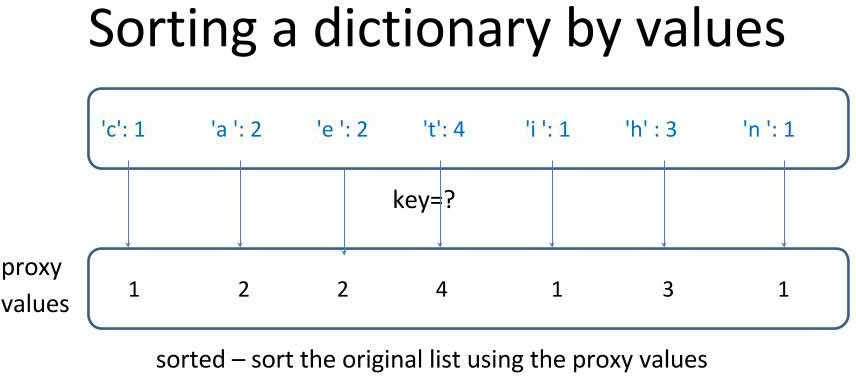
\includegraphics[scale=.37]{sortingbyvalue}\\
\end{figure}

We would like  the proxy values to be the letter counts

The question is how do we define our key argument function so that we end up with these proxy values?

We need the key argument function to return the value associated with the letter in the dictionary my{\_}count.  We can use the dictionary method \textit{get:}

my{\_}count.get(letter) returns the value associated with the argument letter in the dictionary. That's our letter count. To increment the count, we can use get() method and increase its value by 1 with each successive finding of a letter or word:

\begin{lstlisting}
with open(filename, 'r', encoding='utf-8') as my_file:
        # read line by line
        for line in my_file:
            line = line.lower()
            # read word by word
            for word in line.split():
                word = word.strip(string.punctuation + string.digits)
                if word:
                    word_dict[word] = word_dict.get(word, 0) + 1
\end{lstlisting}

We specify get as the key argument

\begin{lstlisting}
>>> my_count = {'c': 1, 'a': 2, 'e': 2, 't': 4, 'i': 1, 'h': 3, 'n': 1}

>>> sorted(my_count, key=my_count.get)

['c', 'n', 'i', 'e', 'a', 'h', 't'] 
\end{lstlisting}

Or to get the letter in decreasing order of frequency:

\begin{lstlisting}
>>> sorted(my_count, key=my_count.get, reverse=True)

['t', 'h', 'e', 'a', 'c', 'n', 'i']
\end{lstlisting}

To print these letters sorted by decreasing frequency, we can iterate over the list generated by sorted as follows:

\begin{lstlisting}
>>> sorted_letters = sorted(my_count, key=my_count.get, reverse=True)

>>> for letter in sorted_letters:

        print (letter + ':', my_count[letter])

t: 4

h: 3

e: 2

a: 2

c: 1

n: 1

i: 1
\end{lstlisting}

We'll often see the above written more concisely as:

\begin{lstlisting}
for letter in sorted(my_count, key=my_count.get, reverse=True):

        print (letter + ':', my_count[letter])

t: 4

h: 3

e: 2

a: 2

c: 1

n: 1

i: 1
\end{lstlisting}

It is common to specify a lambda function expression as the value of the key argument. 

\begin{lstlisting}
>>> sorted(my_count, key=lambda letter: my_count[letter])

['c', 'i', 'n', 'a', 'e', 'h', 't']
\end{lstlisting}

The anonymous lambda function here takes a letter as its argument and returns the corresponding count. The above is equivalent to the following:

\begin{lstlisting}
def get_count(letter):

    return my_count[letter]

sorted(my_count, key=get_count)
\end{lstlisting}

\subsubsection{max and min with a key}

The max and min functions also take an optional key argument that works in a similar manner:

\begin{lstlisting}
>>> words = ['in', 'the', 'face', 'of', 'ambiguity', 'refuse', 'the', 'temptation', 'to', 'guess']

>>> sorted(words, key=len)

['in', 'of', 'to', 'the', 'the', 'face', 'guess', 'refuse', 'ambiguity', 'temptation']

>>> max(words, key=len)

'temptation'

>>> min (words, key=len)

'in'
\end{lstlisting}

Going back to our letter count example, we can get the letters with the highest and lowest frequencies:

\begin{lstlisting}
>>> my_count = {'c': 1, 'a': 2, 'e': 2, 't': 4, 'i': 1, 'h': 3, 'n': 1}

>>> max(my_count, key=my_count.get)

't'
\end{lstlisting}

Or using a lambda function expression:

\begin{lstlisting}
>>> min(my_count, key=lambda letter: my_count[letter])

'n'
\end{lstlisting}

\subsection{A Dictionary Example}

Our goal in this example is to investigate letter distributions in English.

We’ll start by picking some representative text:  the lyrics to the Beatles song \textit{Yesterday}.

Since we have not yet seen how to read from a text file in Python, let's use a string variable for our song lyrics:

\begin{lstlisting}
song = '''
        Yesterday, all my troubles seemed so far away
        Now it looks as though they're here to stay
        Oh, I believe in yesterday
        Suddenly, I'm not half the man I used to be
        There's a shadow hanging over me.
        Oh, yesterday came suddenly
        Why she had to go I don't know she wouldn't say
        I said something wrong, now I long for yesterday
        Yesterday, love was such an easy game to play
        Now I need a place to hide away
        Oh, I believe in yesterday
        Why she had to go I don't know she wouldn't say
        I said something wrong, now I long for yesterday
        Yesterday, love was such an easy game to play
        Now I need a place to hide away
        Oh, I believe in yesterday
        '''
\end{lstlisting}
        
So we need to count the letters in the song.  Let's define a function \textit{count{\_}letters} to do that.

First note that the song has upper and lower case letters.  We want to treat them as the same letter.  We won't differentiate between Y and y.  We'll use the string method lower to get a lower case version of the text before performing the count.  

There is also a number of punctuation characters such as periods, commas and apostrophes that we don't care about counting.  We don't want to count white space either.  So we'll import the string module to get access to the string constant \textit{string.ascii{\_}lowercase}.  We'll only count the letters in there.

We have already seen how to use the count method on strings to count the number of occurrences of a given character.  We'll use count in our function.

We'll create a dictionary entry for each letter and assign a value to it.

Here's our function definition: 

\begin{lstlisting}
import string
def count_letters(text):
    """
    count the letters found in the string text

    Parameters: text, a string
    Returns: a dictionary with items of the form letter: count
    '''
    letter_count = {}             # initialize the dictionary
    lower_text = text.lower()     # convert the text to lower case
    # no need to count punctuation characters - go over the lower case letters
    for letter in string.ascii_lowercase:
        if letter in lower_text: # do not include letters with 0 count
            letter_count[letter] = lower_text.count(letter) # save the count
    return letter_count           # return the dictionary
\end{lstlisting}

We'll also write a function, \textit{report}, that takes the letter count dictionary as a parameter and prints the following:

\begin{itemize}
\item The total number of letters that appear at least once in the song.
\item The letters sorted alphabetically, with their corresponding count.
\item The letters sorted by count with the highest count letters first.
\end{itemize}

\begin{lstlisting}
def report(letter_count):
    """
    Print some statistics based on the given dictionary

    Parameter: 
    letter_count - a dictionary with items of the form letter: count
    Returns: None
    """
    print('The text contains', len(letter_count), 'letters')
    print("The letters sorted alphabetically:")
    for letter in sorted(letter_count):  # print letters in alphabetical order
        print(letter + ':', letter_count[letter])

    # build the list of letters sorted by decreasing frequency
    frequency_list = sorted(letter_count,
                            key=letter_count.get,
                            reverse=True)
    print("The letters sorted by frequency:")
    for letter in frequency_list:
        print(letter + ':', letter_count[letter])
\end{lstlisting}
        
Note that we used the two keyword parameters of the sorted function:  key and reverse.  

sorted(letter{\_}count, key=letter{\_}count.get, reverse=True) gives us a list of the dictionary keys (letters) sorted by the proxy value that is their corresponding count value.  We save that list in frequency{{\_}}list.

We then iterate over this list to print it.

Now in our main program, we'll include the following steps:
\begin{itemize}
\item Call count{\_}letters to build the song{\_}count dictionary.
\item Call report to print some statistics based on the song{\_}count dictionary.
\end{itemize}

\begin{lstlisting}
def main():
    song = '''
        Yesterday, all my troubles seemed so far away
        Now it looks as though they're here to stay
        Oh, I believe in yesterday
        Suddenly, I'm not half the man I used to be
        There's a shadow hanging over me.
        Oh, yesterday came suddenly
        Why she had to go I don't know she wouldn't say
        I said something wrong, now I long for yesterday
        Yesterday, love was such an easy game to play
        Now I need a place to hide away
        Oh, I believe in yesterday
        Why she had to go I don't know she wouldn't say
        I said something wrong, now I long for yesterday
        Yesterday, love was such an easy game to play
        Now I need a place to hide away
        Oh, I believe in yesterday
        '''
    song_count = count_letters(song)
    report(song_count)
\end{lstlisting}

\begin{lstlisting}
Putting it all together, here's our program:
# -------------------------------------------------------------------------------
# Name:        lettercount
# Purpose:     demonstrate the use of dictionaries
#
# Author:      Rula Khayrallah
#
# Created:     1/30/2015
#-------------------------------------------------------------------------------
"""
Count the letters in the Beatles song 'Yesterday'

Print all the letters found in the song alphabetically
followed by the number of times they appear in the song.
Print all the letters found in the song in descending order of frequency.
"""
import string

def count_letters(text):
    """
    count the letters found in the string text

    Parameters: text, a string
    Returns: a dictionary with items of the form letter: count
    """
    letter_count = {}          # initialize the dictionary
    lower_text = text.lower()  # convert the text to lower case
    # no need to count punctuation characters - go over the lower case letters
    for letter in string.ascii_lowercase:
        if letter in lower_text:
            letter_count[letter] = lower_text.count(letter)
    return letter_count        # return the dictionary


def report(letter_count):
    """
    Print some statistics based on the given dictionary

    Parameter: 
    letter_count - a dictionary with items of the form letter: count
    Returns: None
    """
    print('The text contains', len(letter_count), 'letters')
    print("The letters sorted alphabetically:")
    for letter in sorted(letter_count):  # print letters in alphabetical order
        print(letter + ':', letter_count[letter])
    # build the list of letters sorted by decreasing frequency
    frequency_list = sorted(letter_count,
                            key=letter_count.get,
                            reverse=True)
    print("The letters sorted by frequency:")
    for letter in frequency_list:
        print(letter + ':', letter_count[letter])

def main():
    song = '''
        Yesterday, all my troubles seemed so far away
        Now it looks as though they're here to stay
        Oh, I believe in yesterday
        Suddenly, I'm not half the man I used to be
        There's a shadow hanging over me.
        Oh, yesterday came suddenly
        Why she had to go I don't know she wouldn't say
        I said something wrong, now I long for yesterday
        Yesterday, love was such an easy game to play
        Now I need a place to hide away
        Oh, I believe in yesterday
        Why she had to go I don't know she wouldn't say
        I said something wrong, now I long for yesterday
        Yesterday, love was such an easy game to play
        Now I need a place to hide away
        Oh, I believe in yesterday
        '''
    song_count = count_letters(song)
    report(song_count)

if __name__ == '__main__':
    main()
\end{lstlisting}
And here's the corresponding output

\begin{lstlisting}
The text contains 22 letters
The letters sorted alphabetically:
a: 45
b: 5
c: 5
d: 28
e: 65
f: 4
g: 13
h: 27
i: 27
k: 3
l: 20
m: 10
n: 30
o: 43
p: 4
r: 19
s: 36
t: 31
u: 9
v: 6
w: 19
y: 34
The letters sorted by frequency:
e: 65
a: 45
o: 43
s: 36
y: 34
t: 31
n: 30
d: 28
h: 27
i: 27
l: 20
w: 19
r: 19
g: 13
m: 10
u: 9
v: 6
b: 5
c: 5
p: 4
f: 4
k: 3
\end{lstlisting}

\section{Files}
\subsection{Opening a File}

A file is a collection of data stored in one unit, identified by a file name. 

We may have:

\begin{itemize}
\item a text file: spider.txt
\item a program file: python.exe
\item an iTunes song: 02 Clocks.m4a
\item a picture: GrumpyCat.jpg
\end{itemize}

In Python, before we can read from or write to a file, we need to open it.  We use the built in function \textit{open} to do that.  The general syntax to open a file is as follows:

\begin{lstlisting}
some_file  = open(filename, mode, encoding)
\end{lstlisting}

The \textit{open} function returns a file handle.  We assign it to the variable \textit{some{\_}file}.  some{\_}file is just an arbitrary variable name.  We can use it  from there on to refer to the file. 

So, for example we can write:

\begin{lstlisting}
my_file = open('C:/Users/Rula/Documents/CS21A/spider.txt')
\end{lstlisting}

\subsubsection{Absolute and Relative Paths}
The file name above includes an absolute path: 'C:/Users/Rula/Documents/CS21A/spider.txt'.

Note that we used forward slashes. In Python, forward slashes always work, even on Windows.

We can also use a relative path as in:

\begin{lstlisting}
my_file = open('spider.txt')
\end{lstlisting}

The relative path will start from our working directory.  

To  figure out what our working directory is, we can use the \textit{os} module as follows:

\begin{lstlisting}
import os

print(os.getcwd())  
\end{lstlisting}

On windows, I get:

\begin{lstlisting}
C:\Users\Rula\Documents\CS21A
\end{lstlisting}

On a Mac OS:

\begin{lstlisting}
/Users/rulakhayrallah/PycharmProjects/CS21A
\end{lstlisting}

We’ll talk more about the os module later in the course.

It is best to use relative path names whenever possible to ensure the portability of our programs.  

\subsubsection{Mode}

\textit{mode} is an optional argument.   It defaults to 'rt' which means open for reading in text mode. So we can write:

\begin{lstlisting}
my_file = open('spider.txt', 'r')
\end{lstlisting}

The mode can be set to any of the following:
\begin{itemize}
\item 'r' open for reading (default).

\item 'w' open for writing, overwriting the existing file. 

\item 'x' create a new file for writing – generate an error if the file already exists.

\item 'a' open for writing, appending to the end of the  file if  it exists.

\item 'b'   binary mode.

\item 't'  text mode (default)

\item '+' open a file for reading and writing ('r+' or 'w+')
\end{itemize}

We can combine modes when it makes sense as in 'rt' (read in text mode) or 'w+b' (read/write in binary).

\subsubsection{Encoding}
\textit{Encoding} is also an optional keyword argument.  It is only applicable in text mode.  Encoding determines how the sequence of Unicode characters (text) is mapped onto bytes.  

\begin{lstlisting}
my_file = open('spider.txt', 'r', encoding='utf-8')
\end{lstlisting}

The encoding keyword argument is only available in Python 3.

The default encoding is platform dependent, but any encoding supported by Python can be passed.  

CP-1252 is a common encoding on computers running Microsoft Windows.

UTF-8 is used on Unix and Mac OS.

It is best to set the encoding to utf-8  when possible to make sure that our programs are platform independent.

\subsection{Closing a File}

When we're done with a file, we should close it.  To do that, we use the close method as follows:

\begin{lstlisting}
my_file = open('spider.txt', 'r', encoding='utf-8')

my_file.close()
\end{lstlisting}

We can test if the file is closed by checking the value of \textit{closed},   a boolean attribute defined on the file object.    closed indicates the state of the file.  It is True if the file is closed and False otherwise.

\begin{lstlisting}
>>> my_file = open('spider.txt', 'r', encoding='utf-8')

>>> my_file.closed

False

>>> my_file.close()

>>> my_file.closed

True
\end{lstlisting}

So typically, we open the file, do something with it then close it.

\begin{lstlisting}
some_file.open(filename,…)

Do something with the file

some_file.close()
\end{lstlisting}

If something happens while we are working with the file, that file could stay open for much longer than necessary.

In the next section, we'll introduce a way to get around this problem.

\subsection{A Better Way - The "With" Statement}

The \textit{with} statement offers us a safer way to open and close files.

\begin{lstlisting}
with open('spider.txt', 'r', encoding='utf-8') as my_file:
    do something with the file my_file
\end{lstlisting}

Let's take note of the following:

Here again, my{\_}file is an arbitrary variable name. We can use it  from there on to refer to the file. (It is the file handle).  It is as if we had:
 
\begin{lstlisting}
my_file = open('spider.txt', 'r', encoding='utf-8')
\end{lstlisting}
 
The \textit{with} statement starts a code block, like an if statement or a for loop.  Note the colon at the end of the with statement.  The code block after the with statement is indented.

We get to do whatever we need to do with my{\_}file inside the indented code block.
When the \textit{with} block ends, Python calls my{\_}file.close() automatically.

\subsubsection{Advantage}
No matter how or when we exit the with block, Python will close that file… even if our code crashes. 

In this course, we'll always use the \textit{with} statement when working with files.

\subsection{Reading the Whole File}

We can read the whole file at once.  We use the \textit{read} method to do that:

\begin{lstlisting}
with open('spider.txt', 'r', encoding='utf-8') as my_file:
         text = my_file.read()
print (text)

The Itsy Bitsy Spider went up the water spout.
Down came the rain, and washed the spider out.
Out came the sun, and dried up all the rain,
And the Itsy Bitsy Spider went up the spout again.
\end{lstlisting}

Here we are reading the whole file into a variable, \textit{text} – \textit{text} is a string.

Note that the print statement is outside the 'with' indented block.  At this point, the file is closed.  The content of the file has been saved in the variable \textit{text} and we can access it in our program even though the file has been closed.

We can add some more statements to manipulate or extract some specific data from the file we just read:  we'll use the \textit{lower} string method to get a copy of the text we just read in lower case and then print it.  We'll also use the \textit{count} string method to get the number of times 'spider' or 'spout'  appeared in the text we just read.

\begin{lstlisting}
with open('spider.txt', 'r', encoding='utf-8') as my_file:
         text = my_file.read()
print (text)
lower_text = text.lower()
print (lower_text)   # print a lower case version of the song
print ('spider ->', lower_text.count('spider'))  # print some statistics
print ('spout ->', lower_text.count('spout'))
 
The Itsy Bitsy Spider went up the water spout.
Down came the rain, and washed the spider out.
Out came the sun, and dried up all the rain,
And the Itsy Bitsy Spider went up the spout again.
the itsy bitsy spider went up the water spout.
down came the rain, and washed the spider out.
out came the sun, and dried up all the rain,
and the itsy bitsy spider went up the spout again.
spider -> 3
spout -> 2
\end{lstlisting}

Note that reading the whole file at once with the read method is only feasible if the file is small enough.  

\subsection{Reading One Line at a Time}

We can read the file one line at a time as follows:

\begin{lstlisting}
with open('spider.txt', 'r', encoding='utf-8') as my_file:
    for line in my_file:
        print(line)
\end{lstlisting}

Here again, \textit{line} is an arbitrary variable name.

We can think of a text file as a sequence of items where each item is a line.  We can iterate over the sequence with a for... in loop.  When we do, we get one line at a time.  So it is helpful (but not necessary) to call our iteration variable \textit{line} so we know what kind of entity we are dealing with.

\begin{lstlisting}
with open('spider.txt', 'r', encoding='utf-8') as my_file:
    for line in my_file:
        print(line)
 
The Itsy Bitsy Spider went up the water spout.
 
Down came the rain, and washed the spider out.
 
Out came the sun, and dried up all the rain,
 
And the Itsy Bitsy Spider went up the spout again.
\end{lstlisting}

We end up with extra lines in the output because each line read from the file (except the last one) has a new line character included in it.  Then \textit{print} appends a new line each time it is called.

To fix that, we can specify the \textit{end} parameter for print. This way it will NOT default to new line.

\begin{lstlisting}
with open('spider.txt', 'r', encoding='utf-8') as my_file:
    for line in my_file:
        print(line, end='')


The Itsy Bitsy Spider went up the water spout.
Down came the rain, and washed the spider out.
Out came the sun, and dried up all the rain,
And the Itsy Bitsy Spider went up the spout again.
\end{lstlisting}

\subsection{One Word at a Time?}

Often, our goal is to get to the individual words in the file, to analyze them or extract some information from them.  We can do that by using the string method \textit{split} on each line.  The \textit{split} method splits a string into a list of strings based on some delimiter. The default delimiter is white space, but it could be anything we specify.

\begin{lstlisting}
with open('spider.txt', 'r', encoding='utf-8') as my_file:
    for line in my_file:
        for word in line.split():
            print(word)
 
The
Itsy
Bitsy
Spider
went
up
the
water
spout.
Down
came
the
rain,
and
washed
the
spider
out.
Out
…
\end{lstlisting}

Note that since \textit{split} determined the boundaries of words using white space,  not punctuation, 'spout.' and 'rain,' were identified as words.

To fix that, we can use the string method \textit{strip}  and the constant string.punctuation as follows:

\begin{lstlisting}
import string
with open('spider.txt', 'r', encoding='utf-8') as my_file:
    for line in my_file:
        for word in line.split():
            word = word.strip(string.punctuation)  # get rid of punctuation
            print(word)
 
The
Itsy
Bitsy
Spider
went
up
the
water
spout
Down
came
the
rain
and
washed
the
spider
out
Out
...
\end{lstlisting}

Note that the variable names \textit{my{\_}file}, \textit{line} and \textit{word} are completely arbitrary.  We could have used x, y and z but then we would have quickly lost track of what we're dealing with.  

It is best to use representative variable names so we know what entity we're working with.

\subsection{Writing to a File}

Now that we know how to read a file, let's see how to write to it. 

We can append text to the end of the file.  To do that we specify 'a' for the mode. 
We can also overwrite an existing file by using the 'w' mode.

\subsubsection{Appending to a file - the 'a' mode}

\begin{lstlisting}
with open('spider.txt', 'a', encoding='utf-8') as my_file:

    my_file.write('And again and again.')
\end{lstlisting}

The write method writes a string to the file.  Note that the argument specified to \textit{write} has to be a string.  If we are writing a number, we need to convert it to a string first.

Our file spider.txt now contains the following:

The Itsy Bitsy Spider went up the water spout.

Down came the rain, and washed the spider out.

Out came the sun, and dried up all the rain,

And the Itsy Bitsy Spider went up the spout again.And again and again.

The write() method does not start a new line.  If we need a new line, we add the new line character to the string we are writing:

\begin{lstlisting}
with open('spider.txt', 'a', encoding='utf-8') as my_file:

    my_file.write('\nAnd again and again.')
\end{lstlisting}

spider.txt now contains the following:

The Itsy Bitsy Spider went up the water spout.

Down came the rain, and washed the spider out.

Out came the sun, and dried up all the rain,

And the Itsy Bitsy Spider went up the spout again.And again and again.

And again and again.

\subsubsection{Overwriting a file - the 'w' mode}

We can also overwrite an existing file by using the 'w' mode:

\begin{lstlisting}
with open('spider.txt', 'w', encoding='utf-8') as my_file:

    my_file.write('Bye Bye Spider')
\end{lstlisting}

spider.txt now contains the following:

Bye Bye Spider

Note that we don’t have to actually write something in 'w'  mode to overwrite the file.

Just opening it in 'w'  mode will overwrite it.

\begin{lstlisting}
with open('spider.txt', 'w', encoding='utf-8') as my_file:

    pass
\end{lstlisting}

spider.txt  is now empty.

The \textit{pass} statement does nothing.  It is simply used as a placeholder because the syntax of the \textit{with} statement requires an indented block. 

\subsection{Creating a New File}

Both the append mode 'a' and the write mode 'w' will create the file if it does not already exist:

\begin{lstlisting}
with open('newspider.txt', 'w', encoding='utf-8') as my_file:

    my_file.write('This is a brand new spider')

with open('newestspider.txt', 'a', encoding='utf-8') as my_file:

    my_file.write('This is a brand new spider')
\end{lstlisting}

The files newspider.txt and newestspider.txt are created in the working directory and  contain the following:

This is a brand new spider

We can also use the 'x' mode to create a file.

\begin{lstlisting}
with open('anotherspider.txt', 'x', encoding='utf-8') as my_file:

    my_file.write('This is a yet another spider')
\end{lstlisting}

The file anotherspider.txt is created in the working directory and  contains the following:

This is a yet another spider

With the 'x' mode, an error is generated  if the file already exists.

\subsection{A Spell Checker Example}

Our task today is to build a rudimentary spell-checker.

We’ll 'learn' the words by reading a very large text file and identifying the words in it.  The words in that reference file are assumed to be spelled correctly. Then we'll read an input file and identify the words in it as well.  Any word in the input file that is not found in the reference file is flagged as a potential misspelled word.

It looks like we have three major subtasks here:

\begin{itemize}
\item 'Learn' the words by reading a very large text file and identifying the words in it.  
\item Read an input file and identify the words in it.
\item Flag any word in the input file that is not found in the reference file as a potential misspelled word.
\end{itemize}

What data structure do we use to keep track of all the words we encounter?  List, tuple, set, dictionary?

A set seems like a good choice.  We only need to store a word once, even if it appears multiple times in a given file. We don’t need to keep the words in any order:  we’ll just need to check if a word exists or not.  Sets are an efficient choice for testing membership.

The first and second subtasks are very similar. We'll be reading a file and identifying the words in it.  In the first case it is the reference file and in the second it is the input file.  We'll implement one generic function that does that.  We learned in module 10.6 how to do that:

\begin{lstlisting}
import string
def get_words(filename):
    """
    Get the words from a file

    Parameter: file name
    Return: a set containing all the words in that file
    """
    words_set = set()
    with open(filename, 'r', encoding='utf-8') as file:
        for line in file:
            line = line.lower() #  convert the line to lower case
            for word in line.split():  #  then split it into words
                # take out leading and trailing special characters
                word = word.strip(string.punctuation + string.digits)
                if word:   # if word is not an empty string
                    words_set.add(word)  # add the word to our set
    return words_set
\end{lstlisting}

Here are a few observations about the code above:

We always use the with construct to open and close files.  
filename is the name of the file on our computer and file is the variable that we'll use to refer to that file inside my program. 
Since the file is very large, we read it line by line. When we iterate over a file with a for loop, we get one line in each iteration.  
We use the string method  lower to convert the line to lower case.
Remember that line.split() returns a list of the words in the string, line, using white space as the delimiter string.
We iterate over this list with a for loop, expecting one word in each iteration.
We take out leading and trailing punctuation characters.  We also take out leading and trailing numbers.  This may result in an empty string if the initial word only contained punctuation characters or numbers so we make sure that the resulting word is not the empty string (if word:) before adding it to our set. 
Our third subtask can be achieved by taking the difference of two sets:  the set of words in the input file - the set of words in the reference file - these are the misspelled words.

\begin{lstlisting}
def flag_misspellings(words, ref):
    """
    Identify misspellings in a set of words based on a reference set.

    Parameters: 
    words:  set of input words
    ref: set of reference words - these are correctly spelled words

    Return: None
    """
    misspellings = words - ref  # get the misspelled words
    if misspellings:   # if the set is not empty
        print ('The following words may have been misspelled:')
        for word in misspellings:
            print (word)
\end{lstlisting}

Putting it all together, we can then write our program as follows:

\begin{lstlisting}
# -----------------------------------------------------------------------------
# Name:        spellcheck
# Purpose:     Demonstrate files and the use of sets
#
# Author:      Rula Khayrallah
#
# Created:     9/30/2016
# -----------------------------------------------------------------------------
"""
A rudimentary spell checker

Prompt the user to enter a reference file name and an input file name.
This can be any text file in any language.
The program detects spelling errors in the input file name
and prints them out.
The program determines that a word is an error if it has not been seen
it in the reference.
"""
import string
def get_words(filename):
    """
    Get the words from a file

    Parameter: file name
    Return: a set containing all the words in that file
    """
    words_set = set()
    with open(filename, 'r', encoding='utf-8') as file:
        for line in file:
            line = line.lower() #  convert the line to lower case
            for word in line.split():  #  then split it into words
                # take out leading and trailing special characters
                word = word.strip(string.punctuation + string.digits)
                if word:   # if word is not an empty string
                  words_set.add(word)  # add the word to our set
    return words_set


def flag_misspellings(words, ref):
    """
    Identify misspellings in a set of words based on a reference set.

    Parameters: 
    words:  set of input words
    ref: set of reference words - these are correctly spelled words

    Return: None
    """
    misspellings = words - ref  # get the misspelled words
    if misspellings:   # if the set is not empty
        print ('The following words may have been misspelled:')
        for word in misspellings:
            print (word)


def main():
    ref_name = input('Please enter the reference file name: ')
    reference = get_words(ref_name)   # get the reference words
    input_name = input('Please enter the input file name: ')
    input_words = get_words(input_name)  # get the input words
    flag_misspellings(input_words, reference)


if __name__ == '__main__':
    main()
\end{lstlisting}

We can test our spell checker at this point:

Using 'Pride and Prejudice' by Jane Austen (1813) as our reference and a recent technology news article, we get the following:

The following words may have been misspelled:

developers

storage

push

notifications

apps

google

mobile

backend

starter

bitcoin

ios

code

queries

blog

We can even test with text in different languages:

Using 'Les Miserables' by Victor Hugo as our French language reference and a French children song – spelled correctly, we get the following:

The following words may have been misspelled:

plumerai

\section{Object-Oriented Programming}

\subsection{When and Why?}

Object oriented programming started in the Artificial Intelligence community in the 1960s.  However the term 'object oriented programming' was not introduced until the 1970s.

In the late 1980s and 1990s it became the main programming paradigm used in the creation of new software. It was well suited to handle the rapidly increasing size and complexity of software.

Object-oriented features have been added to many previously existing languages.

Python was designed to support object-oriented programming while still compatible with functional methodology. 

\subsection{What's an Object?}

So far we have been talking about functions and data:  functions perform some operations and return data and data is operated upon. 

An object, on the other hand is an abstraction that combines information and behavior.   We can think of it as a building block with some desired functionality.  The functionality is encapsulated in the object:  we know the 'what' not the 'how'.

Let's take a look at some object examples next.

An object example - a car:

A car has some attributes: make, model, mileage, fuel efficiency, etc…
But it also has a certain behavior.
When we drive the car, we use up some gas.
When we drive the car, the car mileage increases.
At some point, we may run out of gas.
We may fill up the tank with gas, and so on…
Let’s try to organize these attributes and behavior:

Attributes:

make
model
mileage
gas in tank
fuel efficiency
Behavior:

drive (6 miles) 
add gas(7.6 gallons)
Another object example: a bank account

Attributes:

owner : 'Alex' 
balance: {\$}20
Behavior:

deposit ({\$}100)
withdraw({\$}20)
One last object example: a person

Attributes:

name
birthday
profile picture
friends
Behavior:

 add a friend(person)
 unfriend(person)
OOP Terminology:

The attributes correspond to the fields, properties or instance variables.

The behavior corresponds to the methods.

In OOP, we say that methods are invoked on a particular object. 

In Python everything is an object. 

Integers, strings, lists, dictionaries are objects.  Data types, functions and modules are also objects.

And of course, we'll create our own objects.

\subsection{Classes}

A class is a group of objects with common behavior.  The class definition contains a template for the objects.

Defining a class in Python is simple. We define the class and start coding. 

\begin{lstlisting}
class Car(object):
   
    """
    Represent a car in  my virtual world.
    """
\end{lstlisting}
    
A Python class starts with the reserved word class, followed by the class name.

The header indicates that the new class is a Car, which is a kind of object. object is a built-in type.

Class names are usually capitalized and use CapWords.

Just like function definitions and compound statements, the class definition header ends with a colon.

Everything in a class  definition is indented. The first line not indented is outside the class.

We can define methods inside a class definition, we'll see how to do that in the upcoming sections.

The docstring  explains what the class is for. The docstrings conventions document (PEP 257 - available from the left navigation tab) recommends inserting  a blank line before and after all docstrings that document a class.

Later on, we'll come back to this class docstring and add more details to describe the Car object.

The class is like a factory for creating objects. To create a Car object, we call Car as if it were a function.

\begin{lstlisting}
my_car = Car(...)
\end{lstlisting}

Creating a new object is called instantiation, and the object is an instance of the class.

The above statement creates a new instance of the class Car and assigns this object to the local variable my{\_}car.

There is no explicit new operator like in other languages.

Some classes inherit from other classes.  Car just inherits from the object built-in class.   We’ll cover inheritance a little later.

There is nothing that a Python class absolutely must have, other than a name. 

The {\_}{\_}init{\_}{\_} method:

The method that initializes objects has a special name, {\_}{\_}init{\_}{\_}.

Think of it as the constructor for the class – even though the object has already been created.

It is not required, but if it is there it is called immediately after an instance of the class is created.

By convention, the {\_}{\_}init{\_}{\_} method is the first method defined for the class.

\begin{lstlisting}
class Car(object):
   
    """
    Represent a car in  my virtual world.
    """
    def __init__(self,  make,  model, fuel_efficiency, mileage=0, gas=0):
\end{lstlisting}

The first parameter of a method is a reference to the current instance of the class. 

By convention, this parameter is named self. (Other languages use 'this' instead.)

self is not a reserved word in Python.  It’s a naming convention.

We need to specify self explicitly when defining the method.  However we do  not specify it when calling the method.  Python will add it for us automatically.

Where do the rest of {\_}{\_}init{\_}{\_}’s arguments come from?

Remember that to create a  Car object, we call Car as if it were a function.  This is where we pass the arguments that will be used by {\_}{\_}init{\_}{\_}.

\begin{lstlisting}
my_car = Car('Honda', 'Civic', 28)
\end{lstlisting}

Now is a good time to go back to the Car class docstring and update it to reflect the arguments that {\_}{\_}init{\_}{\_} needs.

\begin{lstlisting}
class Car(object):
 
    """
    Represent a car in  my virtual world.
 
    Arguments:
    make (string): car make.
    model (string): car model.
    fuel_efficiency (float): in miles per gallon.
    mileage (float, optional): current mileage on car in miles, defaults to 0.
    gas (float, optional): current gas in the tank in gallons, defaults to 0.   
\end{lstlisting}

\subsection{Instances}

To instantiate a class, we simply call the class as if it were a function, passing the arguments that the {\_}{\_}init{\_}{\_} method requires.

The return value will be the newly created object.  We call that the new instance.

\begin{lstlisting}
my_car = Car('Honda','Civic', 28, 12000, 3.5)
\end{lstlisting}

When we call the print function on an instance, Python usually tells us what class it belongs to.

\begin{lstlisting}
print(my_car)

<__main__.Car object at 0x02D34450>
\end{lstlisting}

\subsection{Instance Variables}

What does an object need to remember?

Car:  gas, mileage, make, model, fuel efficiency
Account: holder, balance
Instance variables are the attributes that are specific to the instance.  Each object (or instance) has a separate copy of the instance variable.

Let’s go back and fill in the code for our {\_}{\_}init{\_}{\_} method in the Car class:

\begin{lstlisting}
class Car(object):

    """
    Represent a car in  my virtual world.

    Arguments:
    make (string): car make.
    model (string): car model.
    fuel_efficiency (float): in miles per gallon.
    mileage (float, optional): current mileage on car in miles, defaults to 0.
    gas (float, optional): current gas in the tank in gallons, defaults to 0.
    """

    def __init__(self,  make,  model, fuel_efficiency, mileage=0, gas=0):
        self.make = make
        self.model = model
        self.fuel_efficiency = fuel_efficiency
        self.mileage = mileage
        self.gas_in_tank = gas
\end{lstlisting}
        
In Python, we use the dot notation to designate an attribute (or instance variable) of an object.
self.make, self.model, self.fuel{\_}efficiency, self.mileage and self.gas{\_}in{\_}tank are all attributes of the object. They are also called "instance variables.

They are global to the instance. That means that we can access them from other methods.

self.make, self.model, self.fuel{\_}efficiency, self.mileage and self.gas{\_}in{\_}tank are separate from the {\_}{\_}init{\_}{\_} parameters make, model, fuel{\_}efficiency, mileage and gas.  The names don’t have to be the same.

We can go back and expand our class docstring to document these instance variables.

\begin{lstlisting}
class Car(object):

    """
    Represent a car in  my virtual world.

    Arguments:
    make (string): car make.
    model (string): car model.
    fuel_efficiency (float): in miles per gallon.
    mileage (float, optional): current mileage on car in miles, defaults to 0.
    gas (float, optional): current gas in the tank in gallons, defaults to 0.

    Attributes:
    make (string): car make.
    model (string): car model.
    fuel_efficiency (float): in miles per gallon.
    mileage (float): current mileage on the car in miles.
    gas_in_tank (float): current gas in the tank in gallons.
    """

    def __init__(self,  make,  model, fuel_efficiency, mileage=0, gas=0):
        self.make = make
        self.model = model
        self.fuel_efficiency = fuel_efficiency
        self.mileage = mileage
        self.gas_in_tank = gas
\end{lstlisting}

Instance variables are specific to one instance of a class. For example, if we create two Car instances with different make and model, they will each remember their own make and model.

A little demo:

\begin{lstlisting}
>>> from car import Car
\end{lstlisting}

My class definition for the class Car is saved in a module named car.py.

We have seen how to import the whole module before: import car.

However that would mean every time I want to call Car from the interpreter or from outside the module,  I have to prefix with the module name:

\begin{lstlisting}
my_car = car.Car('Honda', 'Civic', 28)
\end{lstlisting}

When I use from car import Car, I can just use Car without prefixing it with the module name:

\begin{lstlisting}
>>> from car import Car

>>> my_car = Car('Honda', 'Civic', 28)
\end{lstlisting}

Here I have just created a new instance of the Car class.  I also have assigned that new instance to the variable my{\_}car.

\begin{lstlisting}
>>> your_car = Car('Porsche', '911', 23)
\end{lstlisting}

...and another instance of the Car class assigned this time to the variable your{\_}car.

\begin{lstlisting}
>>> print(my_car.make)

Honda

>>> print(your_car.make)

Porsche
\end{lstlisting}

These are two different instance variables, associated with two different objects. 

my{\_}car and your{\_}car are 2 different instances, 2 different objects

Each instance will remember its own make, its own model and its own fuel{\_}efficiency.

\begin{lstlisting}
>>> print(my_car.model)

Civic

>>> print(your_car.model)

911

>>> print(my_car.fuel_efficiency)

28

>>> print(your_car.fuel_efficiency)

23
\end{lstlisting}

\subsection{Identity}

Each new car instance has its own attributes (make, model, etc.) and the value of these attributes is independent of other objects of the same class.

To enforce this separation, every object has a unique identity.

Object identity is compared using the is and is not operators.

\begin{lstlisting}
>>> my_car = Car('Honda', 'Civic', 28)

>>> his_car = Car('Honda', 'Civic', 28)
\end{lstlisting}

my{\_}car and your{\_}car are two different objects.

\begin{lstlisting}
>>> my_car is his_car

False
\end{lstlisting}

Even though they are constructed from identical calls, the objects my{\_}car and his{\_}car are not the same. Two separate objects have been created here.

Note that in English, I would say that he and I have the same car:  same make, same model, maybe even same color.   But that does not mean the same physical car!  We each have our own car, we do not share a car.

\subsubsection{Identity and Assignment}

Now consider the following:

\begin{lstlisting}
>>> his_car = Car('Honda', 'Civic', 28)

>>> her_car = his_car

>>> her_car is his_car

True
\end{lstlisting}

As we’ve seen before with lists, an assignment does not create a new object.  his{\_}car and her{\_}car are pointing to the same object in memory.

New objects are only created when a class is instantiated with Car(...).

his{\_}car and her{\_}car point to the same object

\begin{lstlisting}
>>> print(his_car.fuel_efficiency)

28

>>> print(her_car.fuel_efficiency)

28

>>> his_car.fuel_efficiency = 22

>>> print(her_car.fuel_efficiency)

22 
\end{lstlisting}

Because his{\_}car and her{\_}car are pointing to the same object, changing his{\_}car.fuel{\_}efficiency changes her{\_}car.fuel{\_}efficiency.

\subsection{Methods}

Methods describe what we do with the objects.

The bank account:

deposit
withdraw

The car:

add gas
drive

Methods are basically functions that operate on the object or perform object-specific computations.

We say that methods are invoked on a particular object.

Methods are defined inside a class definition in order to make the relationship between the class and the method explicit.

\subsubsection{Defining a method}

Let's define the first method for our Car class.  Remember that we are trying to capture the behavior of the car and encapsulate it in the object.

Behavior:  Adding  gas to the car

We define a method with the def keyword just as we would define a function.

\begin{lstlisting}
    def add_gas(self, amount):

        """
        Add gas to the car.
        Parameter:
        amount (float): the amount of gas to be added in gallons.
        Return:
        the updated car object (Car).
        """
        self.gas_in_tank += amount
        return self
\end{lstlisting}

A method has a docstring just like a function.  That docstring is available when we get help on the class Car:

\begin{lstlisting}
>>> from car import Car
>>> help(Car)

Help on class Car in module car:
class Car(builtins.object)
 |  Represent a car in  my virtual world.
 | 
 |  Arguments:
 | … 
 |  Attributes:
 | … 
 |  Methods defined here:
 | 
 |  __init__(self, make, model, fuel_efficiency, mileage=0, gas=0)
 |  
 |  add_gas(self, amount)
 |      Add gas to the car.
 |      Parameter:
 |      amount (float): the amount of gas to be added in gallons.
 |      Return:
 |      the updated car object (Car).
 |  
\end{lstlisting}

We can also get help on the method directly, we just prefix it with the class name.

\begin{lstlisting}
>>> help(Car.add_gas)

Help on function add_gas in module car:
 
add_gas(self, amount)
    Add gas to the car.
    Parameter:
    amount (float): the amount of gas to be added in gallons.
    Return:
    the updated car object (Car).
\end{lstlisting}

Method definitions include the special first parameter \textit{self}.  self refers to the object on which the method is invoked. In our examples self will point to my{\_}car or your{\_}car or his{\_}car.  All methods have access to the object via the self parameter, and so they can all access and manipulate the object's state.

The add{\_}gas method takes an amount parameter:  it is listed after self in the function definition.

To access an attribute of a particular object inside the method, we use self.attribute{\_}name.  gas{\_}in{\_}tank is an attribute of our car objects (an instance variable).  To access the gas{\_}in{\_}tank attribute of a given instance, we use self.gas{\_}in{\_}tank.

Note that the add{\_}gas method returns the updated car object, self. When we write methods that return updated objects, we can chain method invocations so that the object is operated on by several methods sequentially.  We'll see how to take advantage of that in the next section.

And this is how everything fits together:

The method definition is inside the class definition and the class definition is inside the module car.py

\subsubsection{Invoking a method}
The syntax for invoking a method is different from the syntax for calling a function. 

The method is invoked on an object and the self parameter does not have to be specified.

From the interpreter, we can write:

\begin{lstlisting}
>>> from car import Car

>>> my_car = Car('Honda', 'Civic', 28)

>>> my_car.add_gas(12.5)

<car.Car object at 0x0000000003626A90>

>>> print(my_car.gas_in_tank)

12.5
\end{lstlisting}

\subsection{More Methods for Our Car}

Now we can go ahead and define more methods for our class.  Remember that we are trying to capture the behavior of the car and encapsulate it in the object.

\subsubsection{Behavior: Driving the car}

We drive the car a given distance.  We'll define the requirements on our drive method interface as follows:

 Parameter:

 distance (float):  the distance to be driven in miles.

 Return:

 the updated car object (Car).

The method definition will then start with:

def drive(self, distance):

Here again, the first parameter to the drive method is self.  The distance parameter is listed after self.
Before writing the method definition, let’s work through an example.

Suppose we have 3 gallons of gas in the tank in the car object our{\_}car.

Our fuel efficiency is 25 miles per gallon.

If we invoke drive on our car:

our{\_}car.drive(25) – > we expect success

The  mileage on the car needs to be updated:

mileage = mileage + 25

mileage = mileage + distance

The gas in the tank needs to be updated. 

We use up one gallon to drive 25 miles, so:

gas in tank = gas in tank – 1

gas in tank = gas in tank – (distance / fuel efficiency )

Now suppose that we want to drive another 100 miles.

At this point we have 2 gallons of gas in the tank.

Our fuel efficiency is still 25 miles per gallon.

If we invoke drive on our car:

our{\_}car.drive(100) – > we expect to run out of gas 

That’s because with 2 gallons in the tank, the maximum distance we can drive is 25 * 2 = 50 miles

maximum distance = fuel efficiency * gas in tank

So we expect the car to go for 50 miles and then stop because it’s out of gas.

The  mileage on the car needs to be updated:

mileage = mileage + maximum distance

The gas in the tank needs to be updated: the tank is empty at this point. 

gas in tank = 0

\subsubsection{Method Definition:  drive}

Now we can write our method definition as follows. 

\begin{lstlisting}
    def drive(self, distance):
        """
        Drive a car a given distance, if possible.
        If there is not enough gas, drive as much as possible.
        Parameter:
        distance (float):  the distance to be driven in miles.
        Return:
        the updated car object (Car)
        """
        max_distance = self.fuel_efficiency * self.gas_in_tank
        if distance <= max_distance:  # we can drive the distance
            self.mileage += distance
            self.gas_in_tank = self.gas_in_tank - \
                               distance / self.fuel_efficiency
        else:   # not enough gas
            self.mileage += max_distance  # drive as far as possible
            self.gas_in_tank = 0
        return self
\end{lstlisting} 

Note that we used the backslash  to indicate a multi-line statement.

\begin{lstlisting}
            self.gas_in_tank = self.gas_in_tank - \
                               distance / self.fuel_efficiency
\end{lstlisting} 

However the preferred way of wrapping long lines is by using Python's implied line continuation inside parentheses.  So instead of using the backslash, we can write: 

\begin{lstlisting}
             self.gas_in_tank = (self.gas_in_tank -
                                 distance / self.fuel_efficiency)
\end{lstlisting} 

And this is how everything fits together now in the module car.py:

\begin{lstlisting}
class Car(object):

    """
    Represent a car in  my virtual world.

    Arguments:
    make (string): car make.
    model (string): car model.
    fuel_efficiency (float): in miles per gallon.
    mileage (float, optional): current mileage on car in miles, defaults to 0.
    gas (float, optional): current gas in the tank in gallons, defaults to 0.

    Attributes:
    make (string): car make.
    model (string): car model.
    fuel_efficiency (float): in miles per gallon.
    mileage (float): current mileage on the car in miles.
    gas_in_tank (float): current gas in the tank in gallons.
    """

    def __init__(self,  make,  model, fuel_efficiency, mileage=0, gas=0):
        self.make = make
        self.model = model
        self.fuel_efficiency = fuel_efficiency
        self.mileage = mileage
        self.gas_in_tank = gas

    def add_gas(self, amount):
        """
        Add gas to the car.
        Parameter:
        amount (float): the amount of gas to be added in gallons.
        Return:
        the updated car object (Car).
        """
        self.gas_in_tank += amount
        return self

    def drive(self, distance):
        """
        Drive a car a given distance, if possible.
        If there is not enough gas, drive as much as possible.
        Parameter:
        distance (float):  the distance to be driven in miles.
        Return:
        the updated car object (Car)
        """
        max_distance = self.fuel_efficiency * self.gas_in_tank
        if distance <= max_distance:  # we can drive the distance
            self.mileage += distance
            self.gas_in_tank = (self.gas_in_tank - 
                                distance / self.fuel_efficiency)
        else:   # not enough gas
            self.mileage += max_distance  # drive as far as possible
            self.gas_in_tank = 0
        return self
\end{lstlisting}

\subsection{Class Variables}

Some attribute values are shared across all objects of a given class. Such attributes are associated with the class itself, rather than any individual instance of the class.

These attributes are also called class variables.

For instance, let us say that for all our cars in the Car class, we want to specify the distance unit (miles).  We want to remember this distance unit.  However it is the same for all the cars in our class.

Class variables are created by assignment statements in the class definition, outside of any method definition.

\begin{lstlisting}
class Car(object):

    """
    Represent a car in  my virtual world.

    Arguments:
    make (string): car make.
    model (string): car model.
    fuel_efficiency (float): in miles per gallon.
    mileage (float, optional): current mileage on car in miles, defaults to 0.
    gas (float, optional): current gas in the tank in gallons, defaults to 0.

    Attributes:
    make (string): car make.
    model (string): car model.
    fuel_efficiency (float): in miles per gallon.
    mileage (float): current mileage on the car in miles.
    gas_in_tank (float): current gas in the tank in gallons.
    """

    distance_unit = 'miles'

    def __init__(self,  make,  model, fuel_efficiency, mileage=0, gas=0):
        self.make = make
        self.model = model
        self.fuel_efficiency = fuel_efficiency
        self.mileage = mileage
        self.gas_in_tank = gas
\end{lstlisting}
 
distance{\_}unit is a class variable of the class Car.  It is available before creating any instances of the class.

Class variables are available through any instance of the class:

\begin{lstlisting}
>>> from car import Car

>>> my_car = Car('Honda','Civic', 25)

>>> print(my_car.distance_unit)

miles
\end{lstlisting}

They are also available through a direct reference to the class:

\begin{lstlisting}
>>>print(Car.distance_unit)

miles
\end{lstlisting}

Class variables can be used as class-level constants, but they are not really constants. We can also change them.  If we want to change them, we’ll have to do so through the reference to the class, not through an instance  reference.)

Let's see how that works:

\begin{lstlisting}
>>> from car import Car

>>> my_car = Car('Honda', 'Civic', 28)

>>> your_car = Car('Porsche', '911', 23)

>>> print(my_car.make)

Honda

>>> print(your_car.make)

Porsche

>>> print(Car.distance_unit)

miles

>>> print(my_car.distance_unit)

miles

>>> print(your_car.distance_unit)

miles
\end{lstlisting}

We have just created two instances of the Car class, my{\_}car and your{\_}car and we can access the class variable through either of them.

Now let's say we want to change the distance unit to km, and we first write:

\begin{lstlisting}
>>> my_car.distance_unit = 'km'

>>> print(my_car.distance_unit) 

km
\end{lstlisting}

Here we have created a new instance variable, distance{\_}unit.  We have not changed the class variable distance{\_}unit.

\begin{lstlisting}
>>> print(your_car.distance_unit)

miles

>>> print(Car.distance_unit)

miles
\end{lstlisting}

If we want to change the class variable, we’ll have to do so through the reference to the class:

\begin{lstlisting}
>>> Car.distance_unit = 'km'

>>> print(your_car.distance_unit)

km
\end{lstlisting}

\subsection{Private Instance Variables?}

Private instance variables that cannot be accessed except from inside an object don’t exist in Python.

We don’t need getter and setter methods to access instance variables.

Not only can we can access (read)  the car mileage, make, etc… from outside the class and from the interpreter prompt, we can also modify these instance variables from outside the class:

\begin{lstlisting}
>>> from car import Car

>>> my_car = Car('Honda','Civic', 25)

>>> print(my_car.mileage)

0

>>>my_car.mileage = 6000

>>> print(my_car.mileage)

6000
\end{lstlisting}

However, there is a convention that is followed by most Python code: a name prefixed with an underscore (for example  {\_}private) should be treated as a non-public part of the API (whether it is a function, a method or an instance variable).  It should be considered an implementation detail and subject to change without notice.

\subsection{Why OOP?}

Object Oriented Programming allows us to tame the size of complexity of software by dividing it into logical and semi independent entities.

It makes the maintenance of this software much easier to handle.

The interface becomes separate from the implementation. The interface has to keep track of the 'what' not the 'how'.  For objects, the methods a class provides should not depend on how the attributes are represented or manipulated. 

A method with a given interface may be implemented in several ways.

As a result, when we design the interface carefully, we can change the implementation when the need arises without changing the interface.

\section{Magic Methods}
\subsection{What are Magic Methods?}

Magic methods, also called special methods, are methods that we define to add magic to our classes. 

Their name is surrounded by double underscores ( like {\_}{\_}init{\_}{\_} or {\_}{\_}str{\_}{\_}).

Remember that in Python, anything that starts with {\_} is supposed to be private to the class and not part of the interface. The magic methods perform their magic behind the scenes but they are not supposed to be explicitly invoked from outside the class.

We have already seen the most basic magic method, {\_}{\_}init{\_}{\_}. 

{\_}{\_}init{\_}{\_} allows us to define  the initialization behavior of an object.

Even though it is NOT invoked explicitly, {\_}{\_}init{\_}{\_} gets magically invoked and passed whatever parameters are specified in the object instantiation.

\begin{lstlisting}
new_car = Car('Honda', 'Civic', 28)
\end{lstlisting}

In the next sections,  we'll examine some other useful magic methods in Python.

\subsection{The {\_}{\_}str{\_}{\_} Methods}

The {\_}{\_}str{\_}{\_} method is another magic method that we can define in our classes.

We define it to return a string representation of an object.  

When we print an object, Python invokes the {\_}{\_}str{\_}{\_} method on that object to figure out what to print.

It is very useful for debugging.

Let’s go back to our Car class definition.

We did not have a {\_}{\_}str{\_}{\_} method defined there.  What happens when we try to print a Car object?

\begin{lstlisting}
>>> from car import Car

>>> my_car = Car('Honda', 'Civic', 28)

>>> print(my_car)

<car.Car object at 0x02AB6CD0>
\end{lstlisting}

Now let’s add a {\_}{\_}str{\_}{\_} method definition to our Car class.

It goes right after the {\_}{\_}init{\_}{\_} method definition.

We can choose to return whatever we want to represent a car. 

Let’s just return the make and the model.

\begin{lstlisting}
    def __str__(self):

        return self.make + ' ' + self.model
\end{lstlisting}

Now what happens when we print a Car object?

\begin{lstlisting}
>>> from car import Car

>>> my_car = Car('Honda', 'Civic', 28)

>>> print(my_car)

Honda Civic
\end{lstlisting}

The {\_}{\_}str{\_}{\_} method is also invoked when we call the str function on an object.

\begin{lstlisting}
>>> from car import Car

>>> my_car = Car('Honda', 'Civic', 28)

>>> str(my_car)

'Honda Civic'
\end{lstlisting}

\subsection{Operator Overloading}

Changing the behavior of an operator so that it works with user-defined classes is called operator overloading. 

Python's magic methods provide a simple way to make objects behave like built-in types.  They allow us to specify the behavior of operators (+, -, ==, <, [], etc…) on any object.

We can  then use these operators on our own classes as if they were built-in types.  

For every operator in Python there is a corresponding special method.  

Let's go back to our car example and illustrate why it is convenient to have such methods.

\begin{lstlisting}
>>> my_car = Car('Honda', 'Civic', 28)

>>> his_car = Car('Honda' , 'Civic', 28)

>>> my_car is his_car 

False  
\end{lstlisting}

We have seen that my{\_}car and his{\_}car are two different objects.

However we still may want to capture the fact that these cars have the same make and model.

We could write a method in the Car class as follows:
\begin{lstlisting}
    def same_car(self, other):

        "returns True if both cars have the same make and model"

        result = (self.make == other.make) and (self.model == other.model)

        return result

>>> my_car = Car('Honda', 'Civic', 28)

>>> his_car = Car('Honda', 'Civic', 28)

>>> my_car.same_car(his_car)

True
\end{lstlisting}

However it would be nice if we did not have to create a new method name for such a method.  

It would be nice to use the == and have it mean 'same make and model' for our car objects.

And we can do that!

We just use the magic method {\_}{\_}eq{\_}{\_}.  It defines the  behavior for the equality operator, ==.

\begin{lstlisting}
    def __eq__(self, other):

        result = (self.make == other.make) and (self.model == other.model)

        return result
\end{lstlisting}

When we have a method that deals with two objects, we typically have two parameters: self and other.

And now we can simply use == on cars:

\begin{lstlisting}
>>> my_car = Car('Honda', 'Civic', 28)

>>> his_car = Car('Honda', 'Civic', 28)

>>> your_car = Car('Porsche', '911', 25)

>>> his_car == my_car

True

>>> your_car == my_car

False
\end{lstlisting}

When we write:  your{\_}car == my{\_}car

Python invokes:

\begin{lstlisting}
your_car. __eq__(my_car)
\end{lstlisting}

When we write:  his{\_}car == my{\_}car

Python invokes:
\begin{lstlisting}
his_car. __eq__(my_car)
\end{lstlisting}

And here's where the magic is!

\subsection{Rich Comparison Models}

At the beginning of this  course, we introduced the following comparison operators supported by Python:  ==, !=, <, >, <=, >=.

We have used these operators on the built in Python types integers and floats.  

Python allows us to define the behavior of all of these operators on our own objects by defining the special methods below:

\begin{lstlisting}
__eq__(self, other)  == equality operator  

__ne__(self, other)  != inequality operator 

__lt__(self, other)  < less-than operator

__gt__(self, other) > greater-than operator

__le__(self, other)  <= less-than-or-equal-to operator

__ge__(self, other)  >= greater-than-or-equal-to operator

When we write:	Python invokes:
x == y	x.__eq__(y)
x != y	x.__ne__(y)
x < y	x.__lt__(y)
x > y	x.__gt__(y)
x <= y	x.__le__(y)
x >= y	x.__ge__(y)
\end{lstlisting}

We have seen how to define  {\_}{\_}eq{\_}{\_} method for our Car class. 

However x == y being True does not imply that x != y is False. 

So when we define {\_}{\_}eq{\_}{\_} we should also define {\_}{\_}ne{\_}{\_} so that the operators will behave as expected. 

Let’s go back and define a {\_}{\_}ne{\_}{\_} method for our cars.

When we write x != y, Python will invoke:  x.{\_}{\_}ne{\_}{\_}(y)

{\_}{\_}ne{\_}{\_} compares two objects, so we need two parameters: self and other.

\begin{lstlisting}
    def __ne__(self, other):

        result = self.make != other.make or self.model != other.model

        return result
\end{lstlisting}

And we can test our new magic method as follows:

\begin{lstlisting}
>>> my_car = Car('Honda', 'Civic', 28)

>>> his_car = Car('Honda', 'Civic', 28)

>>> your_car = Car('Porsche', '911', 25)

>>> his_car == my_car

True

>>> his_car != my_car

False

>>> your_car == my_car

False

>>> your_car != my_car

True
\end{lstlisting}

Now let's define the {\_}{\_}lt{\_}{\_} (less than) method on our cars based on their mileage.

Remember that when we have a method that deals with two objects, we have 2 parameters: self and other.

\begin{lstlisting}
    def __lt__(self, other):

        return self.mileage < other.mileage
\end{lstlisting}

And we can test it as follows:

\begin{lstlisting}
>>> from car import Car

>>> my_car = Car('Honda', 'Civic', 28)

>>> my_car.add_gas(15)

<car.Car object at 0x00000000036B9E10>

>>> my_car.drive(35)

<car.Car object at 0x00000000036B9E10>

>>> his_car = Car('Porsche', '911', 25)

>>> his_car.add_gas(12)

<car.Car object at 0x00000000036B9E10>

>>> his_car.drive(200)

<car.Car object at 0x00000000036CF668>

>>> my_car < his_car

True

>>> his_car < my_car

False
\end{lstlisting}

When I write:  

\begin{lstlisting}
my_car <  his_car
\end{lstlisting}

Python invokes:

\begin{lstlisting}
my_car.__lt__(his_car)
\end{lstlisting}

When I write:  

\begin{lstlisting}
his_car <  my_car
\end{lstlisting}

Python invokes:
\begin{lstlisting}
his_car.__lt__(my_car)
\end{lstlisting}
 

\subsubsection{< and > Conversions?}
If we define a {\_}{\_}lt{\_}{\_} method but no {\_}{\_}gt{\_}{\_} method, Python will use the {\_}{\_}lt{\_}{\_} method with operands swapped.

\begin{lstlisting}
>>> his_car > my_car

True
\end{lstlisting}

Python converts it to: my{\_}car < his{\_}car and calls my{\_}car.{\_}{\_}lt{\_}{\_}(his{\_}car).

However, Python will not combine methods.

If we define a {\_}{\_}lt{\_}{\_} method and an {\_}{\_}eq{\_}{\_} method and try to test whether x <= y, Python will NOT call {\_}{\_}lt{\_}{\_} and {\_}{\_}eq{\_}{\_}. 

\begin{lstlisting}
>>> my_car <= his_car

Traceback (most recent call last):

  File "<input>", line 1, in <module>

TypeError: unorderable types: Car() <= Car()
\end{lstlisting}

The module functools provides a way to define all rich comparison methods if we only define {\_}{\_}eq{\_}{\_} and one other method.

\subsection{Arithmetic and Logical Operators Methods}

Python also allows us to define the behavior of arithmetic and logical operators on our own objects by defining the special methods below:

\begin{lstlisting}
When we write:	Python invokes:
x + y	x.__add__(y)
x - y	x.__sub__(y)
x * y	x.__mul__(y)
x / y	x.__truediv__(y)
x ** y	x.__pow__(y)
x & y	x.__and__(y)
x ^ y	x.__xor__(y)
x | y	x.__or__(y)
\end{lstlisting}

Since adding and subtracting cars does not make much sense, let's define an account class so that we can demonstrate the use of these magic methods:

\begin{lstlisting}
class Account(object):
 
    """
    Represent a bank account.
 
    Argument:
    account_holder (string): account holder's name.
 
    Attributes:
    holder (string): account holder's name.
    balance (float): account balance in dollars.
    """
 
    def __init__(self,  account_holder):
        self.holder = account_holder
        self.balance = 0
 
    def __str__(self):
        return self.holder + ': $' + str(self.balance)
 
    def __add__ (self, other):
        new_holder = self.holder + ' & ' + other.holder
        new_account = Account(new_holder)
        new_balance = self.balance + other.balance
        new_account.deposit(new_balance)
        return new_account
 
    def deposit(self, amount):
        """
        deposit the given amount to the account
        Parameter:
        amount (float): the amount to be deposited in dollars.
        Returns:
        the updated account object
        """
        self.balance += amount
        return self
\end{lstlisting}

We defined our account addition such that a new account object is created.  The new account object is a joint account of the two individual holders and has a balance equal to the sum of the balances of the individual accounts.  

We also defined a {\_}{\_}str{\_}{\_} method so we can print our account objects.

Note here that the {\_}{\_}add{\_}{\_} method is creating a new account object are returning it.  It is NOT altering self or other.

When we write:

\begin{lstlisting}
their_account  = her_account + his_account
\end{lstlisting}

Python will invoke:
\begin{lstlisting}
their_account = her_account.__add__(his_account) 
\end{lstlisting}
 

Now we can test our addition of account objects:
\begin{lstlisting}
>>> from account import Account

>>> my_account = Account('Rula')

>>> his_account = Account('Bob')

>>> my_account.deposit(20)

<account.Account object at 0x000000000328CDD8>

>>> his_account.deposit(100)

<account.Account object at 0x000000000328C9B0>

>>> print (my_account)

Rula: $20

>>> print(his_account)

Bob: $100

>>> print(my_account + his_account)

Rula & Bob: $120

Python turned my_account  +  his_account into:

my_account.__add__(his_account)
\end{lstlisting}

\subsection{Indexing}

The {\_}{\_}getitem{\_}{\_}  and {\_}{\_}setitem{\_}{\_} methods allow us to emulate indexing on our object.  

Let's see how {\_}{\_}getitem{\_}{\_} works with an example:

We'll start by creating a Book class. 

\begin{lstlisting}
class Book(object):
 
    """
    Represent a book
 
    Arguments:
    author (string): the author's name
    title (string): the book title
 
    Attributes:
    author (string): the author's name
    title (string): the book title]
    content (list):  list containing the content of each chapter
    """
 
    def __init__(self,  author, title):
        self.author = author
        self.title = title
        self.content = []
 
    def __str__(self):
        result = self.title + ' by: ' + self.author
        chapter_number = 1
       # add chapter numbers to the representation
        for chapter in self.content:
            result += '\nChapter ' + str(chapter_number) + '\n' + chapter
            chapter_number += 1
        return result
 
    def __getitem__(self, key):
        # if the index is in the existing chapters range
        if  0 < key <= len(self.content):
            return self.content[key - 1]  # convert to 0 based indexing
 
    def add_chapter(self, text):
        """
        Add the given text as a new chapter at the end of the book
 
        Parameter: text(string) - the content of the chapter to be added
        Return:  None
        """
        self.content.append(text)
\end{lstlisting}

A book object has an author and a title but it is also a container for the chapters.  The chapters are kept in a list.  We would like to be able to access chapter 1 of a book by writing my{\_}book[1] instead of my{\_}book.content[0].

Defining {\_}{\_}getitem{\_}{\_} as shown above allows us to do that.  Now we can test our class as follows:

\begin{lstlisting}
>>> from book import Book
\end{lstlisting}

We first create a book object.

\begin{lstlisting}
>>> my_book = Book('Rula Khayrallah', 'Python is fun!')
\end{lstlisting}

Let's print it to see that everything is there.

\begin{lstlisting}
>>> print(my_book)

Python is fun! by: Rula Khayrallah
\end{lstlisting}

Now let's add three chapters.

\begin{lstlisting}
>>> my_book.add_chapter('Introducing Python and Our Environment')

>>> my_book.add_chapter('Python Basics')

>>> my_book.add_chapter('Lists')
\end{lstlisting}

Let's print  to check that everything is there.

\begin{lstlisting}
>>> print(my_book)

Python is fun! by: Rula Khayrallah

Chapter 1

Introducing Python and Our Environment

Chapter 2

Python Basics

Chapter 3

Lists
\end{lstlisting}

Now to access chapter 2, we can write:

\begin{lstlisting}
>>> print(my_book[2])

Python Basics
\end{lstlisting}

To access chapter 1, we can write:

\begin{lstlisting}
>>> print(my_book[1])

Introducing Python and Our Environment
\end{lstlisting}

And chapter 3:

\begin{lstlisting}
>>> print(my_book[3])

Lists
\end{lstlisting}

Note that {\_}{\_}getitem{\_}{\_} implements read access only.  If we want to be able to update chapter 1 by writing
\begin{lstlisting}
my_book[1] = ....
\end{lstlisting}

we would have to implement a {\_}{\_}setitem{\_}{\_} method in our class.

\section{Inheritance and Composition}
\subsection{Why Inheritance?}

When we approach a problem from an object oriented perspective,  we often find that different abstract data types are related.  Similar classes may differ in their amount of specialization. 

We'll encounter many classes with similar attributes, where one class represents a special case of the other.  Inheritance allows us to specify only what is different between the more specialized class and the more general one.  

\subsection{A Bank Account Example}

To illustrate the concept of inheritance, let’s go back to our bank account object that we briefly introduced in the previous module. 

\begin{lstlisting}

# -----------------------------------------------------------------------------
# Name:        account
# Purpose:     contains the class definitions for bank accounts
#
# Author:      Rula Khayrallah
#
# Created:     10/04/2014
# -----------------------------------------------------------------------------
"""
Module to describe and manipulate bank accounts.
 
"""
class Account(object):
 
    """
    Represent a bank account.
 
    Argument:
    account_holder (string): account holder's name.
 
    Attributes:
    holder (string): account holder's name.
    balance (float): account balance in dollars.
    """
 
    def __init__(self,  account_holder):
        self.holder = account_holder
        self.balance = 0
 
    def __str__(self):
        return self.holder + ': $' + str(self.balance)
 
    def deposit(self, amount):
        """
        deposit amount to the account
        Parameter:
        amount (float): the amount to be deposited in dollars.
        Returns:
        the updated account object
        """
        self.balance += amount
        return self
 
    def withdraw(self, amount):
        """
        withdraw the amount from the account if possible.
 
        Parameter:
        amount (float): the amount to be withdrawn in dollars.
        Returns:
        boolean: True if the withdrawal is successful
                 False otherwise
        """
        if self.balance >= amount:
            self.balance = self.balance -  amount
            return True
        else:
            return False
\end{lstlisting}

Having defined the class Account with the methods deposit and withdraw, we can now use them as follows:

\begin{lstlisting}
>>> from account import Account

>>> my_account = Account('Rula')

>>> my_account.deposit(20)

<account.Account object at 0x0000000003EF0128>

>>> my_account.withdraw(10)

True

>>> print(my_account)

Rula: $10

>>> my_account.withdraw(15)

False
\end{lstlisting}

Now let’s assume that the bank introduces a new type of account:  a savings account which charges us an extra fee for withdrawal.

The bank just wants to encourage us to save our money and not withdraw it.

This savings account behaves the same way as the general bank account we saw earlier for deposits.

Withdrawals are a little different since that special fee has to be included in the computation.

Ideally, we would like the following behavior:

\begin{lstlisting}
>>> from account import SavingsAccount

>>> her_account = SavingsAccount('Julie')
\end{lstlisting}

The deposit behavior should be the same as that of the regular account.

\begin{lstlisting}
>>> her_account.deposit(20)

<account.SavingsAccount object at 0x0000000003EFA390>
\end{lstlisting}

Withdrawals are different.  We'll assume a withdrawal fee of \$1.  When we withdraw \$10, \$11 are actually taken out of the account.

\begin{lstlisting}
>>> her_account.withdraw(10)

True

>>> print(her_account)

Julie: $9

>>> her_account.withdraw(15)

False
\end{lstlisting}

To implement the SavingsAccount class, it would be nice if we could use the same method names deposit and withdraw.

We would like deposit to be the same as that for the generic account.

We don’t want to repeat the code for deposit – remember DRY?

We would like withdraw to be different without changing the behavior of the generic account.

We can do that with inheritance.

We write our SavingsAccount class definition as follows:

\begin{lstlisting}
class SavingsAccount(Account):
 
    """
    Represent a savings bank account with a withdrawal fee.
 
    """
\end{lstlisting}

This class definition indicates that the new class is a SavingsAccount, which is a kind of Account.

This 'kind of…class' appears between the parentheses. 

Remember we had object there  before…

The class Account (generic account) is now the base class of SavingsAccount.

The base class is also called parent class and superclass.

The class SavingsAccount is a subclass of Account. 

The subclass is also called child class.

Inheritance is used to indicate that one class will get most or all of its features from a parent class.

This happens implicitly whenever we write: class SavingsAccount(Account):

It means : make a class SavingsAccount that inherits from Account. 

More specifically, we want SavingsAccount to inherit the deposit method from Account.

This is done by default.  We don’t have to do anything in the SavingsAccount class.

We can now simply invoke deposit on a SavingsAccount instance:

\begin{lstlisting}
>>> from account import SavingsAccount

>>> her_account = SavingsAccount('Julie')

>>> her_account.deposit(20)

<account.SavingsAccount object at 0x0000000003EFA390>

>>> print(her_account)

Julie: $20
\end{lstlisting}

Note that the {\_}{\_}str{\_}{\_} method is also inherited by the SavingsAccount class.

\subsection{Override or Inherit?}

A subclass inherits the attributes of its base class, but may override certain attributes, including certain methods. 

We would like to override the withdraw method and implement our fee based withdrawal for SavingsAccount.  To achieve that we do the following:

We introduce a class variable, fee, that is specific to the SavingsAccount class.  The fee class variable does not exist in the Account class.  

We also define a new withdraw method to override the behavior defined in the Account class.  

All other behavior is inherited from the base class Account.  That includes {\_}{\_}init{\_}{\_} , deposit and {\_}{\_}str{\_}{\_}.

\begin{lstlisting}
class SavingsAccount(Account):
 
    """
    Represent a savings bank account with a withdrawal fee 
 
    Argument:
    account_holder (str): account holder's name.
 
    Attributes:
    holder (str): account holder's name.
    balance (float): account balance in dollars.
    """
 
    fee = 1
 
    def withdraw(self, amount):
        """
        withdraw the amount and the fee from the account if possible.
 
        Parameter:
        amount (float): the amount to be withdrawn in dollars.
        Returns:
        boolean: True if the withdrawal is successful
                 False otherwise
        """
        if self.balance >= amount + self.fee:
            self.balance = self.balance -  amount - self.fee
            return True
        else:
            return False
\end{lstlisting}
 
With inheritance, we only specify what is different between the child and the parent class. 

Anything that we leave unspecified in the child class is automatically assumed to behave just as it would for the parent class.

Now we can use the SavingsAccount class as follows:

\begin{lstlisting}
>>> from account import  SavingsAccount

>>> her_account = SavingsAccount('Julie')

>>> her_account.deposit(20)

<account.SavingsAccount object at 0x0000000003EFA390>

>>> her_account.withdraw(10)

True

>>> print(her_account)

Julie: $9

>>> her_account.withdraw(15)

False
\end{lstlisting}

\subsection{IS-A Relationship}

It's important to note that inheritance is between classes, not between objects.

A parent class is a template that is used to create objects. 

A child class of the parent is another template that looks a lot like the original, but with some added features. 

The child class is used to create objects that look like the parent's objects, but with added features.

Inheritance represents an is-a relationship between classes. 

Our savings account class inherits from our account class.

A savings account is-a specific kind of account.

\begin{figure}[h]
\includegraphics[scale=.35]{is-a_relationship}\\
\end{figure}

\subsection{Override or Inherit?}

Sometimes there is a special case where we first override a method to define some specialized  behavior of the child class but then we also want to invoke the parent version on the child instance. 

Suppose that we want to introduce a PremiumAccount that is an interest bearing account.  The bank will pay us interest on our money.

PremiumAccount is still a kind of generic account but we would want to add an attribute, interest{\_}rate just for this kind of account.

We don’t want to change our base class Account.

In this case we can define an {\_}{\_}init{\_}{\_}  method for the subclass PremiumAccount as follows:

\begin{lstlisting}
class PremiumAccount(Account):
 
    """
    Represent a premium interest bearing bank account.
 
    Argument:
    account_holder (str): account holder's name.
    rate (float): interest rate
 
    Attributes:
    holder (str): account holder's name.
    balance (float): account balance in dollars.
    interest_rate (float): interest rate
    """
 
    def __init__(self,  account_holder, rate):
        self.interest_rate = rate
        self.holder = account_holder
        self.balance = 0
\end{lstlisting}

Note that the last two lines are identical to the lines in the Account class {\_}{\_}init{\_}{\_}.
Remember our DRY principle: Don’t Repeat Yourself?
What if we could call the Account class {\_}{\_}init{\_}{\_} to perform the rest of the initialization? 

There are two ways to do that:
\begin{itemize}
\item using super()
\item through the class name
\end{itemize}

We can define an {\_}{\_}init{\_}{\_}  method for the subclass PremiumAccount as follows:

\begin{lstlisting}
    def __init__(self,  account_holder, rate):
        self.interest_rate = rate
        super().__init__(account_holder)
\end{lstlisting}
   
Here we first add the interest{\_}rate initialization in the child class, then we  invoke the {\_}{\_}init{\_}{\_} method in the parent class to complete the initialization.

super() gets the super class (parent class) of the current class.

\begin{lstlisting}
>>> from account import PremiumAccount

>>> my_account = PremiumAccount('Rula', 0.01)

>>> print(my_account)

Rula: $0

>>> print(my_account.interest_rate)

0.01

>>> my_account.deposit(20)

<account.PremiumAccount object at 0x000000000360CF28>

>>> print(my_account)

Rula: $20
\end{lstlisting}

Another way to invoke the parent {\_}{\_}init{\_}{\_} method is through the class name: 

\begin{lstlisting}
    def __init__(self,  account_holder, rate):
        self.interest_rate = rate
        Account.__init__(self, account_holder)
\end{lstlisting}

Note that when we invoke a parent method through the class name, we have to add self as an argument.

The most common use of super() is actually in {\_}{\_}init{\_}{\_}  methods. This is usually the only place where we need to do some things in a child, then complete the initialization in the parent.   

However super() may be used in any method to access a parent method.

\subsection{Multiple Inheritance}

We have multiple inheritance when a class inherits from more than one class.  Python supports multiple inheritance.

Here are the classes we have created so far:

Account -  PremiumAccount - SavingAccount

Now suppose we want to create a new type of account, the Premium Savings Account.

This account is an interest bearing account but it charges us a fee every time we make a withdrawal.

This account combines features from the Savings Account and from the Premium Account.

Now let’s define the new class PremiumSavingsAccount:

\begin{lstlisting}
class PremiumSavingsAccount(PremiumAccount, SavingsAccount):
 
    """
    Represent a premium interest bearing bank account with a withdrawal fee
    """
\end{lstlisting}

… and that’s all we need to do.  

The PremiumSavingsAccount will inherit the right behavior from the parent classes PremiumAccount and SavingsAccount as well as from Account.

PremiumSavingsAccount inherits from PremiumAccount and from SavingsAccount

Let’s test it out:

\begin{lstlisting}
>>>  from account import PremiumSavingsAccount

>>> his_account = PremiumSavingsAccount('Bob', 0.015)

>>> print(his_account)

Bob: $0

>>> print(his_account.interest_rate)

0.015

>>> his_account.deposit(50)

<account.PremiumSavingsAccount object at 0x00000000033E5358>

>>> print(his_account)

Bob: $50

>>> his_account.withdraw(10)

True

>>> print(his_account)

Bob: $39
\end{lstlisting}

The interest{\_}rate is initialized in the PremiumAccount class.

The {\_}{\_}str{\_}{\_} method is defined in the Account class.

The deposit method is defined in the Account class.

The withdraw method is defined in the SavingsAccount class.

Python uses an algorithm called  the C3 method resolution order (MRO) to figure out multiple inheritance.

In this particular example (diamond shaped inheritance), Python resolves names from left to right, then upwards. 

So Python checks for an attribute/method name in the following classes, in order, until an attribute with that name is found:  PremiumSavingsAccount, PremiumAccount, SavingsAccount, Account, Object.

\subsection{isinstance and issubclass}

The built-in function \textit{isinstance} may be used to check if an object is an instance of a certain class or of a direct or indirect subclass of that class.

It is very useful when the inheritance chain is not that obvious.

Let's try it on our various account objects.

We'll use the * to import all the various class definitions contained in the account module.

\begin{lstlisting}
>>> from account import *

Let's start with a savings account:

>>> a = SavingsAccount('Alice')

>>> isinstance(a, SavingsAccount)

True

>>> isinstance(a, Account)

True

>>> isinstance(a, PremiumAccount)

False

>>> isinstance(a, PremiumSavingsAccount)

False

>>> isinstance(a, object)

True
\end{lstlisting}

Now let's try a premium savings account:

\begin{lstlisting}
>>> b = PremiumSavingsAccount('Bob', 0.05)

>>> isinstance(b, PremiumSavingsAccount)

True

>>> isinstance(b, SavingsAccount)

True

>>> isinstance(b, PremiumAccount)

True

>>> isinstance(b, Account)

True

>>> isinstance(b, object)

True
\end{lstlisting}

We can also use isinstance on the built-in types:

\begin{lstlisting}
>>> isinstance(500, int)

True

>>> isinstance(500, float)

False

>>> isinstance(500, bool)

False

>>> isinstance(500, str)

False

>>> isinstance(500, dict)

False

>>> isinstance(500, list)

False

>>> isinstance(500, object)

True

>>> isinstance(True, int)

True

>>> isinstance(True, bool)

True
\end{lstlisting}
 
\textit{issubclass} is another built-in function that works with inheritance.  

It returns True if a certain class is a subclass – direct or indirect – of another class.

\begin{lstlisting}
>>> issubclass(PremiumAccount, Account)

True

>>> issubclass(PremiumAccount, SavingsAccount)

False

>>> issubclass(PremiumSavingsAccount, Account)

True

>>> issubclass(SavingsAccount, SavingsAccount)

True
\end{lstlisting}

It also works with the built-in types:

\begin{lstlisting}
>>> issubclass (int, float)

False

>>> issubclass (float, int)

False

>>> issubclass (bool, int)

True

>>> issubclass (int, bool)

False
\end{lstlisting}

\subsection{Composition}

Object composition is a way to construct  objects out of other components.  

Objects in one class contain references to objects in another class. 

Suppose I have an Employee class that I use for employees.  In this class, each instance has a name, a job description and a bank account.

\begin{lstlisting}
# -----------------------------------------------------------------------------
# Name:        employee
# Purpose:     class definitions for the Employee class
#
# Author:      Rula Khayrallah
#
# Created:     10/3/2015
# -----------------------------------------------------------------------------
"""
Module to describe employees.
 
"""
from account import Account
 
class Employee(object):
 
    """
    Represent an employee.
 
    Argument:
    name (string): employee's name.
 
    Attributes:
    name (string): employee's name.
    job (string): employee's job description
    account (Account): employee's bank account
    """
 
    def __init__(self,  name):
        self.name = name
        self.job = ''
        self.account = Account(name)
\end{lstlisting}
 
This kind of relationship is called a HAS-A relationship.
An employee 'has an' account.

It’s just another way of using code written for one class in another class.

\begin{lstlisting}
>>> from employee import Employee

>>> new_hire = Employee('Alex')

>>> new_hire.account.deposit(500)

<account.Account object at 0x00000000033DD748>

>>> print(new_hire.account)

Alex: $500
\end{lstlisting}

\section{Advanced OOP}
\subsection{Encapsulation and Attribute Access}

We've seen that Python does NOT enforce encapsulation since  we have access to all the attributes of a given object from outside the class.  

However Python provides some special methods, that if defined, control this access:

\begin{lstlisting}
__getattribute__
__setattr__
__getattr__
\begin{lstlisting}
\end{lstlisting}

The {\_}{\_}getattribute{\_}{\_} method, if defined, is called whenever we access an attribute.

So if {\_}{\_}getattribute{\_}{\_} is defined, whenever we write:

x.y 

Python will invoke 

x.{\_}{\_}getattribute{\_}{\_}(y)

The {\_}{\_}getattribute{\_}{\_} method is defined as a magic method inside the class definition:

def {\_}{\_}getattribute{\_}{\_}(self, name):

Python will call {\_}{\_}getattribute{\_}{\_} every time an attribute or method name is referenced on an object (except magic method names, since that would cause an infinite loop).

The {\_}{\_}setattribute{\_}{\_} method, if defined,  is called whenever we assign a value to an attribute.

It is called regardless of whether or not that attribute exists.

So whenever we write:

x.y = value

Python will invoke 

x.{\_}{\_}setattribute{\_}{\_}('y', value)

We have to be very careful with {\_}{\_}getattribute{\_}{\_} and {\_}{\_}setattribute{\_}{\_} because these methods are called every time an attribute is accessed or assigned, even from within these methods:

Consider the following example:

\begin{lstlisting}
def __setattr__ (self, name, value):

    self.name = value
\end{lstlisting}

Here the method keeps calling itself (because we are setting the name attribute) and the recursion goes on forever…

To avoid the infinite recursion, we can call the parent’s class {\_}{\_}setattribute{\_}{\_} method.

Here's an example where we use the {\_}{\_}setattribute{\_}{\_} method to limit access to the balance attribute of an Account object:

\begin{lstlisting}
    def __setattr__(self, name, value):
        if name == 'balance':
            print('This is a read-only attribute')
        else:
            super().__setattr__(name, value)
\end{lstlisting}
            
Note that now we also need to change all the existing methods that set the balance, including {\_}{\_}init{\_}{\_}, deposit and withdraw.  These methods will also need to use the the parent’s class {\_}{\_}setattribute{\_}{\_}() method because self.balance = 0 will not work.

\begin{lstlisting}
    def __init__(self,  account_holder):
        self.holder = account_holder
        super().__setattr__('balance', 0)
 
    def deposit(self, amount):
        """
        deposit amount to the account
        Parameter:
        amount (float): the amount to be deposited in dollars.
        Returns:
        the updated account object
        """
        super().__setattr__('balance', self.balance + amount)
        return self
\end{lstlisting}
        
And now we can test the balance access as follows:

\begin{lstlisting}
>>> from account import Account

>>> my_account = Account('Rula')
\end{lstlisting}

I can read the balance:

\begin{lstlisting}
>>> my_account.balance

0
\end{lstlisting}

I cannot set it.

\begin{lstlisting}
>>> my_account.balance = 20
\end{lstlisting}

This is a read-only attribute

Other attributes' access is not affected.

\begin{lstlisting}
>>> my_account.holder = 'Bob'

>>> print(my_account)

Bob: $0
\end{lstlisting}

The special method {\_}{\_}getattr{\_}{\_} may be used to define behavior for when a user attempts to access an attribute that doesn't exist.

This can be useful for catching and redirecting common misspellings, giving warnings about using old attributes.  It only gets called when a nonexistent attribute is accessed.

\subsection{Properties}

A decorator in Python allows us to modify the behavior of the method, function or class that follows it.  We can define our own decorators (this is beyond the scope of this course) or use some of the predefined decorators.  @property is one of these predefined decorators.

The decorator @property, allows methods to be called without the standard call expression syntax.  This provides a simple way for computing attributes on the fly.

Let's make sense of this with an example.

We'll add a method to our Car class that returns the maximum distance we can drive with the current gas in the tank: 

\begin{lstlisting}
    def how_far_can_we_go(self):
       """ return maximum distance we can drive"""
        return self.fuel_efficiency * self.gas_in_tank
\end{lstlisting}

This is a method, so here’s how we would invoke it:

\begin{lstlisting}
>>> my_car = Car('Honda', 'Civic', 28, 10000, 5)

>>> my_car.how_far_can_we_go()

140
\end{lstlisting}

Sometimes it is useful to be able to access how{\_}far{\_}we{\_}can{\_}go like an attribute such as mileage or make or model.

Since it may be computed on the fly from the current instance variables fuel{\_}efficiency and gas{\_}in{\_}tank, we don’t really need to add it as another attribute and store it in the object.

So we just define it as a property by adding the decorator @property right before its definition.

\begin{lstlisting}
    @property
    def how_far_can_we_go(self):
       """ return maximum distance we can drive"""
        return self.fuel_efficiency * self.gas_in_tank
\end{lstlisting}
 
And now we can write:

\begin{lstlisting}
>>> my_car = Car('Honda', 'Civic', 28, 10000, 5)

>>> my_car.how_far_can_we_go

140
\endn{lstlisting}

We don’t need the parentheses here.

Note however that we cannot assign a value to it.

\begin{lstlisting}
>>> my_car.how_far_can_we_go = 0

Traceback (most recent call last):

AttributeError: can't set attribute
\end{lstlisting}

Properties are sometimes also used to create pseudo read-only attributes.

Going back to our Account class, another way to limit access to the balance attribute is to use {\_}balance.  The underscore indicates that this is a 'pseudo' private attribute.

Then we would define a balance property so that users can read the balance but not modify it.  Note that {\_}balance is NOT included in the docstring.

\begin{lstlisting}
class Account(object):
 
    """
    Represent a bank account.
 
    Argument:
    account_holder (string): account holder's name.
 
    Attributes:
    holder (string): account holder's name.
    """
 
    def __init__(self,  account_holder):
        self.holder = account_holder
        self._balance = 0
 
    def deposit(self, amount):
        """
        deposit amount to the account
        Parameter:
        amount (float): the amount to be deposited in dollars.
        Returns:
        the updated account object
        """
        self._balance += amount
        return self
 
    @property
    def balance(self):
        """ return the current balance (float)"""
        return self._balance
\end{lstlisting}

Defining  a balance property lets users read the balance as an attribute but not modify it.

\begin{lstlisting}
>>> from account import Account

>>> her_account = Account('Alice')

>>> her_account.deposit(50)

<account.Account object at 0x0000000003E9C898>

>>> her_account.balance

50

>>> her_account.balance = 100

Traceback (most recent call last):

  File "<input>", line 1, in <module>

AttributeError: can't set attribute
\end{lstlisting}

\subsection{Static Methods}

All of the methods we have seen so far are instance methods.  They act on one instance. That instance is accessible to the method via the parameter self.  The instance methods access the instance variables and may or may not mutate them.

There are cases where methods may not need to access or mutate any of the information stored in the instance.  However we still want to be able to invoke these methods on instances of the given class.  We also want these methods to be inherited by subclasses of the given class.

We can write these methods as static methods.  

Let's illustrate this with a new class to represent students.

Students have a name and a student id.  We need to validate the student id before storing it in the object so we write a static method that takes an id as a parameter and returns True if that id is valid and False otherwise.  This static method is more like a function in that it does not really need the object.

\begin{lstlisting}
# -----------------------------------------------------------------------------
# Name:        student
# Purpose:     contains the class definitions for students
#
# Author:      Rula Khayrallah
#
# Created:     10/12/2014
# -----------------------------------------------------------------------------
"""
Module to describe students in a college setting.
 
"""
class Student(object):
 
    """
    Represent a student.
 
    Arguments:
    name (string): student name
    sid (int): student id - 8 digits
 
    Attributes:
    name (string): student name
    sid (int): student id - 8 digits
    """
 
    def __init__(self,  name, sid):
        self.name = name
        if self.valid(sid):
            self.sid = sid
        else:
            self.sid = 0
 
    @staticmethod
    def valid(some_id):
        """" A valid student id starts with 2015 """
        if some_id // 10000 == 2015:
            return True
        else:
            return False
\end{lstlisting}
 
To tell the interpreter that a given method is a static method (and hence does not need to be passed the parameter self), we include the decorator @staticmethod before the method definition.  @staticmethod is a predefined decorator, just like @property.
Now we can test our class definition as follows:

\begin{lstlisting}
>>> from student import Student

>>> john = Student('John', 20151111)

>>> lynn = Student('Lynn', 20909909)

>>> john.sid

20151111

>>> lynn.sid

0 
\end{lstlisting}

Since Lynn's id was invalid, it was replaced by 0.

\subsection{Class Methods}

There are also cases where methods may not need to access or mutate any of the information stored in the instance but they need to access some information specific to the class.  We can write these methods as class methods.

Let's illustrate this with our Student class.

Let's assume that we need to keep track of the total number of students.

We'll add a class variable, number{\_}of{\_}students that we'll update whenever a new instance is initialized.

We'll write a method to update it.  That method does not need the instance.  It only needs the class.  We can write it as a class method as follows:

\begin{lstlisting}
# -----------------------------------------------------------------------------
# Name:        student
# Purpose:     contains the class definitions for students
#
# Author:      Rula Khayrallah
#
# Created:     10/12/2014
# -----------------------------------------------------------------------------
"""
Module to describe students in a college setting.
 
"""
class Student(object):
 
    """
    Represent a student.
 
    Arguments:
    name (string): student name
    sid (int): student id - 8 digits
 
    Attributes:
    name (string): student name
    sid (int): student id - 8 digits
    """
 
    number_of_students = 0
 
    def __init__(self,  name, sid):
        self.name = name
        if self.valid(sid):
            self.sid = sid
        else:
            self.sid = 0
        self.update_count() # invoke the class method
 
    @staticmethod
    def valid(some_id):
        """" A valid student id starts with 2015 """
        if some_id // 10000 == 2015:
            return True
        else:
            return False
 
    @classmethod
    def update_count(cls):
        cls.number_of_students += 1 # update the class variable
\end{lstlisting}

To tell the interpreter that a given method is a class method (and hence needs the to be passed the class of the instance and not the instance itself) we include the decorator @classmethod before the method definition.  @classmethod is another predefined decorator.

Now we can test our class definition as follows:

\begin{lstlisting}
>>> from student import Student

>>> alice = Student('Alice', 20153333)

>>> bob = Student('Bob', 20154444)

>>> Student.number_of_students

2
\end{lstlisting}

\section{Exceptions}
\subsection{What is an Exception?}

An exception is an indication that something went wrong.

Some programming languages encourage the use of error return codes, which you check. Python encourages the use of exceptions, which you handle.

So far, working with Python, we have encountered many errors.  Not all errors are exceptions.

Syntax errors are the most common kind of errors you get when you are learning Python.  

Let's say I forget the colon in an if statement:

\begin{lstlisting}
if i > 5
    print(i)
 
  File "....", line 1
    if i > 5
            ^
SyntaxError: invalid syntax
\end{lstlisting}

The problem location is highlighted in the message. 

We can also get syntax errors in the interpreter:

\begin{lstlisting}
>>> print 5
  File "<input>", line 1
    print 5
          ^
SyntaxError: Missing parentheses in call to 'print'
\end{lstlisting}

Syntax errors are detected even if they are in a portion of the program that is never executed.

\begin{lstlisting}
def never_called():
    print 'hi'
 
def main():
    print('hello')
 
if __name__ == '__main__':
    main()
 
    print 'hi'
             ^
SyntaxError: Missing parentheses in call to 'print'
\end{lstlisting}

PyCharm or any other good IDE (or text editor) help us avoid syntax errors by detecting them and highlighting them as we type in our code.

However even if the syntax of a statement or expression is correct, it may cause an error when we try to execute it.   Errors detected during execution are called exceptions and are not necessarily fatal: we will learn how to handle them in Python programs.

Here are a few examples:

An attempt to divide by 0 results in an exception.

\begin{lstlisting}
>>> total = 100

>>> number = 0

>>> print (total / number)

Traceback (most recent call last):

  File "<string>", line 301, in runcode

  File "<interactive input>", line 1, in <module>

ZeroDivisionError: division by zero
\end{lstlisting}

The last line of the error message indicates what happened. 

The previous lines indicate where it happened (traceback)

Exceptions come in different types (or classes), and the type is printed as part of the message.

The exception type above is ZeroDivisionError.  It is the name of the built-in exception that occurred. 

An attempt to use a variable that has not been assigned a value results in an exception.

\begin{lstlisting}
>>> print (novariable)

Traceback (most recent call last):

  File "<string>", line 301, in runcode

  File "<interactive input>", line 1, in <module>

NameError: name 'novariable' is not defined
\end{lstlisting}

The exception type above is NameError. 

An attempt to add a string to an integer results in an exception.

\begin{lstlisting}
>>> total = '5' + 3 

Traceback (most recent call last):

  File "<string>", line 301, in runcode

  File "<interactive input>", line 1, in <module>

TypeError: Can't convert 'int' object to str implicitly
\end{lstlisting}

Here the exception type is TypeError.

An attempt to open a file that does not exist results in an exception.

\begin{lstlisting}
with open('nofile') as file:

     file.read()     

Traceback (most recent call last):

  File "<string>", line 301, in runcode

  File "<interactive input>", line 1, in <module>

FileNotFoundError: [Errno 2] No such file or directory: 'nofile‘
\end{lstlisting}

The exception typeabove is FileNotFoundError.

Note that unlike syntax errors, an exception is only raised if the corresponding statement is executed.

The code below does not result in an exception:

\begin{lstlisting}
def never_called():
    print(5/0)
 
def main():
    print('hello')
 
if __name__ == '__main__':
    main()
 
hello
\end{lstlisting}

There are many more built-in exceptions.  You can look them up when needed.  Here are just a few more:

\begin{itemize}
\item IndexError

\item KeyError

\item FileExistsError

\item KeyboardInterrupt
\end{itemize}

\subsection{Handling Exceptions}

An exception doesn’t need to result in a program crash.  It can be handled. 

Sometimes an exception is due to a bug in our code (like accessing a variable that does not exist), but sometimes an exception is something we can anticipate. 

If we are opening a file, that file might not exist. 

If we are prompting the user for input, that input might be invalid.

If we know that a line of code might raise an exception, we must handle it using a try...except block.

Consider the following:

\begin{lstlisting}
def main():
    grade = float(input('Please enter your grade: '))
 
if __name__ == '__main__':
    main()
\end{lstlisting}

What happens if the user accidentally enters a string? 

\begin{lstlisting}
Please enter your grade: hello
Traceback (most recent call last):
  File "...", line 8, in <module>
    main()
  File "...", line 5, in main
    grade = float(input('Please enter your grade: ')) 
ValueError: could not convert string to float: 'hello'
\end{lstlisting}

This is how we handle the exception:

\begin{lstlisting}
def main():
    try:
        grade = float(input('Please enter your grade: '))
    except ValueError:
        print("That's not a valid grade.  Please try again.")
 
if __name__ == '__main__':
    main()
\end{lstlisting}

Note the colons after the try and the except keywords.  Note also the indentation of the subsequent blocks.  The try and except clauses are at the same indentation level.

The interpreter starts by executing the try clause. 

If all goes well, it skips the except clause and proceeds. 

If an exception occurs, it jumps out of the try clause.

Then if the exception type matches the exception named after the except keyword, the except clause is executed.

If an exception occurs which does not match the exception named in the except clause, and no handler is found, it is an unhandled exception and execution stops with a message.

How do I know it is a ValueError exception that I need to handle?  It was the exception type that was generated before we added the try except clause.

And here's our output now when we enter a string.

\begin{lstlisting}
Please enter your grade: hello
That's not a valid grade.  Please try again.
\end{lstlisting}

\subsection{The Exception Object}

We can catch the exception object by specifying 'as'.  The exception object (or instance) may contain more specific information about the exception.  Here's an example: 

\begin{lstlisting}
def main():
    try:
        grade = float(input('Please enter your grade: '))
    except ValueError as error:
        print(error)
 
if __name__ == '__main__':
    main()
\end{lstlisting}

Here error is the exception object. 

\begin{lstlisting}
Please enter your grade: hello
could not convert string to float: 'hello'
\end{lstlisting}

\subsection{Multiple Except Clauses}

Sometimes one action may result in more than one type of errors.

Suppose that I am reading a list of numbers from a text file.

Many things may go wrong:

The file might not exist.
The file might not contain the expected data – in this case integers.

We can handle both of these issues with one try and multiple except clauses.  Each one of these clauses corresponds to a different exception type.

\begin{lstlisting}
    try:
        with open('myfile.txt', encoding='utf-8') as input_file:
            for line in input_file:
                i = int(line.strip())
    except IOError as error:
          print('I/O error:', error)
    except ValueError:
          print('Could not convert data to an integer.')
\end{lstlisting}

Here at most one handler will be executed.

Note that handlers only handle exceptions that occur in the corresponding try clause, not in other except clauses of the same try statement. 

The last except clause may omit the exception name(s), to serve as a wildcard. Use this with extreme caution, since it is easy to mask a real programming error in this way!  It will also catch SystemExit and KeyboardInterrupt exceptions, making it harder to interrupt a program with Control-C.

\begin{lstlisting}
    try:
        with open('myfile.txt', encoding='utf-8') as input_file:
            for line in input_file:
                i = int(line.strip())
    except IOError as error:
          print('I/O error:', error)
    except ValueError:
          print('Could not convert data to an integer.')
    except:   # all other cases
          print('Unexpected error')
\end{lstlisting}
 
To catch all exceptions that signal program errors, it is best to use: 
\begin{lstlisting}
    try:
        with open('myfile.txt', encoding='utf-8') as input_file:
            for line in input_file:
                i = int(line.strip())
    except IOError as error:
          print('I/O error:', error)
    except ValueError:
          print('Could not convert data to an integer.')
    except Exception:   # all other error cases
          print('Unexpected error')
\end{lstlisting}

An except clause may also name multiple exceptions as a parenthesized tuple.

except (RuntimeError, TypeError, NameError): 

\subsection{The else Clause}

The try … except statement has an optional else clause, which, when present, must follow all except clauses.   It is useful for code that must be executed if the try clause does not raise an exception. 

Using an else clause is better than adding additional code to the try clause because it avoids accidentally catching an exception that wasn’t raised by the code being protected by the statement.

Here's an example:

\begin{lstlisting}
    more_input = True
    while more_input:
        try:
            grade = float(input('Please enter your grade: '))
        except ValueError:
            print("That's not a valid grade.  Please try again.")
        else:
            more_input = False
\end{lstlisting}

\subsection{The finally Clause}

The try statement has another optional clause, finally, which is intended to define clean-up actions that must be executed under all circumstances.

Consider the following function:

\begin{lstlisting}
def divide(x, y):
    try:
        result = x / y
    except ZeroDivisionError:
        print("division by zero!")
    else:
        print("result is", result)
    finally:
        print("finally... cleaning up now")
\end{lstlisting}

Let's call the divide functions with valid and invalid arguments:

divide(10, 2)

result is 5.0

finally... cleaning up now

Here the finally block is executed when the try is successful and there is no exception.

divide(10, 0)

division by zero!

finally... cleaning up now 

Here the finally block is executed when there is an exception and it is handled in the except clause.

\begin{lstlisting}
divide(10, 'hello')

finally... cleaning up now

Traceback (most recent call last):

  File "...", line 8, in divide

    result = x / y

TypeError: unsupported operand type(s) for /: 'int' and 'str'
\end{lstlisting}

And here the finally block is executed when there is an unhandled exception.

As you can see, the finally clause is executed in any event. 

The finally clause is useful for releasing external resources (such as files or network connections), regardless of whether the use of the resource was successful.

\subsection{Raising Exceptions}

The raise statement allows us to force a specified exception to occur. 

This may be an exception class such as NameError, ValueError or TypeError:

\begin{lstlisting}
>>> raise NameError

Traceback (most recent call last):
  File "<input>", line 1, in <module>
NameError
\end{lstlisting}

Or a particular exception instance.  This allows us to provide a more specific message.

\begin{lstlisting}
>>> raise NameError('The specified item does not exist') 

Traceback (most recent call last):
  File "<input>", line 1, in <module>
NameError: The specified item does not exist
\end{lstlisting}

raise (with no expression following it) is used to re-raise the active exception in an except clause.

\begin{lstlisting}
 try:
        grade = float(input('Please enter your grade: '))
except ValueError:
        print("That's not a valid grade.  Please try again.")
        raise
\end{lstlisting}

Here we get the message followed by the traceback.

That's not a valid grade.  Please try again.
\begin{lstlisting}
Traceback (most recent call last):
  File "...."...
ValueError: could not convert string to float: 'hello'
\end{lstlisting}

\subsection{User-Defined Exceptions}

We can create our own exception class.

Exceptions must be a subclass of the Exception class, either directly or indirectly. 

\begin{lstlisting}
class NewError(Exception): 
    pass
\end{lstlisting}

Once we create a new exception class, we can raise it as follows:

\begin{lstlisting}
raise NewError
Traceback (most recent call last):
  File "<input>", line 1, in <module>
NewError
\end{lstlisting}

or, if we want to specify a description:

\begin{lstlisting}
raise NewError('oops!')
Traceback (most recent call last):
  File "<input>", line 1, in <module>
NewError: oops!
\end{lstlisting}
 
And we can catch it in an except clause as follows:
\begin{lstlisting}
    try:
        raise NewError('oops')
    except NewError as error:
        print (error)
oops
\end{lstlisting}

We can also override the parent {\_}{\_}init{\_}{\_}  in the class definition and provide some specific details as follows:

\begin{lstlisting}
class NewError(Exception):
 
    def __init__(self, code, message, severity):
        self.code = code
        self.message = message
        self.severity = severity
\end{lstlisting}

To raise the exception with a code of 5, a message of 'Invalid request' and severity of 9, we can now write:

raise NewError (5, 'Invalid request', 9)

To catch it  we write:

\begin{lstlisting}
    try:
        raise NewError (5, 'Invalid request', 9)
    except NewError as error:
        print (error.message, 'severity: ', error.severity)
Invalid request severity:  9
\end{lstlisting}

Because NewError is a subclass of Exception, specifying Exception instead of NewError in the except clause will also work:

\begin{lstlisting}
    try:
        raise NewError (5, 'Invalid request', 9)
    except Exception as error:
        print (error.message, 'severity: ', error.severity)
Invalid request severity:  9
\end{lstlisting}


\section{Iterators vs Generators}
\subsection{Sequences vs Iterators}
We have talked about sequence built-in data types such as tuples and lists.

Sequences support two operations: length and indexing.

Representing sequential data using the sequence abstraction has two limitations: 

A sequence of length n usually takes up an amount of memory proportional to n. So the longer a sequence is, the more memory it takes to represent it.
Sequences can only represent datasets of known, finite length.
Iterators provide a construct for working with sequential data that can accommodate collections of unknown or infinite length, while using limited memory.

Our goal here is to represent sequential data without storing each element explicitly in the memory.  We need access to all of the elements of some sequential dataset but without computing all of those elements in advance and storing them.

It seems like we’ve seen this before!

Remember our range sequence type? A range represents a consecutive, finite sequence of integers.  However, each element of that sequence does not have to be represented explicitly in memory. 

When an element is requested from a range, it is computed. 

So we can represent very large ranges of integers without using large blocks of memory. Only the end points of the range are stored as part of the range object, and elements are computed on the fly.

for number in range(10000, 1000000000):

An iterator is an object that provides sequential access to an underlying sequential dataset. 

The iterator abstraction has two components: 

A mechanism for retrieving the next element.
A mechanism for signaling that the end of the series has been reached and no further elements remain. 
The advantage of iterators is that the underlying series of data does not have to be represented explicitly in memory. 

An iterator provides a mechanism for considering each of a series of elements in turn, but all of those elements do not need to be stored simultaneously. 

Instead, when the next element is requested from an iterator, that element is computed on demand instead of being retrieved.

Iterators do not need to provide access to arbitrary elements of the underlying series. Instead, they must only compute the next element of the series, in order, each time another element is requested. 

While not as flexible as accessing arbitrary elements of a sequence (such as random access provided by dictionaries), sequential access to data is often sufficient for some applications.


\subsection{Iterators' Magic Methods}
In Python, iterators are implemented as classes.

The iterator class must include two magic methods:   {\_}{\_}next{\_}{\_} and {\_}{\_}iter{\_}{\_}.

When we invoke the {\_}{\_}next{\_}{\_} method, we are asking the iterator for the next element of the underlying sequence that it represents.   The {\_}{\_}next{\_}{\_} method may include any computation to either retrieve or compute the next element. 

Calls to {\_}{\_}next{\_}{\_} make a mutating change to the iterator: they advance the position of the iterator. 

Hence, multiple calls to {\_}{\_}next{\_}{\_} will return  sequential (and different) elements of the  underlying series. 

To signal that the end of the series has been reached, {\_}{\_}next{\_}{\_} may raise a StopIteration exception.

The {\_}{\_}iter{\_}{\_} method is also required.  It simply returns the iterator object.

\subsection{An Infinite Iterator Example}
As an example, let's implement an odd number infinite iterator:

\begin{lstlisting}
#-------------------------------------------------------------------------------
# Name:        iterators
# Purpose:     demonstrate iterators definitions
#
# Author:      Rula
#-------------------------------------------------------------------------------
 
"""
Module to describe various iterators.
"""
class OddNumbers(object):
 
    """
    An iterator for odd positive integers
 
    """
 
    def __init__(self):
        self.current = 1
 
    def __next__(self):
        result = self.current
        self.current = self.current + 2
        return result
 
    def __iter__(self):
        return self
\end{lstlisting}

Calls to {\_}{\_}next{\_}{\_} make a mutating change to the iterator: they advance the position of the iterator.
The instance variable current stores the current number in the series, and the {\_}{\_}next{\_}{\_} method returns this number and updates it.
This  {\_}{\_}next{\_}{\_} method never raises a StopIteration exception. It iterates over the infinite series of odd positive integers.
Let's test our iterator.  We import the iterator class OddNumbers like any other class.

\begin{lstlisting}
>>> from iterators import OddNumbers

>>> odd = OddNumbers()

>>> odd.__next__()

1

>>> odd.__next__()

3

>>> odd.__next__()

5

>>> odd.__next__()

7

>>> odd.__iter__()

<iterators.OddNumbers object at 0x02D29370>
\end{lstlisting}

{\_}{\_}next{\_}{\_} is a magic method.  Python calls it whenever we call the next function on an iterator instance.  So we can also write:

\begin{lstlisting}
>>> from iterators import OddNumbers

>>> numbers = OddNumbers()

>>> next(numbers)

1

>>> next(numbers)

3

>>> next(numbers)

5

>>> next(numbers)

7
\end{lstlisting}

{\_}{\_}iter{\_}{\_} is also a magic method.  Python calls it whenever we call iter() on an iterator instance.  So we can also write:

\begin{lstlisting}
>>> from iterators import OddNumbers

>>> numbers = OddNumbers()

>>> iter(numbers)

<iterators.OddNumbers object at 0x02071290>
\end{lstlisting}

\subsection{StopIteration}
Sometimes we do not want an infinite iterator:  we want the sequence to end. To do that, we raise a StopIteration exception in the  {\_}{\_}next{\_}{\_}  method when we reach the limit.
\begin{lstlisting}
class FiniteOddNumbers(object):
 
    """
    An iterator for odd positive integers
 
    Argument:
    limit (int): upper limit on the sequence
    """
 
    def __init__(self, limit):
        self.current = 1
        self.limit = limit
 
    def __next__(self):
        if self.current >= self.limit:
                raise StopIteration
        else:
            result = self.current
            self.current = self.current + 2
            return result
 
    def __iter__(self):
        return self
>>> from iterators import FiniteOddNumbers

>>> odd = FiniteOddNumbers(5)

>>> next(odd) 

1

>>>next(odd)

3

>>> next(odd)   # self.current is now 5 which is also self.limit

Traceback (most recent call last):
  File "<input>", line 1, in <module>
  File "C:\Users\Rula\Documents\CS21A\iterators.py", line 44, in __next__
    raise StopIteration
StopIteration
>>> next(odd)

Traceback (most recent call last):
  File "<input>", line 1, in <module>
  File "C:\Users\Rula\Documents\CS21A\iterators.py", line 44, in __next__
    raise StopIteration
StopIteration
\end{lstlisting}

When the {\_}{\_}next{\_}{\_}() method raises a StopIteration exception, this signals to the caller that the iteration is exhausted.

This is not an error; it’s a normal condition that just means that the iterator has no more values to generate. 

If the caller is a for loop, it will notice this StopIteration exception and gracefully exit the loop. (In other words, it will handle the exception.) 

This is the key to using iterators in for loops.

Once an iterator’s next() method raises StopIteration, it will continue to do so on subsequent calls.

\subsection{What Can We Do with Iterators?}

We can use our iterator object in a for statement :

\begin{lstlisting}
>>> my_odd_sequence = FiniteOddNumbers(10)

>>> for i in my_odd_sequence:

...     print (i)

...     

1

3

5

7

9
\end{lstlisting}

We can also write:

\begin{lstlisting}
>>> for i in FiniteOddNumbers(10):

...     print (i)

...     

1

3

5

7

9
\end{lstlisting}

We can test  for membership with in.  However we can only really do this if the sequence is finite.

\begin{lstlisting}
>>> 3 in FiniteOddNumbers(8)

True

>>> 5 in FiniteOddNumbers(8)

True

>>> 6 in FiniteOddNumbers(8)

False
\end{lstlisting}

And where it makes sense, we can even use sum, min and max.

\begin{lstlisting}
>>> sum(FiniteOddNumbers(8))

16

>>> min(FiniteOddNumbers(8))

1

>>> max(FiniteOddNumbers(8))

7
\end{lstlisting}

Note that we cannot index iterators:

\begin{lstlisting}
>>> FiniteOddNumbers(10)[1]

Traceback (most recent call last):

  File "<input>", line 1, in <module>

TypeError: 'FiniteOddNumbers' object does not support indexing
\end{lstlisting}

\subsection{Iterators' Limitations}
While very useful, iterators do have some limitations. 

The most obvious is that they are only good for one pass over the data.

\begin{lstlisting}
>>> odd = FiniteOddNumbers(5)

>>> next(odd)

1

>>>next(odd)

3

>>> next(odd)

Traceback (most recent call last):

  File "<input>", line 1, in <module>

  File "C:\Users\Rula\Documents\CS21A\iterators.py", line 44, in __next__

    raise StopIteration

StopIteration
\end{lstlisting}

Once we reach the end of the series, the odd object becomes useless.  There is no way to reset it.

Iterators also generally require instance variables to keep track of the  progress through the sequence.

\begin{lstlisting}
    def __init__(self, limit):
        self.current = 1
        self.limit = limit
\end{lstlisting}

With complex sequences, it can be difficult for the {\_}{\_}next{\_}{\_} method to save its position in the calculation.

Iterators also only allow one 'type' of iteration,  in one direction.

We may address this by adding flags to the class but this will clutter the class and decrease readability. 

\subsection{Generators}
A generator is a special function that creates, or generates values one at a time. 

Generator functions are different from regular functions in that instead of return statements, they use a yield statement to return elements of a sequence.

Generators do not use attributes of an object to track their progress through a series. Instead, they control the execution of the generator function.

You can think of them as resumable functions. 

The generator function runs until the next yield statement is executed each time the generator's next method is invoked.

The OddNumber iterator can be implemented  more compactly using a generator function.

\begin{lstlisting}
def odd_generator(limit):
    """ An odd number generator """
    current = 1
    while current < limit:
        yield current
        current = current + 2
\end{lstlisting}

Even though we never explicitly define a {\_}{\_}next{\_}{\_} method here, Python understands that when we use the yield statement, we are defining a generator function. 

The first time next is called, execution of the generator function starts at the beginning and continues until the yield keyword is encountered. 

The function then pauses and returns the value being yielded, here current.

When next is called again, execution resumes in the generator function where it left off, on the statement immediately following the yield keyword.

All local variables in the function will remain intact. The value of current is  preserved across subsequent calls to next. 

If the yield statement occurs within a loop, execution will continue within the loop as though execution had not been interrupted.

To create a generator object, we just call the generator function  like any other function. Note that this does not actually execute the function code.

Even though there is no explicit return statement, a generator function returns a generator object:

\begin{lstlisting}
>>> from generators import odd_generator

>>> numbers = odd_generator(8)

>>> type(numbers)

<class 'generator'>
\end{lstlisting}

We can walk through the generator by calling next and highlighting the statement(s) execution inside the function:

\begin{lstlisting}
>>> from generators import odd_generator

>>> numbers = odd_generator(8)

>>> next(numbers)

1
\end{lstlisting}

The first time next is called, execution of the generator function starts at the beginning and continues until the yield keyword is encountered. 

\begin{lstlisting}
def
 odd_generator(limit):
    """ An odd number generator """
    current = 1
    while current < limit:
        yield current    <--
        current = current + 2
\end{lstlisting}
The function then pauses and returns the value of current which at this point is 1. 

\begin{lstlisting}
>>> next(numbers)

3
\end{lstlisting}

When next is called again, execution resumes in the generator function where it left off, on the statement immediately following the yield keyword.

\begin{lstlisting}
def odd_generator(limit):
    """ An odd number generator """
    current = 1
    while current < limit:
        yield current    
        current = current + 2   <--
\end{lstlisting}

The value of current is is updated.  It is now 3. 

\begin{lstlisting}
def odd_generator(limit):

    """ An odd number generator """
    current = 1
    while current < limit:   <--
        yield current
        current = current + 2
\end{lstlisting}

We are still in the while loop since current is 3 and is less than limit, which is 8.

\begin{lstlisting}
def odd_generator(limit):
    """ An odd number generator """
    current = 1
    while current < limit:
        yield current    <--
        current = current + 2
\end{lstlisting}

We get to the yield statement again and the value of current, now 3, is returned.

Calling next again results in the following:

\begin{lstlisting}
>>> next(numbers)

5

>>> next(numbers)

7

>>> next(numbers)

Traceback (most recent call last):

  File "<input>", line 1, in <module>

StopIteration
\end{lstlisting}

When the function has no more statements to be executed, a StopIteration exception is automatically raised.

We did not have to add any code to our generator function to raise the exception.

Note that to implement an infinite generator, we would put the yield statement inside an infinite loop:

\begin{lstlisting}
def infinite_odd_generator():

    """ An infinite odd number generator """
    current = 1
    while True:
        yield current
        current = current + 2
\end{lstlisting}
 
The generator function infinite{\_}odd{\_}generator never raises a StopIteration exception.

\subsection{What Can We Do with Generators?}
We can use for loops with generators:

\begin{lstlisting}
>>> from generators import odd_generator

>>> for number in odd_generator(6):

...     print(number)

... 

1

3

5
\end{lstlisting}

And if we are generating a finite sequence, we can test for membership with in:

\begin{lstlisting}
>>> 5 in odd_generator(6)

True

>>> 4 in odd_generator(6)

False

>>> 20 in odd_generator(6)

False
\end{lstlisting}

And where it makes sense, we can even use sum, min and max.

\begin{lstlisting}
>>> sum(odd_generator(8))

16

>>> min(odd_generator(8))

1

>>> max(odd_generator(8))

7
\end{lstlisting}

We cannot index generators:

\begin{lstlisting}
>>> numbers = odd_generator(8)

>>> numbers[3]

Traceback (most recent call last):

  File "<input>", line 1, in <module>

TypeError: 'generator' object is not subscriptable
\end{lstlisting}

Generators are also useful for defining filters or reducing some input.

\begin{lstlisting}
def get_code(file):

    """

    filter out comment lines that start with # from the given file

    yield one non comment line at a time

    """

    for line in file:

        if not line.strip().startswith('#'):

            yield line
\end{lstlisting}

In this example, we are only yielding lines read from the file if they don’t start with \#. 

And this is how we would use the filter generator in my program:

\begin{lstlisting}
def main():

    with open('wordstats.py', 'r') as program_file:

        for code_line in get_code(program_file):

            print(code_line)
\end{lstlisting}

Here we are  using a for loop with the generator object get{\_}code(program{\_}file).

\subsection{Iterables}
We saw how iterators only make a single pass over the elements of an underlying series. After that pass, the iterator will continue to raise a StopIteration exception when {\_}{\_}next{\_}{\_} is called. 

Many applications require iteration over elements multiple times.  To solve this problem, we introduce iterables.

An iterable is an object capable of returning its members one at a time; it can be used in a for loop and in many other places where a sequence is needed.   In Python, lists, strings and tuples as well as dictionaries and files are all iterables.

An iterable object can be iterated over multiple times.  It produces a fresh instance of an  iterator every time we iterate over its data.

To define an iterable class, we need to define one method, {\_}{\_}iter{\_}{\_} that returns a new instance of an iterator when it is invoked.

Let’s go back to our iterable class FiniteOddNumbers and define an iterable class from it.

In order to define an iterable class FiniteOddIterable  for iterator objects of the class FiniteOddNumbers, we define the {\_}{\_}iter{\_}{\_} method to return a new instance of FiniteOddNumbers.

\begin{lstlisting}
class FiniteOddNumbers(object):
 
    """
    An iterator for odd positive integers
 
    Argument:
    limit (int): upper limit on the sequence
    """
 
    def __init__(self, limit):
        self.current = 1
        self.limit = limit
 
    def __next__(self):
        if self.current >= self.limit:
                raise StopIteration
        else:
            result = self.current
            self.current = self.current + 2
            return result
 
    def __iter__(self):
        return self
 
class FiniteOddIterable(object):
 
    """
    An iterable for odd positive integers
 
    Argument:
    limit (int): upper limit on the sequence
    """
    def __init__(self, limit):
        self.limit = limit
 
    def __iter__(self):
        return FiniteOddNumbers(self.limit)
\end{lstlisting}

We can use it as follows:

\begin{lstlisting}
>>> numbers = FiniteOddIterable(8)

>>> for i in numbers:

...     print (i)

...     

1

3

5

7

>>> for i in numbers:

...     print (i)

... 

1

3

5

7

>>> sum(numbers)

16

>>> min(numbers)

1
\end{lstlisting}

Note that there is no {\_}{\_}next{\_}{\_} method defined on iterables.  Only on the underlying iterator object.

\section{Comprehensions}
\subsection{Syntax}
List comprehensions provide an easy and concise way to create lists.

The general syntax of a list comprehension is as follows:

\begin{lstlisting}
[element for variable in iterable]
\end{lstlisting}

or :

\begin{lstlisting}
[element for variable in iterable if condition]	
\end{lstlisting}

\subsection{Initialization with Comprehension}
The simplest example of a list comprehension is the initialization of a list.

Let’s say we have a list of 10 elements and we need to initialize all of these elements to 0.  Going back to our comprehension syntax:

[element for variable in iterable]

We can write:

\begin{lstlisting}
>>> grades = [0 for i in range (10)]

>>> print(grades)

[0, 0, 0, 0, 0, 0, 0, 0, 0, 0]
\end{lstlisting}

The above comprehension is equivalent to:

\begin{lstlisting}
grades = []

for i in range (10):

    grades.append(0)
\end{lstlisting}

List comprehensions may also be used to initialize a nested list.

Let’s say we have a list of 5 lists with 3 elements each  and we need to initialize all of these elements to 0.  We can think of our nested list as consisting of 5 rows and 3 columns.

\begin{lstlisting}
>>> one_row = [0 for column in range (3)] 

>>> print(one_row)

[0, 0, 0]

>>> items = [[0, 0, 0] for row in range(5)]

>>> print(items)

[[0, 0, 0], [0, 0, 0], [0, 0, 0], [0, 0, 0], [0, 0, 0]]
\end{lstlisting}

We can also write:

\begin{lstlisting}
>>> items = [[0 for column in range (3)] for row in range(5)]

>>> print(items)

[[0, 0, 0], [0, 0, 0], [0, 0, 0], [0, 0, 0], [0, 0, 0]]
\end{lstlisting}

The above comprehension is equivalent to:

\begin{lstlisting}
items = []

for row in range(5):                      # this is the outer loop

    one_row =[]

    for column in range(3):           # this is the inner loop    

         one_row.append(0)

    items.append(one_row)
\end{lstlisting}

To visualize our list in rows and columns, we can rewrite it as:

\begin{lstlisting}
[ [0, 0, 0], 

  [0, 0, 0], 

  [0, 0, 0], 

  [0, 0, 0], 

  [0, 0, 0]]
\end{lstlisting}

Note that we could have used i and j or x and y instead of column and row.

\subsection{Mapping with Comprehension}
A list comprehension provides a compact way of mapping a list into another list by applying a function to each of the elements of the list.

Going back to our comprehension syntax:

\begin{lstlisting}
[element for variable in iterable]
\end{lstlisting}

Let's map the numbers list below to a list containing the squares of these numbers:

\begin{lstlisting}
>>> numbers = [1, 2, 3, 4, 5]

>>> squares = [x **2 for x in numbers]

>>> print(squares)

[1, 4, 9, 16, 25]
\end{lstlisting}
 
Mapping the list numbers to the list squares

\begin{figure}[h]
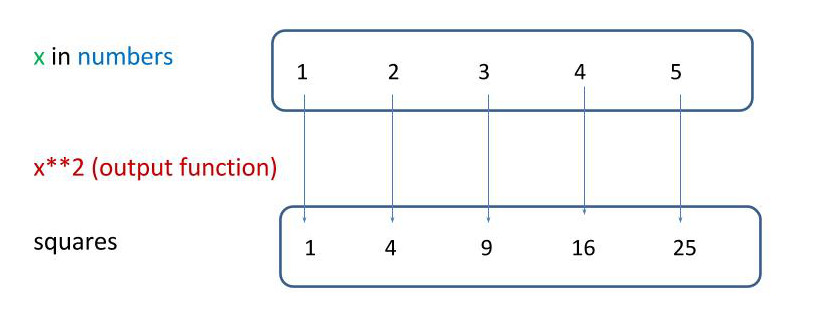
\includegraphics[scale=.6]{mapping}\\
\end{figure}

numbers is the list we are mapping. The interpreter loops through numbers one element at a time, temporarily assigning the value of each element to the variable x. 

Python then applies the function x** 2 and appends that result to the returned list. This function (x**2) is called the output function.

Note that a list comprehension creates a new list.  It does NOT change the original list.

\begin{lstlisting}
>>> print(numbers)

[1, 2, 3, 4, 5]
\end{lstlisting}

The above comprehension is equivalent to

\begin{lstlisting}
squares = []

for x in numbers:

    squares.append(x**2)
\end{lstlisting}

\subsection{Filtering with Comprehension}
List comprehensions may be used to filter items, producing a result that can be smaller than the original list.

To filter a list, we include the if clause at the end of the list comprehension. The expression after the if keyword will be evaluated for each item in the list. If the expression evaluates to True, the item will be included in the output. 

Going back to our comprehension syntax:

[element for variable in iterable if condition]

We can write:

\begin{lstlisting}
>>> numbers = [1, 2, 3, 4, 5]

>>> even_numbers = [x  for x in numbers if x % 2 == 0]

>>> print(even_numbers) 

[2, 4]
\end{lstlisting}

Here we start with the list numbers and we filter it to include only the items that are even in the output list even{\_}numbers.

The above comprehension is equivalent to:

\begin{lstlisting}
even_numbers = []

for x in numbers:

    if x % 2 == 0:        

        even_numbers.append(x)
\end{lstlisting}

We can combine mapping and filtering in one comprehension:

\begin{lstlisting}
>>> numbers = [1, 2, 3, 4, 5]

>>> even_squares = [x**2 for x in numbers if x % 2 == 0]

>>> print(even_squares) 

[4, 16]
\end{lstlisting}

Here we start with the list numbers and we map each item to its square (x**2) but then apply a filter to include only the squares of the even numbers.

The above comprehension is equivalent to:

\begin{lstlisting}
even_squares = []

for x in numbers:

    if x % 2 == 0:

        even_squares.append(x**2)
\end{lstlisting}

Going back to the general syntax of list comprehension:

\begin{lstlisting}
[element for variable in iterable]
\end{lstlisting}

or :

\begin{lstlisting}
[element for variable in iterable if condition]
\end{lstlisting}

It's important to note that the iterable does not have to be a list or a range object.

We can use a dictionary.

\begin{lstlisting}
grades = {'Alice': 95, 'Bob': 85, 'Dan': 90, 'Frank': 88}
\end{lstlisting}

Suppose that we need a list of all students with a grade of A.  We can write:

\begin{lstlisting}
>>> a_students = [student for student in grades if grades[student] >= 90 ] 

>>> print(a_students)

['Alice', 'Dan']
\end{lstlisting}

The above comprehension is equivalent to:

\begin{lstlisting}
a_students = []

for student in grades:

    if grades[student] >= 90:

        a_students.append(student)
\end{lstlisting}

\subsection{Dictionary COmprehension}
A dictionary comprehension is similar to a list comprehension, but we build a dictionary instead of a list. 

The general syntax of a dictionary comprehension is similar to list comprehension with two differences:

We group the expression using curly braces instead of square brackets.
The expression before the 'for' keyword includes both a key and a value, separated by a colon.

\begin{lstlisting}
{key:value for variable in iterable}
\end{lstlisting}

or : 

\begin{lstlisting}
{key:value for variable in iterable if condition}
\end{lstlisting}


\subsubsection{Initializing a dictionary}

Suppose we need to initialize a dictionary, \textit{count}, such as each lower case letter has a corresponding initial count value of 0. We could do that by simply typing all the keys and their value (0) as follows:

\begin{lstlisting}
>>> count = {'a': 0, 'b': 0, 'c': 0, 'd': 0, 'e': 0, 'f': 0, 'g': 0, 'h': 0, 'i': 0, 'j': 0, 'k': 0, 'l': 0, 'm': 0, 'n': 0, 'o': 0, 'p': 0, 'q': 0, 'r': 0, 's': 0, 't': 0, 'u': 0, 'v': 0, 'w': 0, 'x': 0, 'y': 0, 'z': 0} 
\end{lstlisting}

However, this is tedious and error-prone. We could instead use dictionary comprehension to do the same job. 

We’ll also use a constant from the string module to get all our lowercase letters.

\begin{lstlisting}
>>> import string 

>>> string.ascii_lowercase 

'abcdefghijklmnopqrstuvwxyz'

>>> count = {letter:0 for letter in string.ascii_lowercase} 

>>> print(count) 

{'k': 0, 'j': 0, 'i': 0, 'h': 0, 'o': 0, 'n': 0, 'm': 0, 'l': 0, 'c': 0, 'b': 0, 'a': 0, 'g': 0, 'f': 0, 'e': 0, 'd': 0, 'z': 0, 'y': 0, 'x': 0, 's': 0, 'r': 0, 'q': 0, 'p': 0, 'w': 0, 'v': 0, 'u': 0, 't': 0}
\end{lstlisting}

The above comprehension is equivalent to: 

\begin{lstlisting}
count = {} 

for letter in string.ascii_lowercase: 

    count[letter] = 0
\end{lstlisting}

\subsubsection{Mapping}

Now suppose a hypothetical teacher would like to give everyone an extra 2 points on their final grade. We can map an existing dictionary to a new one as follows: 

\begin{lstlisting}
>>> grades = {'Alice': 95, 'Bob': 85, 'Dan': 90, 'Frank': 88} 

>>> new_grades = {student: grades[student] + 2 for student in grades } 

>>> print(new_grades) 

{'Dan': 92, 'Bob': 87, 'Alice': 97, 'Frank': 90} 
\end{lstlisting}

The above comprehension is equivalent to: 

\begin{lstlisting}
new_grades = {} 

for student in grades: 

    new_grades[student] = grades[student] + 2
\end{lstlisting}

\subsubsection{Filtering}

We can also include an if clause in a dictionary comprehension to filter the iterable based on a given expression. 

\begin{lstlisting}
grades = {'Alice': 95, 'Bob': 85, 'Dan': 90, 'Frank': 88} 

>>> a_students = {student: grades[student] + 2 for student in grades if grades[student] >= 90 } 

>>> print(a_students) 

{'Alice': 97, 'Dan': 92} 
\end{lstlisting}

The above comprehension is equivalent to: 

\begin{lstlisting}
a_students = {} 

for student in grades: 

    if grades[student] >= 90: 

        a_students[student] = grades[student] + 2
\end{lstlisting}

\subsubsection{Swapping Keys and Values}

Dictionary comprehension may be used to swap the keys and values of a dictionary. 

\begin{lstlisting}
>>> address_book = {'Alice': '555-1234', 'Bob':'555-1111', 'Carol': '555-2222', 'Daniel':'555-3333'} 

>>> phone_lookup = { address_book[name]: name for name in address_book}

>>> print(phone_lookup) 

{'555-3333': 'Daniel', '555-1111': 'Bob', '555-1234': 'Alice', '555-2222': 'Carol'}
\end{lstlisting}

The above comprehension is equivalent to: 

\begin{lstlisting}
phone_lookup = {} 

for name in address_book: 

    value = address_book[name]

    phone_lookup[value] = name  
\end{lstlisting}

Note that if the values of the dictionary are not unique, the result is not what we may expect: 

\begin{lstlisting}
>>> count = {'the': 300, 'is': 524, 'they': 200, 'an': 300} 

>>> swapped = {count[word]:word for word in count}  

>>> print(swapped)

{200: 'they', 300: 'the', 524: 'is'}
\end{lstlisting}

Because  'the' and 'an' have the same value, only one of them appears in the output dictionary.

Remember that this swapping only works if the values of the dictionary are immutable, like strings or tuples. 

It will NOT work with a dictionary that contains lists. 

\begin{lstlisting}
>>> my_dict = {'a': [1, 2, 3], 'b': 4, 'c': 5} 

>>> {my_dict[key]:key for key in my_dict}

Traceback 

TypeError: unhashable type: 'list'
\end{lstlisting}

\subsection{Set Comprehension}
Sets have their own comprehension as well. The syntax is similar to the syntax for dictionary comprehension and list comprehension. 

\begin{lstlisting}
{element for variable in iterable}
\end{lstlisting}

or :

\begin{lstlisting}
{element for variable in iterable if condition}
\end{lstlisting}

Let’s go back to our example where our task was to identify the students with a grade of A.  We can use the same expression we used with list comprehension but capture the result in a set, instead of a list.

\begin{lstlisting} 
>>> grades = {'Alice': 95, 'Bob': 85, 'Dan': 90, 'Frank': 88}

>>> a_students = {student for student in grades if grades[student] >= 90}

>>> print(a_students)

{'Dan', 'Alice'}
\end{lstlisting}

The above comprehension is equivalent to:

\begin{lstlisting}
a_students = set()

for student in grades:

    if grades[student] >= 90:

        a_students.add(student)
\end{lstlisting}

\section{Python Modules and the Standard Library}
We have already seen how to create and use Python modules.

In the programming assignments, you have created several modules that you have executed directly.  You have also created modules that only included class definitions.  These modules were not executed directly:  they were imported into another module.

In general, a module is a file consisting of Python code. A module can define functions, classes and variables. A module can also include runnable code.

A module allows us to logically organize our Python code. Grouping related code into a module makes the code easier to understand and use.

We can use any Python source file as a module by executing an import statement in some other Python source file or even in the interpreter.

\begin{itemize}
\item import social

\item import car

\item import account
\end{itemize}

The file name is the module name with the  .py appended.

So when our code is saved in the file  'social.py', the corresponding module name is 'social'.

\subsection{Namespace and Scope}
A namespace is a collection of identifiers that belong to a module, to a function, or to a class.

Generally, a namespace holds 'related' things, like all the math functions, or all the date time related behavior.

Each module has its own namespace, so we can use the same identifier name in multiple modules without causing an identification problem.

To access identifiers belonging to a given module that we have imported, we need to prefix the identifier with the module name using the dot notation modulename.identifiername.

We refer to this name as a fully qualified name.

\begin{lstlisting}
>>>import math
\end{lstlisting}

After importing the math module, we can access the sin function from that module by writing: math.sin.

\begin{lstlisting}
>>> math.sin(0)

0.0
\end{lstlisting}

The scope of an identifier is the region of program code in which the identifier can be accessed, or used.

There are three important scopes in Python:

\begin{itemize}
\item Local scope refers to identifiers declared within a function. These identifiers are kept in the namespace that belongs to the function, and each function has its own namespace.

\item Global scope refers to the identifiers declared within the current module.

\item Built-in scope refers to all the identifiers built into Python — identifiers like len and min that can be used without having to import anything, and are (almost) always available.
\end{itemize}

Python uses some precedence rules. The same name could occur in more than one of these scopes, but the innermost, or local scope, will always take precedence over the global scope, and the global scope always gets used in preference to the built-in scope.

We have also seen a variant of the import statement that imports names from a module directly into the importing namespace. 

\begin{lstlisting}
>>> from math import sin
\end{lstlisting}

The sin function has been directly imported into the current namespace and may now be used without being prefixed with math.

\begin{lstlisting}
>>> sin(0)

0.0
\end{lstlisting}

If we prefix it with the module name math, we get an error because the math module itself has not been imported, only the sin function.

\begin{lstlisting}
>>> math.sin(0)

Traceback (most recent call last):

  File "<string>", line 301, in runcode

  File "<interactive input>", line 1, in <module>

NameError: name 'math' is not defined
\end{lstlisting}

The sin function is the only one available.  Other math functions are NOT available.

\begin{lstlisting}
>>> cos(0)

Traceback (most recent call last):

  File "<string>", line 301, in runcode

  File "<interactive input>", line 1, in <module>

NameError: name 'cos' is not defined
\end{lstlisting}

To figure out what names we have access to at a certain point, after some imports, we use the dir function.

\begin{lstlisting}
>>> import account

>>> import math

>>> dir()

['__builtins__', 'account', 'math', 'sys']

>>> from car import Car

>>> dir()

['Car', '__builtins__', 'account', 'math', 'sys']
\end{lstlisting}

These are all the names available in our current namespace, at this time.

It is also possible to import all names from a module into the current namespace by using the following import statement:

\begin{lstlisting}
>>> from math import *
\end{lstlisting}

This provides an easy way to import all the items from a module into the current namespace.  However, this statement should be used sparingly as it it can result in confusion if the same identifier names are used in different modules.

\begin{lstlisting}
>>> dir()

['__builtins__', 'acos', 'acosh', 'asin', 'asinh', 'atan', 'atan2', 'atanh', 'ceil', 'copysign', 'cos', 'cosh', 'degrees', 'e', 'erf', 'erfc', 'exp', 'expm1', 'fabs', 'factorial', 'floor', 'fmod', 'frexp', 'fsum', 'gamma', 'hypot', 'isfinite', 'isinf', 'isnan', 'ldexp', 'lgamma', 'log', 'log10', 'log1p', 'log2', 'modf', 'pi', 'pow', 'radians', 'sin', 'sinh', 'sqrt', 'sys', 'tan', 'tanh', 'trunc']
\end{lstlisting}

\subsection{Module Directory}
We’ve already seen how to use the help function to get help on a module:

\begin{lstlisting}
>>>import math
>>> help(math)
Help on built-in module math:
 
NAME
    math
 
DESCRIPTION
    This module is always available.  It provides access to the
    mathematical functions defined by the C standard.
 
FUNCTIONS
    acos(...)
        acos(x)
        
        Return the arc cosine (measured in radians) of x.
    
    acosh(..
\end{lstlisting}
 
We may also use the built-in function dir to get a list of all the names (variables, functions, classes) that are defined by a given module. 

\begin{lstlisting}
>>> import math
>>> dir(math)
['__doc__', '__loader__', '__name__', '__package__', '__spec__', 'acos', 'acosh', 'asin', 'asinh', 'atan', 'atan2', 'atanh', 'ceil', 'copysign', 'cos', 'cosh', 'degrees', 'e', 'erf', 'erfc', 'exp', 'expm1', 'fabs', 'factorial', 'floor', 'fmod', 'frexp', 'fsum', 'gamma', 'hypot', 'isfinite', 'isinf', 'isnan', 'ldexp', 'lgamma', 'log', 'log10', 'log1p', 'log2', 'modf', 'pi', 'pow', 'radians', 'sin', 'sinh', 'sqrt', 'tan', 'tanh', 'trunc']
\end{lstlisting}

\subsection{The Standard Library}
Python includes a large number of functions, methods and tools and not all of them are available by default. These tools are organized into modules, which make up the Python Standard Library. To use these modules, we have to explicitly import them. 

Here are some of the modules included the standard library. We'll cover the highlighted ones in this course. 

os 
sys
re
math
unittest
urllib
datetime
collections
threading
array
random
tkinter
There are also many third party modules that we may download and import.

Modules are sometimes grouped into packages.

A package is a collection of Python modules: instead of a single file, a package is a directory of Python modules containing an additional {\_}{\_}init{\_}{\_}.py file.

The urllib package is actually a directory with modules organized as follows:

urllib: {\_}{\_}init{\_}{\_} , error, parse, request, response, robotparser

The module name urllib.request designates the submodule request in the package urllib.

\subsection{The sys Module}
The sys module contains functions and variables that provide access to the environment in which the python interpreter runs.  We'll take a look at some of these variables and functions next.

\subsubsection{The sys.argv variable}

One of the most useful and widely used variables in the sys module is the sys.argv variable.  It  holds a list of strings read in from the command line when a Python module is run.   These command line arguments can be used to pass information to a program at the time it is invoked.

We specify the command line arguments when we invoke a Python program from the command line or terminal window.


The general format is:

\begin{lstlisting}
python modulename.py  argument1 argument2 …
\end{lstlisting}

For example:

\begin{lstlisting}
python helloagain.py Bob 5
\end{lstlisting}

The arguments are separated by a space character.

If we want to pass an argument with a space character in it, we use double quotes to enclose it.

python helloagain.py "Bob Smith"  5

The module filename and the arguments are turned into a list of strings and assigned to the argv variable in the sys module. 

The length of the list is at least one.  Even when we don’t explicitly pass any arguments, the module filename is passed to the program.

Let’s demonstrate how sys.argv works by revisiting our hello friend program.

We would like our program to print a customized hello not just once but a certain number of times.  And we don’t want to prompt the user for their name and the number of times they want the message printed, we just want to let them specify that when they invoke the program with the command line arguments:

\begin{lstlisting}
python helloagain.py Bob 5
\end{lstlisting}

The first thing we need to do is to import sys:

We add the following line at the top of our module:

\begin{lstlisting}
import sys
\end{lstlisting}

Inside our module, we now have access to the argument list as sys.argv.

We can check that the correct number of arguments is passed to our program by checking the length of the list: 
\begin{lstlisting}
len(sys.argv).
\end{lstlisting}

Note that the module file name is ALWAYS the first item in that list so if we are expecting 2 arguments, the length of our list will be 3.

We can add some more error checking: if the second argument is NOT a number, we'll issue the appropriate error message.

\begin{lstlisting}
# -----------------------------------------------------------------------------
# Name:        helloagain
# Purpose:     demonstrate command line arguments
#
# Author:      Rula Khayrallah
#
# -----------------------------------------------------------------------------
"""
print a customized hello a given number of times
usage: helloagain.py name number
"""
import sys
def main():
    print ('This is sys.argv:', sys.argv) # for demonstration purposes
    if len(sys.argv) != 3:  #  check for the right number of arguments
        print ('Please try again: helloagain.py name number')
    else:
        name = sys.argv[1]  #  get the name argument
        try:
            number = int(sys.argv[2])  #  get the number argument
        except ValueError:
            print ('Please try again: helloagain.py name number')
        else:   # Print the name the specified number of times
            for i in range (number):
                print ('Hello', name)
if __name__ == '__main__':
    main()
\end{lstlisting}

Note that sys.argv is a list.

\begin{itemize}
\item sys.argv[0] is always the module file name.
\item sys.argv[1] is the first argument specified on the command line after the filename.  Here it is supposed to give us the name.
\item sys.argv[2] is the second argument specified on the command line after the filename.  Here it is supposed to give us the number.
\end{itemize}

Let's test our program from the command prompt or the terminal window:

\begin{lstlisting}
C:\Users\Rula\Documents\CS21A>python helloagain.py Bob  5        

This is sys.argv: ['helloagain.py', 'Bob', '5']

Hello Bob

Hello Bob

Hello Bob

Hello Bob

Hello Bob

sys.argv[0]  is 'helloagain.py'

sys.argv[1] is 'Bob'

sys.argv[2] is '5'
\end{lstlisting}

If we specify too many arguments, we get an error message:

\begin{lstlisting}
C:\Users\Rula\Documents\CS21A>python helloagain.py Bob  5 alice

This is sys.argv: ['helloagain.py', 'Bob', '5', 'alice']

Please try again: helloagain.py name number
\end{lstlisting}

And if the second argument is not a number, we get an error message:

\begin{lstlisting}
C:\Users\Rula\Documents\CS21A>python helloagain.py Bob alice   

This is sys.argv: ['helloagain.py', 'Bob', 'alice']

Please try again: helloagain.py name number
\end{lstlisting}

The sys.path variable:

When we import a module, the Python interpreter searches for it in folders specified in a search path. That search path is stored in the system module sys as the sys.path variable.

To check it out, from the interpreter prompt, we type:

\begin{lstlisting}
>>>import sys

>>> sys.path

['C:\\Program Files (x86)\\JetBrains\\PyCharm Community Edition 3.4.1\\helpers\\pydev', 'C:\\Windows\\SYSTEM32\\python34.zip', 'C:\\Python34\\DLLs', 'C:\\Python34\\lib', 'C:\\Python34', 'C:\\Python34\\lib\\site-packages', 'C:\\Users\\Rula\\Documents\\CS21A']
\end{lstlisting}

Note that sys.path is just a list. 

We can modify it with standard list methods. 

\begin{lstlisting}
>>> sys.path.insert(0,'c:/documents/Rula/CS21A/grading')

>>> sys.path

['c:/documents/Rula/CS21A/grading', 'C:\\Program Files (x86)\\JetBrains\\PyCharm Community Edition 3.4.1\\helpers\\pydev', 'C:\\Windows\\SYSTEM32\\python34.zip', 'C:\\Python34\\DLLs', 'C:\\Python34\\lib', 'C:\\Python34', 'C:\\Python34\\lib\\site-packages', 'C:\\Users\\Rula\\Documents\\CS21A']
\end{lstlisting}

insert(0,…) inserts the folder at the front of the path list.

\begin{lstlisting}
>>> sys.path.append('c:/nosuchdir')

>>> sys.path

['c:/documents/Rula/CS21A/grading', 'C:\\Program Files (x86)\\JetBrains\\PyCharm Community Edition 3.4.1\\helpers\\pydev', 'C:\\Windows\\SYSTEM32\\python34.zip', 'C:\\Python34\\DLLs', 'C:\\Python34\\lib', 'C:\\Python34', 'C:\\Python34\\lib\\site-packages', 'C:\\Users\\Rula\\Documents\\CS21A', 'c:/nosuchdir']
\end{lstlisting}

Note that we have both forward and backward slashes here.  Forward slashes are preferable since they don’t have to be escaped in Python strings.

append() adds the folder to the end of the path list.

Note that changes to sys.path are NOT permanent.  They remain valid only until the current Python process ends or until we exit the current interpreter session.

\subsubsection{sys.exit()}

sys.exit() allows us to exit from the current Python process. 

This is implemented by raising the SystemExit exception.

sys.exit takes an optional argument.  It can be an integer giving the exit status (defaulting to zero), or another type of object. 

If it is an integer, zero is considered successful termination. 

 sys.exit("some error message") is a quick way to exit a program when an error occurs.

Since sys.exit()  only raises an exception, it will only exit the process when the exception is not intercepted.

\subsubsection{Standard Input, Output and Error}

sys.stdin, sys.stdout and sys.stderr  are file objects used for standard input, output and errors.

sys.stdin is used for all interactive input

sys.stdout is used for the output of print statements.

sys.stderr is used for error messages.

Sometimes it is useful to redirect the tracebacks from exceptions to a file that will be examined later.

We can do that by adding the following:

\begin{lstlisting}
    sys.stderr =  open ('errors.txt', 'w')
\end{lstlisting}

The file errors.txt will now contain all the exceptions tracebacks.

\section{Regular Expressions}
\subsection{What are Regular Expressions?}

Regular expressions, also called REs, regexes, or regex patterns are a highly specialized programming language embedded inside Python and made available through the re module.

Regular expressions offer a standardized way of searching, replacing, and parsing text with complex patterns of characters. 

Using Regular Expressions, we specify the rules or the pattern for the set of possible strings that we want to match.  This set might contain English sentences, e-mail addresses, or anything else we are interested in. 

We can then ask questions such as "Is there a match for the pattern anywhere in this string?"

We can also use REs to modify a string or to split it apart in various ways.

\subsection{String Methods or Regular Expressions?}
It is important to remember that in Python, strings have several built-in methods for searching and replacing.

\begin{lstlisting}
>>> text='Hello!  Welcome to CS21A!'

>>> print(text.find('!'))

5

>>> print(text.replace('!', '.'))

Hello.  Welcome to CS21A.

>>> print(text.replace('Hello', 'Hi'))

Hi!  Welcome to CS21A!

>>> print('.'.join(['filename', 'txt']))

filename.txt
\end{lstlisting}

The find method above returns the lowest index in text where the exclamation mark is found. 

The replace method above returns a copy of text where all the occurrences of the exclamation point have been replaced by a period.

The join method above returns a concatenation of filename and txt with '.' as the separator.

So before trying to solve a given problem with regular expressions, it is important to check if that task can be accomplished with the string methods. These are simple and easy to use.

When we have to use a lot of different string methods with \textit{if} statements to handle special cases, it is an indication that we may need to move on to regular expressions.

\subsection{Regular Expressions with Pythex}
Before we look at the available functions in the re module in Python let’s get a hands-on introduction to the regular expression syntax.

One option to quickly test our regular expressions before including them in a program is to use the Pythex website.

Note that Pythex does not work with Internet Explorer.  Make sure you use Firefox or Chrome when you access it.

So what are we testing with the regular expressions?

The idea is that we have a string and we are looking for a certain pattern in that string.

The pattern may be an email address, of the form: something@something.something
Or a phone number of the form:  (nnn) nnn-nnnn
With Pythex we specify a regular expression (which is really a pattern) and a string.  Pythex displays a match in case there is one.

\subsubsection{Matching characters}

We’ll start with a trivial example:  most letters and characters will simply match themselves.  

'Hello' is the regular expression and the text we are examining is 'Hello World'.  The regular expression 'Hello' matches 'Hello' in 'Hello World'.

Instead of 'Hello', let’s put in 'hello' for the regular expression.  There is no match.

\subsubsection{Metacharacters}

Some characters are special metacharacters, and don’t match themselves. 

Instead, they indicate that some other thing should be matched, or they affect other parts of the regular expression by repeating them or changing their meaning. 

Here’s a complete list of the metacharacters:

\begin{lstlisting}
. ^ $ * + ? { } [ ] \ | ( )
\end{lstlisting}

We'll take a look at each of them next.

\subsubsection{[] -  set of characters}
The square brackets are used to specify a set of characters that we want to match.

Characters can be listed individually as in [abc]. 

We can also specify a range of characters as two characters separated by a hyphen: [a-c]. 

So [abc] will match any of the characters a, b, or c; this is the same as [a-c]. If we want to match only lowercase letters, we use [a-z].

[0-9] will match 0, 1, 2, 3, 4, 5, 6, 7,8 and 9.

[A-Z] will match only upper case characters.

Note that everything within the square bracket, represents one character NOT a sequence of characters.

Matching H[ello]

So specifying H[ello] means match: 

He

or

Hl 

or 

Hl

or

Ho

 

Metacharacters are not active inside the square brackets []. For example, [akm\$] will match any of the characters 'a', 'k', 'm', or '\$'; '\$' is usually a metacharacter, but inside the brackets, it’s just the character \$.

\subsubsection{Negating the Set}
We can match the characters not listed within the set by complementing (negating) the set. This is indicated by including a '\^' as the first character of the set.  


\subsubsection{ . - Any character}
The dot . matches any character except a newline character.  

There is a flag that can be set (DOTALL) so that the dot will match even a newline. 

The dot is often used when we want to match 'any character'.

\subsubsection{\^ \$  - beginning and end} 
\^ matches the beginning of the string or if the MULTILINE flag is set the beginning of each line.  Note that \^ has a different meaning (not) when it is inside square brackets.

\$ matches the end of the string or if the MULTILINE flag is set the end of each line.

First and Last Characters:
\^. will match the first character.

.\$ will match the last character.

\subsubsection{Repeating Characters: *, + and ?}
* indicates that the previous character can be matched zero or more times.

+ indicates that the previous character can be matched one or more times.

? indicates that the previous character can be matched zero or one time.  In other words, it indicates an optional character.

Repetitions such as * are greedy.  When repeating a regular expression, the matching engine will try to repeat it as many times as possible.

So o*ps on  the right above matches oooops not ops or oops or ooops.

Sometimes we want the repetition to be non greedy.  Suppose we are trying to extract double quoted strings from a text.  Using ".*" does not work – it just matches everything from the first " to the last ".

To fix that we add a ? after  the * to make the match non-greedy: ".*?"

+ indicates that the previous character can be matched one or more times.

We’ve  seen how to use the question mark character after * to make the repetition non-greedy.

We can also use the question mark character (without *) to indicate  that the previous character is optional. 

The question mark character, ?, matches either once or zero times.  It can be used below to indicate that the 'u' is optional in colors (or colours).

\subsubsection{Repeating Characters: {}}
{m} means repeat the previous character(s) exactly m times.

[0-9]{3} means repeat the digit [0-9] exactly 3 times.

\subsubsection{{m,n} means repeat the previous character(s) m to n times}

o{2,4} means repeat the o character between 2 and 4 times.

Note that when we write:

bo{2,4}

The {2,4} applies to the o only.

To repeat a sequence of characters, we use parentheses as follows:

(ho){2,4}

The {2,4} now applies to the 'ho'.

Repeating a group of characters with parentheses

\subsubsection{Or: |}

The vertical bar | indicates a choice.  

\subsubsection{Parentheses - ()}
The parentheses may be used to group parts of the expression together to indicate precedence like in recogni(z|s)e or (ho){2,4}.

Parentheses also capture the matched element into a variable (capture group) that may be used later.

Here we have captured two groups: 

([0-9]{3}) is the first one and  ([0-9]{3}-[0-9]{4}) is the second

The two groups appear now under Match captures.

Sometimes we need the parentheses to indicate precedence but we don’t really want to capture the group.

We can add ?: inside the parentheses to disable capturing.

Here we need the parentheses around the (s|z) for precedence but we only want to capture the whole word.  So we use (recogni(?:s|z)e).

\begin{lstlisting}
Escape Character: \
The backslash may be used as an escape character and it means: treat whatever metacharacter comes after it as a literal.  

For example in an email address pattern, we want to use the dot to actually denote a dot, not any character.  We can write:


 ([a-z]+@[a-z]+\.[a-z]+)


The backslash may also be used to signal a special character.

Here are some of the more useful special characters:


\d matches any decimal digit.  This is the same as [0-9].
\item \D matches any non-digit character. This is the same as [^0-9].
\item \s matches any whitespace character.
\item \S matches any non-whitespace character.
\item \w matches any word character – that is any alphanumeric  character  or the underscore.  This is the same as [a-zA-Z0-9_].
\item \W matches any non-word character. This is the same as  [^a-zA-Z0-9_].
\item \b matches a word boundary.  For example  \bred\b will match red in ' red?' or '-red,' but not 'redo' or 'credit'. 
These special characters can be used inside []. 


For example, [\s,.] will match any whitespace character, or ',' or '.'.

Note that each of these will match only one character.

When we actually want to match a backslash, we have to escape it – precede it with another backslash:  \\ .  The first \ tells the re engine to treat the second \ as a literal (not as a metacharacter). 

escaping the backslash

So c:\\d will match c:\documents and not c:\\documents.

Suppose that we want to capture email addresses that include digits and  the & character:

Alice:  alice123@foothill.edu

Bob:  bob&carol@fhda.edu

The pattern that we have used previously  ([a-z]+@[a-z]+\.[a-z]+) will not work.

 

Using [a-z] excludes the 123 in alice123 and the & in bob&carol. 

Using [a-z] excludes the 123 in alice123 and the & in bob&carol. 

Instead of [a-z] we can use \S - any non whitespace character. 

Using \S works
\end{lstlisting}

\subsection{The RE Module}
To use regular expressions in Python, we need the re module.

We'll take a look at the following functions available in the re module: match, search, findall and finditer.

To use these functions, we need to import the module.

import re

To call each function, we need to prefix it with the module name:

re.match

re.search

re.findall

re.finditer

\subsection{Raw Strings}
Before we go on to the specific functions in the re module, we need to talk about raw strings in Python.

Remember that regular expressions use the backslash ('\') for special characters to allow metacharacters to be used without invoking their special meaning.

To write one backslash inside a regular expression, we have to write '\\'. The first backslash tells us that the second backslash has no special meaning.

Python also uses the backslash in strings as an escape character.

To write one backslash inside a Python string, we also have to 'escape' it:  we write '\\'.  The first backslash tells Python to use the second backslash as is.

As a result if we use Python strings to write a pattern to match one backslash, we have to write '\\\\' as the pattern string: 

The regular expression must be \\ (that’s what we would write in Pythex). 
But then each backslash must be expressed as \\ inside a regular Python string.
The solution is to use Python’s raw string notation for regular expressions. Backslashes are not handled in any special way in a raw string.

A raw string is a string prefixed with r such as: 

\begin{lstlisting}
my_raw_string = r"hello"
\end{lstlisting}

In Python it is recommended to use this raw string notation for all patterns.

\subsection{re.match and Match Objects}
The re.match function is used to determine if there is a match at the beginning of the string.

Syntax:  re.match(pattern, string, flags=0)

The function returns a match object on success, None on failure. 

Here's an example:

\begin{lstlisting}
>>> import re

>>> my_pattern  = r'Hello'

>>>print(re.match(my_pattern, 'Hello World!'))

<_sre.SRE_Match object; span=(0, 5), match='Hello'>

>>> print (re.match(my_pattern, 'Hi Class! Hello World!'))

None
\end{lstlisting}

The match function looks for a match at the beginning of the string.  Since Hello is not at the beginning in the above example, there is no match and None is returned.

\subsubsection{What’s a match object and how can we access it?}
The group method may be invoked on the match object to return the substring that was matched.

\begin{lstlisting}
>>> import re

>>> my_pattern  = r'Hello'

>>> my_match = re.match(my_pattern, 'Hello World!')

>>> print(my_match.group())

Hello
\end{lstlisting}

The \textit{start} and \textit{end} methods  are also available on the match object: they return the starting and ending index of the match.

The \textit{span} method returns both the start and end indexes in a single tuple. 

Since the match function only checks if the pattern specified matches at the start of a string, start will always return zero when invoked on a match object returned by match.

\begin{lstlisting}
>>> my_pattern  = r'Hello'

>>> my_match = re.match(my_pattern, 'Hello World!')

>>> print(my_match.group())

Hello

>>> print(my_match.start())

0

>>> print(my_match.end())

5

>>> print(my_match.span())

(0, 5)
\end{lstlisting}

\subsection{RE Flags}
The re module functions support a flag parameter.  That parameter can take on one or more values.

re.IGNORECASE:   This flag indicates case-insensitive matching.  

\begin{lstlisting}
>>> my_pattern  = r'hello'

>>> my_match = re.match(my_pattern, 'Hello World!', re.IGNORECASE)

>>> print(my_match.group())

Hello
\end{lstlisting}

re.MULTILINE:  When this flag is specified, the metacharacter '\^' matches at the beginning of the string and at the beginning of each line in a multi-line string.  Similarly the meta character '\$' matches at the end of the string and at the end of each line in a multi-line string.

Without this flag , '\^' matches only at the beginning of the string, and '\$' only at the end of the string.

re.DOTALL:  This flag makes the '.' metacharacter match any character at all, including a newline.

Without this flag, '.' will match anything except a newline.

re.VERBOSE:  This flag allows us to write regular expressions that look nicer. Whitespace within the pattern is ignored, except inside[]  or preceded by a backslash, and, when a line contains a '\#' characters from the leftmost such '\#' through the end of the line are ignored.

To use more than one flag in a single function call, we can use |.

\begin{lstlisting}
>>> my_match = re.match(r'h.e', 'H\nello', re.IGNORECASE|re.DOTALL)
>>> print(my_match.group())
H
e
\end{lstlisting}

Here we are looking for an h and an e separated by any character (including a new line).

\subsection{re.search}
The re.search function is used to determine if and where the regular expression pattern produces a match at any location in a given string.

Syntax: re.search(pattern, string, flags=0)

The function scans through the string looking for a location where the regular expression pattern produces a match, and returns a corresponding match object. The function returns None if there is no match.

Here again we may invoke the group, start, end and span methods  on the match object.

\begin{lstlisting}
>>> my_pattern  = r'Hello'

>>> my_match = re.search(my_pattern, 'Hi Class! Hello Everyone! Hello World!')

>>> print(my_match.group())

Hello

>>> print(my_match.start())

10

>>> print(my_match.end())

15

>>> print(my_match.span())

(10, 15)
\end{lstlisting}

Note that the search function only finds the first occurrence of the pattern in the string.

What if there is no match?

We should not invoke the group, start, end or span methods unless we know for sure that the match object exists and that the search or match functions did not return None.  So usually, we add an if statement as follows:

\begin{lstlisting}
my_pattern  = r'Hello'

my_match = re.search(my_pattern, 'Hi Class! Hello Everyone! Hello World!')

if my_match:

    print('Match found: ', my_match.group())

else:

    print('No match')
\end{lstlisting}

\subsection{re.findall}
We noted that search will only find the first occurrence of the pattern in the string.  

To find all the occurrences, we can use the findall function.

Syntax:  re.findall(pattern, string, flags=0)

The function finds all non-overlapping substrings where the pattern matches, and returns them as a list of strings. 

The string is scanned left-to-right, and matches are returned in the order found.

Here's an example:

\begin{lstlisting}
>>> email_pattern = r'(\S+@\S+\.\S+)'

>>> text = '''Alice:     alice123@foothill.edu    

…                Bob:    bob&carol@fhda.edu'''

>>> print(re.findall(email_pattern, text))

['alice123@foothill.edu', 'bob&carol@fhda.edu']
\end{lstlisting}

We'll see in an upcoming section that findall sometimes returns a list of tuples instead of a list of strings.

\subsection{re.finditer}
The finditer function may also be used to find all substrings where the pattern matches. 

Syntax: re.finditer(pattern, string, flags=0)

The function returns an iterator yielding match objects  over all non-overlapping matches. 

This iterator provides sequential access to the  match objects.  We can iterate over it with a for loop.

The string is scanned left-to-right, and matches are returned in the order found.

Here's an example:

\begin{lstlisting}
email_pattern = r'(\S+@\S+\.\S+)'

text = '''Alice: alice123@foothill.edu

             Bob:   bob&carol@fhda.edu'''

for match in re.finditer(email_pattern, text):

        print (match.group())

alice123@foothill.edu

bob&carol@fhda.edu
\end{lstlisting}
\subsection{Capture Groups}
When invoked on the match object the group method may be used to return one or more subgroups of the match.

Remember that parentheses capture the matched element into a group.

Going back to our previous example, let's say we are interested in both the name and the email address.  We can write our regular expression as follows:

\begin{lstlisting}
([a-z]+):\s+(\S+@\S+\.\S+)
\end{lstlisting}

\begin{lstlisting}
([a-z]+) 
\end{lstlisting}
corresponds to the name and 
\begin{lstlisting}
(\S+@\S+\.\S+)
\end{lstlisting} corresponds to the email address

We have two capture groups here: the name and the email address.

We also have two matches:  one corresponding to Alice and the other corresponding to Bob.

Going back to Python, we would write our code as follows:

\begin{lstlisting}
my_template = r'([a-z]+):\s+(\S+@\S+\.\S+)'

addresses = '''Alice: alice123@foothill.edu

                         Bob:   bob&carol@fhda.edu'''

my_match = re.search(my_template,addresses,  re.IGNORECASE)

if my_match:

        print(my_match.group())

Alice: alice123@foothill.edu
\end{lstlisting}

The group method, with no arguments (or 0), returns the whole match.

To capture the subgroups separately, we write:

\begin{lstlisting}
my_template = r'([a-z]+):\s+(\S+@\S+\.\S+)'

addresses = '''Alice: alice123@foothill.edu

                         Bob:   bob&carol@fhda.edu'''

my_match = re.search(my_template, addresses,  re.IGNORECASE)

if my_match:

        print(my_match.group())

        print ('Name: ',  my_match.group(1))

        print ('Email address: ', my_match.group(2))
\end{lstlisting}

And here's the corresponding output:

\begin{lstlisting}
Alice: alice123@foothill.edu

Name:  Alice

Email address:  alice123@foothill.edu
\end{lstlisting}

group(1) returns the first subgroup.

group(2) returns the second subgroup.

To capture ALL the names and email addresses, we may use the finditer function and iterate over the matches as follows:

\begin{lstlisting}
my_template = r'([a-z]+):\s+(\S+@\S+\.\S+)'

addresses = '''Alice: alice123@foothill.edu

                      Bob:   bob&carol@fhda.edu'''

all_matches = re.finditer(my_template, addresses, re.IGNORECASE)

for my_match in all_matches:

        print(my_match.group())

        print ('Name: ',  my_match.group(1))

        print ('Email address: ', my_match.group(2))
\end{lstlisting}

And here's the corresponding output:

\begin{lstlisting}
Alice: alice123@foothill.edu

Name:  Alice

Email address:  alice123@foothill.edu

Bob:   bob&carol@fhda.edu

Name:  Bob

Email address:  bob&carol@fhda.edu
\end{lstlisting}

We can also use the findall function.  It will return a list of tuples of match groups as follows:

\begin{lstlisting}
my_template = r'([a-z]+):\s+(\S+@\S+\.\S+)'

addresses = '''Alice: alice123@foothill.edu
 
                      Bob:   bob&carol@fhda.edu'''
 
all_matches = re.findall(my_template, addresses, re.IGNORECASE)
 
for my_match in all_matches:
 
        print(my_match)  # my_match is a tuple
 
        print ('Name: ',  my_match[0])  # the first tuple item is the first group
 
        print ('Email address: ', my_match[1])  # the second tuple item is the second group
\end{lstlisting}
 
Here's the corresponding output:
\begin{lstlisting}
('Alice', 'alice123@foothill.edu')

Name:  Alice

Email address:  alice123@foothill.edu

('Bob', 'bob&carol@fhda.edu')

Name:  Bob

Email address:  bob&carol@fhda.edu
\end{lstlisting}

\subsection{Compiling Regular Expressions}
 It is important to note that all the re functions we have encountered so far take a string parameter as the regular expression pattern.

It is also possible to 'compile' that pattern into a regular expression object and then invoke the corresponding methods on that object to search a given text.

Here's an example.  

\begin{lstlisting}
>>>compiled_pattern = re.compile('H')

>>>compiled_pattern.match('Hello World!')

<_sre.SRE_Match object; span=(0, 1), match='H'>
\end{lstlisting}

The above is equivalent to the code below:

\begin{lstlisting}
>>> re.match('H', 'Hello World!')

<_sre.SRE_Match object; span=(0, 1), match='H'>
\end{lstlisting}

Compiling the pattern is a common practice in other programming languages to improve performance or because it is the only available way to use regular expressions.

However because Python automatically compiles the patterns used with the re functions and stores them in the cache, there is usually no advantage in explicitly compiling our patterns first.

In this course, we'll use the re functions on the string patterns without compiling them.

\section{The urllib Package}
\subsection{Web Background and Terminology}
HTTP (short for Hypertext Transfer Protocol) is the message protocol that supports the world wide web. It specifies the format of messages exchanged between a client, such as a web browser, and a web server.

Web browsers use the HTTP format to request pages from a web server, and web servers use the HTTP format to send back their responses.

HTTP is a fixed format for communication:  it includes specific request and response headers. 

An HTTP request also includes a URL.

The URL (Uniform Resource Locator), also known as web address, is the string that constitutes a reference to the 'resource' that is requested.

In web browsers, the URL of a web page is displayed on top inside an address bar.  The following are examples of urls:

http://www.foothill.edu/

https://etudes.org/

The urllib package includes several modules for working with URLs:

urllib.request: for opening and reading URLs

urllib.error: contains the exceptions raised by  urllib.request.

urllib.parse  for parsing URLs.

urllib.robotparser  for parsing robots.txt files.

\subsection{urllib.request}
The urllib.request module supports fetching and reading URLs. 

It includes a urlopen function  that allows us to 'open' web pages as if they were files.

urlopen takes the address of the page we want, and returns a file-like object that we can just read to get the full contents of the page. 

The read method on that file-like object always returns bytes, not a string.

To get a string, we need to determine the character encoding and explicitly convert it to a string.

Each module in the urllib package has to be imported individually.

\begin{lstlisting}
>>> import urllib.request 
\end{lstlisting}

We have to use the fully qualified name of urlopen.

\begin{lstlisting}
>>> url_file = urllib.request.urlopen('http://www.psme.foothill.edu') 
\end{lstlisting}

One way to look at this:  we are the client here.  urllib is sending an HTTP request on our behalf to the server at psme.foothill.edu.  The server is sending back a response…

And another way to look at it:  we are just opening a remote file-like object.

Putting it together, we write:

\begin{lstlisting}
>>> import urllib.request 

>>> url_file = urllib.request.urlopen('http://www.psme.foothill.edu') 

>>> print(type(url_file))

<class 'http.client.HTTPResponse'>
\end{lstlisting}

This is the HTTP response to our request.  It is also a file-like object that we can 'read':

\begin{lstlisting}
>>> page = url_file.read()
\end{lstlisting}

We invoke the read method on that file-like object and save its content into a variable.  page is just an arbitrary variable name.   

\begin{lstlisting}
>>> print(type(page))

<class 'bytes'>
\end{lstlisting}

However when we read that file-like object, we get bytes, not a string.

\begin{lstlisting}
>>> print(page)

b'<!DOCTYPE html>\n<!--[if IE 6]>\n<html id="ie6" lang="en-US">\n<![endif]-->\n<!--[if IE 7]>\n<html id="ie7" lang="en-US">\n<![endif]-->\n<!--[if IE 8]>\n<html id="ie8" lang="en-US">\n<![endif]-->\n<!--[if !(IE 6) | !(IE 7) | !(IE 8)  ]><!-->\n<html lang="en-US">\n<!--<![endif]-->\n<head>\n<meta charset="UTF-8" />\n<meta name="viewport" content="width=device-width" />…
\end{lstlisting}

We can decode the bytes to get a string.  The charset here indicates a UTF-8 encoding.

\begin{lstlisting}
>>> decoded_page = page.decode('UTF-8')

>>> print(decoded_page)

<!DOCTYPE html>\n<!--[if IE 6]>
<html id="ie6" lang="en-US">
<![endif]-->
<!--[if IE 7]>\n<html id="ie7" lang="en-US">
<![endif]-->
<!--[if IE 8]>
<html id="ie8" lang="en-US">
<![endif]-->
<!--[if !(IE 6) | !(IE 7) | !(IE 8)  ]><!-->
<html lang="en-US">
<!--<![endif]-->
<head>
<meta charset="UTF-8" />
<meta name="viewport" content="width=device-width" />…
\end{lstlisting}

Note that the page we printed is an HTML page.

HyperText Markup Language (HTML) is the main markup language for creating web pages that can be displayed in a web browser.

One way to get an idea about HTML is to look at the source for web pages that you commonly use.  In most browsers, you can right click on a web page (or CTRL click on a MAC OS) and select 'View page source' to see the corresponding HTML source.

Let's do that with the web page at http://www.foothill.edu/counseling/.

We first point our browser to http://www.foothill.edu/counseling/.  We then right click  on the page and select 'View page source'.  Scrolling down the page, we take a closer look at the text.  Here's a sample of what we see (at the time this module is written):

\begin{lstlisting}
<div class="colhead">Our Mission</div>
<div style='margin-left:10px;'>
The mission of the Counseling Division is to help students make appropriate and 
successful educational decisions, set achievable and realistic goals, adjust to 
changing roles in a global society and resolve academic, transfer and career 
concerns that can interfere with the ability to succeed in their college experience.
</div>
 
<div class="linespace">&nbsp;</div>
<div class="colhead">Main Campus Location</div>
\end{lstlisting}
 
An HTML document contains content (words, images, audio, video) as well as special instructions to the browser for displaying each type of content. The instructions are included inside tags. Tags are enclosed in angle brackets (< >).  When we look at the web page in the browser, we only see the content that is outside the tags.  That content is 'rendered' by the browser based on the special instructions given inside the tags.

However when we open the url with urllib.request.open and read it, we get both the instructions and the content.

To analyze or compile information found at a given url, we usually need to look only at the content found outside the tags.  That's what we'll do in our aggregator assignment.

\subsubsection{Closing the URL}

We said that urllib.request.urlopen returns a file-like object.

Once we have read that file, we need to close it.

There are two ways to do that.

We can invoke the close method on the file-like object url{\_}file.

\begin{lstlisting}
>>> url_file = urllib.request.urlopen('http://www.psme.foothill.edu') 

>>> page = url_file.read()

>>> url_file.close()
\end{lstlisting}

Or better yet, just like with files, we can use the with statement:

\begin{lstlisting}
>>>with urllib.request.urlopen('http://www.psme.foothill.edu') as url_file:

            page = url_file.read()
\end{lstlisting}

And the file-like object is automatically closed when we get out of the with indented block.

\subsubsection{Capabilities and Limitations}

The urllib.request module follows http redirects but treats them all as 'temporary' redirects.

It handles some common forms of authentication: basic and digest.

It does not support caching or compression.

\subsection{urllib.parse}
The urllib.parse module defines a standard interface to manipulate URL strings.

It includes functions to:
\begin{itemize}
\item break up a URL into its components (urlparse).
\item combine the components back into a URL string.
\item convert a relative URL to an absolute URL (urljoin).
\end{itemize}

It supports several URL schemes including http, https, ftp and file.

The general structure of an absolute URL is:

\begin{lstlisting}
scheme://hostname/path;parameters?query#fragment
\end{lstlisting}

Consider the following url:

\begin{lstlisting}
http://www.foothill.edu/news/newsfmt.php?sr=2&rec_id=3200
\end{lstlisting}

The scheme identifies the protocol to be used.  The scheme in the example above is  http. 

The hostname is also known as the domain (or network location.)  The hostname in the example above is  www.foothill.edu.   

The path refers to the specific resource within the host that we want to access.  The path in the example above is  /news/newsfmt.php. 

There are no parameters specified here.     

The query is usually a string of name and value pairs that will be passed to the resource.  The query here is 
\begin{lstlisting}
sr=2&rec_id=3200.
\end{lstlisting}

There is no fragment specified here.

\subsubsection{urllib.parse.urlparse}
The urllib.parse.urlparse function  breaks up a URL into six components. 

Each component is a string, possibly empty.

\begin{lstlisting}
>>> import urllib.parse

>>> url = 'http://www.foothill.edu/news/newsfmt.php?sr=2&rec_id=3200'

>>> o = urllib.parse.urlparse(url)

>>> print(type(o))

<class 'urllib.parse.ParseResult'>

>>> print(o)

ParseResult(scheme='http', netloc='www.foothill.edu', path='/news/newsfmt.php', params='', query='sr=2&rec_id=3200', fragment='')
\end{lstlisting}

urlparse returns an object with 6 components.  We can access each of these components by its name as follows:

\begin{lstlisting}
>>> print(o.scheme)

http

>>> print(o.hostname)

www.foothill.edu

>>> print(o.path)

/news/newsfmt.php

>>> print(o.params)  # no parameters here so nothing is printed

>>> print(o.query) 

sr=2&rec_id=3200
\end{lstlisting}

\subsubsection{Absolute and Relative URLs}
Absolute and relative URLs are similar to absolute and relative file names.

Absolute URLs contain more information but relative URLs are convenient and more portable.

Relative URLs are relative to a base URL.  The base URL is the URL we are currently at.

We must use absolute URLs when referring to links on different servers.

Absolute url: http://www.foothill.edu/counseling/

Relative url:  counseling/

\subsubsection{urllib.parse.urljoin}
The urllib.parse.urljoin  function converts a relative URL to an absolute URL given a 'base URL'.  

Let's see how it works with an example.  Suppose we are on the Foothill URL:

\begin{lstlisting}
http://www.foothill.edu/contact.php
\end{lstlisting}

If we look at the source for that page, we see several 'links'.

Links in HTML are stored as attribute values on various kinds of tags.

Let’s just consider links contained in <a> tags. 

<a> tags have an attribute named href that contains the linked URL.

On that page, here are some of the <a> tags we see:

\begin{lstlisting}
<a href="campuslife/">Campus Life</a>

<a href="http://www.foothill.edu/privacy.php">Privacy Policy</a>
\end{lstlisting}

As you can see, one of these URLS is absolute and one is relative.

Let’s try to construct the absolute URLs for each of them.  

Remember that since all these links are from http://www.foothill.edu/contact.php , that URL is my base.

The syntax of urljoin is as follows:

\begin{lstlisting}
urllib.parse.urljoin(base, url)

>>> import urllib.parse 

>>> url = 'campus_life/'

>>> base = 'http://www.foothill.edu/contact.php'

>>> abs_url = urllib.parse.urljoin(base, url)

>>> print(abs_url)

http://www.foothill.edu/campuslife/
\end{lstlisting}

urljoin works even if we give it an absolute url.  It recognizes it as an absolute and returns it as it is.

This is convenient because we don’t have to do  any pre-processing before we call urljoin.  We can call it with any url (absolute or relative) that we encounter and be certain that we are getting back an absolute url.

\begin{lstlisting}
>>> url = 'http://www.foothill.edu/privacy.php'

>>> abs_url = urllib.parse.urljoin(base, url)

>>> print(abs_url)

http://www.foothill.edu/privacy.php
\end{lstlisting}

\subsection{urllib.error}
The urllib.error module defines the  exception classes raised by urllib.request.

urllib.error.HTTPError – subclass of URLError
urllib.error.ContentTooShortError – subclass of URLError
Note that when handling these exceptions, we need to provide their fully qualified name.

Example 1:
\begin{lstlisting}
import urllib.request
import urllib.error
 
def main():
    url = 'http://nosuchurl.edu'
    try:
        with urllib.request.urlopen(url) as url_file:
            text= url_file.read().decode('UTF-8')
    except urllib.error.URLError as url_err:
        print('Error opening url: ', url, url_err)
 
if __name__ == '__main__':
    main()
Error opening url:  http://nosuchurl.edu (Links to an external site.) <urlopen error [Errno 8] nodename nor servname provided, or not known>
\end{lstlisting}

Example 2:
In this example, we combine two steps in our try statement:  reading the url and decoding it.  To make sure we also catch a decoding exception, we add an except clause as follows:

\begin{lstlisting}
import urllib.request
import urllib.error
def main():
    url = 'http://nosuchurl.edu'
    try:
        with urllib.request.urlopen(url) as url_file:
            text= url_file.read().decode('UTF-8')
    except urllib.error.URLError as url_err:
        print('Error opening url: ', url, url_err)
    except UnicodeDecodeError as decode_err:
        print('Error decoding url: ', url, decode_err)  
        
if __name__ == '__main__':
    main()    
\end{lstlisting}

\subsection{Polite Crawling}
A web crawler is a program that systematically browses the web to extract information.  Search engines use web crawlers to update their indexes of web content.  Web crawlers are also used for scraping the web for contact information (spamming) or online price comparison or news compilation, etc…

Web crawlers  can disrupt networks and Web servers.  If a crawler sends multiple requests to one server and downloads large files, the server’s performance will be affected, especially if there are several crawlers. 

A partial solution to these problems is the robots exclusion protocol, also known as the robots.txt protocol.  It is a standard for administrators to indicate which parts of their web servers should not be accessed by crawlers.

Web site administrators use the robots.txt file to give instructions about their site to web crawlers.  It works likes this: a crawler wants to visit a URL, say domain/welcome.html.  Before it does so, it checks for some rules provided in the file domain/robots.txt.  If the robots.txt file exists for that domain, it then reads it to figure out what it is allowed to crawl.

A polite web crawler tries to comply with the robots exclusion protocol and not crawl web sites if rules in the server's robots.txt file disallow crawling.

The robots.txt file contains the instructions in a specific format.  

Let's take a look at the robots.txt file for www.foothill.edu.

\begin{lstlisting}
http://www.foothill.edu/robots.txt

User-agent: * 
Disallow: /cms/ 
Disallow: /cgi/ 
Disallow: /cgi-bin/ 
Disallow: /support/ 
User-agent: dotbot 
Disallow: /
\end{lstlisting}

User-agent is used to identify the crawler. 

dotbot is an e-commerce crawler and is asked not to crawl foothill.edu.

All other crawlers (*) are asked not to crawl cms, cgi, cgi-bin and support.

Here's the robots.txt file for facebook.com.

\begin{lstlisting}
http://facebook.com/robots.txt

User-agent: Googlebot 
Disallow: /ac.php 
Disallow: /ae.php 
Disallow: /ajax/ 
Disallow: /album.php 
Disallow: /ap.php 
Disallow: /autologin.php 
…
User-agent: msnbot 
Disallow: /ac.php 
….
User-agent: * 
Disallow: /
\end{lstlisting}

\subsection{urllib.robotparser}
The urllib.robotparser module answers questions about whether or not a particular user agent can (politely) fetch a URL on a given web site.

Here's an example:

We first import the module:

\begin{lstlisting}
>>> import urllib.robotparser
\end{lstlisting}

Instantiate a RobotFileParser object:

\begin{lstlisting}
>>> rp = urllib.robotparser.RobotFileParser() 
\end{lstlisting}

Set the URL to the robots.txt file corresponding to the domain:

\begin{lstlisting}
>>> rp.set_url("http://foothill.edu/robots.txt") 
\end{lstlisting}

Read the robots.txt file:

\begin{lstlisting}
>>> rp.read() 
\end{lstlisting}

Answer 'can fetch' questions for various user agents: 

\begin{lstlisting}
>>> print(rp.can_fetch("*", "http://foothill.edu/campuslife/"))

True

>>> print(rp.can_fetch("*","http://www.foothill.edu/support/"))

False
\end{lstlisting}

\section{GUI}
\subsection{What's a GUI?}
A Graphical User Interface is an interface that lets us use icons, toolbars, buttons and menus to achieve tasks.  We point, click, drag, select and the corresponding command is executed.

By contrast, a command line interface is an interface that is text based:  we type in our commands one line at a time.

Python provides several third party frameworks for developing graphical user interfaces. 

Tkinter is the standard GUI library for Python.  It comes bundled with Python.  It offers a fast and easy way to create GUI applications.   It provides a powerful object-oriented interface to the Tk GUI toolkit.

IDLE is a Tkinter GUI.

In this course we'll use Tkinter to illustrate GUI programming in Python.

\subsection{Event-Driven Programming}
GUI applications are event driven. They sit and wait for events to happen.

Events can come from various sources, including key presses and mouse clicks by the user.

When a significant event occurs, they handle it then go back to waiting for the next event.

The following entities are associated with a given event:

The event type (or event name) describes the event:  is it a mouse click, a character input?

The event target is the object on which the event happened:  which specific item (or widget) was clicked on?  

The event handler or event listener is the function or method that is invoked to respond to the event.

\subsection{Our First GUI Application}
Let’s create our first GUI application with tkinter.

Here's what we need to do:

Import the tkinter module.
Create the GUI application main window.
Add some widgets to the GUI application.
Enter the main event loop and wait for events triggered by the user.
Our First GUI Application:

\begin{lstlisting}
# import the tkinter module - step 1

import tkinter

def main():

    # create the GUI application main window - step 2

    root = tkinter.Tk()

    # enter the main event loop and wait for events - step 4

    root.mainloop()

 

if __name__ == '__main__':

    main()
\end{lstlisting}

And here's what we get:
\begin{figure}[h]
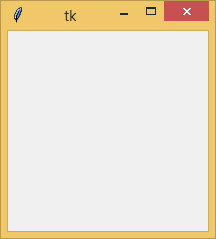
\includegraphics[scale=.6]{firstgui}\\
\end{figure}

Note that we have not created any widgets here.  We’ll come back to that later…

We can run our application as it it.   

Our first GUI Application doesn't do much:  it opens a window and waits…

To stop the program, we need to  close the window.

Before moving on to a more interesting application, let's take a closer look at each of the steps involved above:

\subsubsection{Importing tkinter}

Using 'import tkinter' to import the module implies that to access tkinter identifiers, we'll need to prefix them with tkinter.  So when we write tkinter.Tk(), we are instantiating an object of the Tk class; the Tk class is defined in the tkinter module. 

In a very large GUI application, this prefixing can get tedious and confusing.  In this case, it is OK to import everything into the application's namespace as follows:

\begin{lstlisting}
from tkinter import *
\end{lstlisting}

\subsubsection{Creating the main window}

\begin{lstlisting}
root = tkinter.Tk()
\end{lstlisting}

Here we have created a top level window for our application:  it is an \textit{instance} of the class tkinter.Tk.

By convention, the top level window is usually named root.  We should only create one root window for each program and it must be created before any other widgets. 

\subsubsection{Entering the Event Loop}

\begin{lstlisting}
root.mainloop()
\end{lstlisting}

Here we are invoking the mainloop method on the root object.

As the mainloop runs, it waits for events to happen. 

If an event occurs, it is handled by the corresponding handler if such a handler exists and the loop continues running, waiting for the next event. 

The loop continues to execute until the root window is closed.

One more thing - customizing our root window?

Notice that 'tk' that appears at the top of our application window?  That's the default title of a root tkinter window.  We can change it if we like by invoking the title method on the root window as shown below:

\begin{lstlisting}
# import the tkinter module - step 1

import tkinter

def main():

    # create the GUI application main window - step 2

    root = tkinter.Tk()

    #customize our GUI application main window - step 2a

    root.title('CS 21 A')

    # enter the main event loop and wait for events - step 4

    root.mainloop()

 

if __name__ == '__main__':

    main()
\end{lstlisting}

And here's what we get:
\begin{figure}[h]
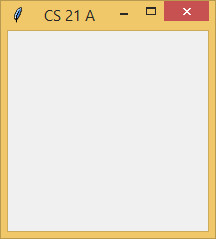
\includegraphics[scale=.6]{rootwtitle}\\
\end{figure}

\subsection{General GUI Design}
When we develop a GUI application, there are some general tasks that we need to accomplish:
\begin{itemize}
\item We need to specify what the application will look like: 
we do that by creating different visual components.  In tkinter, these components are called \textbf{widgets}.
\item We need to specify what the application will do: we do that by writing methods and functions that perform certain tasks.  These methods and functions are the event handlers, also called \textbf{callbacks}.
\item We need to \textbf{associate} (or bind) the looking with the doing: we do that by associating specific events on widgets with the event handlers we have written.
\item We need to write code that sits and waits for input from the user.  We've seen how to do that in the previous section.
We'll now go on to see how to achieve the first three subtasks above.
\end{itemize}

\subsection{Widgets}
We specify how we want a GUI to look by describing the widgets that we want it to display, and their spatial relationships (whether one widget is above or below, or to the right or left, of other widgets). 

Tkinter widgets include labels, frames, buttons, entries, menus, canvases and more.  We’ll cover some of the most useful ones.  

We can instantiate all widgets using the same general syntax:

WidgetClass(parent, option=value, ...)

This creates an instance of the WidgetClass, with the given parent, using the specified options.

All options have default values, so in the simplest case, we only have to specify the parent widget.  

Every widget has a parent widget.   However if we do not specify the parent,  tkinter uses the most recently created root window as the parent.

\subsection{The Label Widget}
Let's start by creating a \textit{Label widget}.

A Label widget can display text or an icon or some other image.  It is used to label other widgets. Unlike most other widgets, labels are not interactive.

A label widget is an instance of the Label class.  Following the general syntax for instantiating widgets, we can create a label as follows:

\begin{lstlisting}
my_label = tkinter.Label(parent, option, ...)
\end{lstlisting}

And here's a more specific example:

\begin{lstlisting}
# import the tkinter module
import tkinter


def main():
    # create the GUI application main window
    root = tkinter.Tk()
    # customize our GUI application main window
    root.title('CS 21 A')

    # instantiate a Label widget with root as the parent widget
    # use the text option to specify the text to display
    hello = tkinter.Label(root, text='Hello World!')

    # invoke the pack method on the widget
    hello.pack()

    # enter the main event loop and wait for events
    root.mainloop()


if __name__ == '__main__':
    main()
\end{lstlisting}

We run our program and we get our label:
 
And here's what we get:
\begin{figure}[h]
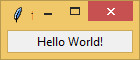
\includegraphics[scale=.6]{hellogui}\\
\end{figure}

Here again, to exit the program, we need to close the window.

\subsection{Parents and Packing}
Before moving on to other widgets, let's clarify some of the concepts introduced in the previous example.

\textbf{Parent}:  when we create a widget, we associate it with a parent.

The statement tkinter.Label(my{\_}parent) creates an instance of the Label class and associates that label instance with its parent.  The concept of parent is used in determining the lifetime of a widget.  When a parent component (such as the root) is closed, the parent knows who its children are, and can close them/destroy them before destroying itself.

\textbf{Packing}:  the pack method is invoked to ensure the widget is visible. If we don't pack a widget, we will not see it.  We could have used the grid (or the place) method instead.  We’ll come back to that later.

\subsection{The Frame Widget}
The Frame widget lets us group widgets. It works like a container, and it is responsible for arranging the position of other widgets.

It uses rectangular areas in the screen to organize the layout and to provide padding of these widgets. 

A frame widget is an instance of the Frame class:

\begin{lstlisting}
my_frame = tkinter.Frame(parent, option, ...)
\end{lstlisting}

Let's add two frames to our app: 

\begin{lstlisting}
# import the tkinter module
import tkinter


def main():
    # create the GUI application main window
    root = tkinter.Tk()
    # customize our GUI application main window
    root.title('CS 21 A')

    # instantiate a Label widget with root as the parent widget
    # use the text option to specify which text to display
    hello = tkinter.Label(root, text='Hello World!')

    # invoke the pack method on the widget to display it
    hello.pack()

    # we create a top frame
    top_frame = tkinter.Frame(root)
    top_frame.pack()

    # and a bottom frame
    bottom_frame = tkinter.Frame(root)
    # side is an optional parameter of the pack method.  It defaults to TOP.
    bottom_frame.pack(side=tkinter.BOTTOM)

    # enter the main event loop and wait for events
    root.mainloop()


if __name__ == '__main__':
    main()
\end{lstlisting}

Here we have created 2 frames.  When we run the program, the window looks exactly the same, nothing has changed.  The frames are empty containers.  

We'll see a more useful example of a frame widget in an upcoming section.

\subsection{The Button Widget}
The \textbf{Button widget} is used to add buttons in a GUI application. These buttons can display text or images.  They can also be 'clicked'.

We usually attach a function or a method to a button.  That function or method is then  called whenever the button is clicked.
 
A button widget is an instance of the Button class:
\begin{lstlisting}
my_button = tkinter.Button(parent, option, ...)
\end{lstlisting}

Buttons, like other widgets have a variety of options to control their size, their color, the text that they display, how their borders look, and so on.   Note that some options such as the background or foreground colors on buttons are NOT supported on Mac OS.

In this example, we will set just one option: the text.  

\begin{lstlisting}
# import the tkinter module
import tkinter


def main():
    # create the GUI application main window
    root = tkinter.Tk()
    # customize our GUI application main window
    root.title('CS 21 A')

    # instantiate a Label widget with root as the parent widget
    # use the text opetion to specify which text to display
    hello = tkinter.Label(root, text='Hello World!')

    # invoke the pack method on the widget
    hello.pack()

    # create a STOP button
    stop_button = tkinter.Button(root, text='STOP')
    stop_button.pack()

    # create a GO button
    go_button = tkinter.Button(root, text='GO')
    go_button.pack()

    # enter the main event loop and wait for events
    root.mainloop()


if __name__ == '__main__':
    main()
\end{lstlisting}

And here's the corresponding window on a Mac:
\begin{figure}[h]
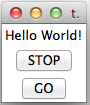
\includegraphics[]{MACbuttons}\\
\end{figure}

Note that unlike the labels, the buttons are clickable.

\subsection{The Canvas Widget}
The Canvas widget allows us to create a rectangular area intended for drawing pictures or other layouts. 

A canvas widget is an instance of the Canvas class:

\begin{lstlisting}
my_canvas = tkinter.Canvas(parent, option, ...)
\end{lstlisting}

Here's an example using the canvas widget.

\begin{lstlisting}
# import the tkinter module
import tkinter


def main():
    # create the GUI application main window
    root = tkinter.Tk()
    # create a label
    title = tkinter.Label(root, text="Let's Draw!")
    title.pack()

    # instantiate a Canvas widget with root as the parent widget
    canvas = tkinter.Canvas(root, background='green')

    # draw a blue rectangle on the canvas
    # create_rectangle returns an object id that we save in the variable body
    body = canvas.create_rectangle(50, 50, 150, 100, fill='blue')

    # draw two red circles on the canvas
    # create_oval also returns an object id
    wheel1 = canvas.create_oval(50, 100, 75, 125, fill='red')
    wheel2 = canvas.create_oval(125, 100, 150, 125, fill='red')

    canvas.pack()

    # enter the main event loop and wait for events
    root.mainloop()


if __name__ == '__main__':
    main()
\end{lstlisting}    

And here's what we get:
\begin{figure}[h]
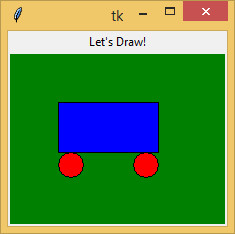
\includegraphics[scale=.6]{letsdraw}\\
\end{figure}


Let's take a closer look at the coordinate system used here.

The origin of the coordinate system is at the upper left corner, with the x coordinate increasing toward the right, and the y  coordinate increasing toward the bottom:

\begin{figure}[h]
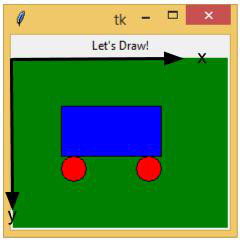
\includegraphics[scale=.6]{coordinates}\\
\end{figure}

The base unit is the pixel, with the top left pixel having coordinates (0,0). We can specify the coordinates as integers to denote pixels.  We  can also specify inches or centimeters as follows:

\begin{lstlisting}
rect = canvas.create_rectangle('1i','1i', '3i', '3i', fill='magenta')

rect = canvas.create_rectangle('1c','1c', '3c', '3c', fill='magenta')
\end{lstlisting}

To draw a rectangle we specify two points:  the top left corner and the bottom right corner.

 
\begin{lstlisting}
body = canvas.create_rectangle(50, 50, 150, 100, fill='blue')
\end{lstlisting}

50, 50 is the location of the top left corner 

150, 100 is the location of the pixel just outside of the bottom right corner.

All coordinates are relative to the canvas (not the root window.)

To draw an oval (or a circle) we fit it into a rectangle first and then we specify the top left corner and the bottom right corner of that rectangle.

We specify the corners of the enclosing rectangle

\begin{lstlisting}
 wheel1 = canvas.create_oval(50, 100, 75, 125, fill='red')
\end{lstlisting}

\begin{figure}[h]
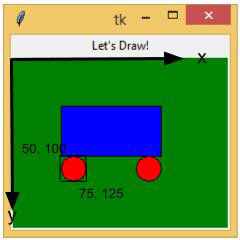
\includegraphics[scale=.6]{circlecoord}\\
\end{figure}

Similarly to draw a line on a canvas, we specify the coordinates of the endpoints:

\begin{lstlisting}
# import the tkinter module
import tkinter
 
def main():
 
    # create the GUI application main window
    root = tkinter.Tk()
    # create a label
    title = tkinter.Label(root, text="Let's Draw!")
    title.pack()
 
    # instantiate a Canvas widget with root as the parent widget
    canvas= tkinter.Canvas(root, background='green')
 
    # draw a line
    my_line = canvas.create_line(50, 50, 150, 200)
 
    canvas.pack()
 
    # enter the main event loop and wait for events
    root.mainloop()
 
if __name__ == '__main__':
    main()
\end{lstlisting}

\begin{figure}[h]
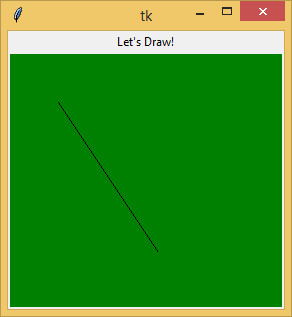
\includegraphics[scale=.6]{drawline}\\


\end{figure}

\subsection{Configuring Options}

The configure method may be used on any widget to add a new option or modify an existing option.

For example, for a canvas widget we can write:

\begin{lstlisting}
import tkinter
def main():
    root = tkinter.Tk()
    # create a green canvas first
    canvas = tkinter.Canvas(root, background='green')
    canvas.pack()
    # change the background color to yellow
    canvas.configure(background='yellow')
    root.mainloop()


if __name__ == '__main__':
    main()
\end{lstlisting} 

For a label widget, we can write:

\begin{lstlisting}
import tkinter
def main():
    root = tkinter.Tk()
    # create a label
    title = tkinter.Label(root, text="Let's Draw!")
    title.pack()
    # change the text
    title.configure(text='All Done!')
    # add a background color
    title.configure(background='red')
    root.mainloop()


if __name__ == '__main__':
    main()
\end{lstlisting}
 

\subsubsection{Configuring Canvas Object Options}
Similarly the \textit{itemconfigure} method may be used on a canvas widget to add a new option or modify an existing option of a canvas object such as a rectangle, oval or line.

\begin{lstlisting}
import tkinter

def main():
    # create the GUI application main window
    root = tkinter.Tk()
    # create a label
    title = tkinter.Label(root, text="Let's Draw!")
    title.pack()

    # instantiate a Canvas widget with root as the parent widget
    canvas = tkinter.Canvas(root, background='green')

    # draw a line
    my_line = canvas.create_line(50, 50, 150, 200)
    canvas.pack()
    # Add a color and a width to the line
    canvas.itemconfigure(my_line, fill='red', width=10)

    # enter the main event loop and wait for events
    root.mainloop()


if __name__ == '__main__':
    main()
\end{lstlisting}

\subsection{More Methods for Our Canvas}
There are some more useful methods defined on the canvas object.

The find{\_}all method returns a list containing all the objects currently found on the canvas.  The following code will change the fill color of all canvas objects to yellow: 

\begin{lstlisting}
for shape in canvas.find_all():


    canvas.itemconfigure(shape, fill='yellow')
\end{lstlisting}

The find{\_}closest returns a tuple containing the object that is the closest to a given point.  The following code will change the fill color of the shape closest to the top left corner (coordinates 0, 0) to purple.  Note that since the method returns a tuple, we use [0] to access the object:

\begin{lstlisting}
    top_left = canvas.find_closest(0, 0)[0]
    canvas.itemconfigure(top_left, fill='purple')
\end{lstlisting}

\subsection{Geometry Managers}
When we create a widget, it does not appear in the window until we register it with a geometry manager.

There are 3 geometry managers available in tkinter.  
\begin{itemize}
\item The \textit{pack} geometry manager  creates a layout by 'packing' the widgets into a parent widget,  treating them as rectangular blocks. 
\item The \textit{grid} geometry manager creates table-like layouts, organizing the widgets in a 2-dimensional grid. 
\item The \textit{place} geometry manager allows us to explicitly place a widget in a given position. It is seldom needed.
\end{itemize}

All widgets have the following methods corresponding to the 3 geometry managers:
\begin{itemize}
\item pack
\item grid
\item place
\end{itemize}

We 'register' a widget with a geometry manager by invoking one of the above methods on the widget.

We can use any of the geometry manager in a given window but we must not mix them in the same window.

The grid manager:

The grid manager treats every window or frame as a table of rows and columns.

The width of each column is the width of the widest cell in that column.

The height of each row is the height of the largest cell in that row.

The grid method takes two optional keyword arguments:  row and column.

The column argument allows us to specify the column number in the parent's grid where the widget will be placed.  Column numbers start at 0.   The column argument defaults to 0.

The row argument allows us to specify the row number in the parent's grid where the widget will be placed.  Row numbers start at 0.  The row argument defaults to the next available  row in the grid.

We'll illustrate the use of the grid geometry manager with a simple example.

\begin{lstlisting}
# import the tkinter module
import tkinter

# this is our color dictionary
COLORS = {'red': 'rouge', 'blue': 'bleu', 'green': 'vert',
          'yellow': 'jaune', 'black': 'noir', 'white': 'blanc'}


def main():
    # create the GUI application main window
    root = tkinter.Tk()

    # set the title for the window
    root.title("Colors")

    # add a label
    table_label = tkinter.Label(root, text="Color Review")

    # register it with a geometry manager
    table_label.grid()

    # instantiate a frame for our table
    table = tkinter.Frame(root)

    # register it with a geometry manager
    table.grid()

    row_count = 0
    # loop through the colors in our dictionary
    for color in COLORS:
        # instantiate a label for the English name
        color_english = tkinter.Label(table, text=color)
        # instantiate a label for the French name
        color_french = tkinter.Label(table, text=COLORS[color])
        # instantiate a label to show the color
        color_swatch = tkinter.Label(table, background=color, width=12)

        # each label goes in a different column - same row.
        color_english.grid(row=row_count, column=0)
        color_french.grid(row=row_count, column=1)
        color_swatch.grid(row=row_count, column=2)

        row_count += 1

    # enter the main event loop and wait for events
    root.mainloop()


if __name__ == '__main__':
    main()
\end{lstlisting}

And here's our window.  There are 6 rows and 3 columns in the table frame.
\begin{figure}[h]
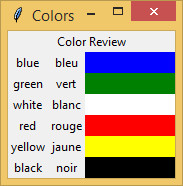
\includegraphics[scale=.6]{colorreview}
\end{figure}\\

Note that the placement of a widget is relative to the grid of the widget's parent.  So the placement of  table{\_}label ('Color Review') and the table frame is relative to the grid of the root window whereas the placement of the color{\_}english, color{\_}french and color{\_}swatch labels is relative to the grid of their parent, the table frame.

\subsection{Events and Handlers}
We have seen how to display various components in our GUI window but we have not seen how to capture the user input and initiate an action based on that input.

Several widgets accept user input and there are two ways to associate actions with events on widgets.

Some widgets such as buttons have a command option that lets us specify a function or a method, called a handler.  The handler will be called whenever the user clicks that button.  

Let's illustrate that option with a generic board game GUI with a START and QUIT buttons.  

\begin{lstlisting}
# -----------------------------------------------------------------------------
# Name:        game
# Purpose:     Implement a general board game
#
# Author:      Rula Khayrallah
# -----------------------------------------------------------------------------
'''
Module to implement a generic board GUI game app
'''
import tkinter


class Game(object):
    '''
    GUI Game class to support a general purpose 8 x 8 board game

    Argument:
    parent: (tkinter.Tk) the root window object

    Attributes:
    parent: (tkinter.Tk) the root window object
    canvas: (tkinter.Canvas) canvas representing the game board
    '''

    # we specify a class variable for the tile_size
    tile_size = 50

    def __init__(self, parent):
        parent.title('CS 21A Board Game')
        # save the parent in the object so that it can be accessed by draw_board
        self.parent = parent

        # create a START button and associate it with the start method
        start_button = tkinter.Button(self.parent, text='START',
                                      width=20,
                                      command=self.start)
        # register it with a geometry manager
        start_button.grid()

        # create a QUIT button and associate it with the quit method
        quit_button = tkinter.Button(self.parent, text='QUIT',
                                     width=20,
                                     command=self.quit)
        # register it with a geometry manager
        quit_button.grid()

        self.draw_board()

    def draw_board(self):
        '''Initialize the game board '''
        # create a canvas to draw our board
        self.canvas = tkinter.Canvas(self.parent,
                                     width=self.tile_size * 8,
                                     height=self.tile_size * 8)
        # register it with a geometry manager
        self.canvas.grid()

        # draw the tiles on the canvas
        for row in range(8):
            for column in range(8):
                if (row + column) % 2 == 0:
                    color = 'black'
                else:
                    color = 'red'
                self.canvas.create_rectangle(self.tile_size * column,
                                             self.tile_size * row,
                                             self.tile_size * (column + 1),
                                             self.tile_size * (row + 1),
                                             fill=color)

    def start(self):
        ''' this method is called when the START button is pressed'''
        print('starting the game')

    def quit(self):
        ''' this method is called when the QUIT button is pressed'''
        print('quitting the game')


def main():
    # create the GUI application main window
    root = tkinter.Tk()

    # instantiate our Game object
    my_game = Game(root)

    # enter the main event loop and wait for events
    root.mainloop()


if __name__ == '__main__':
    main()
\end{lstlisting}

And here's our game window:

\begin{figure}[h]

\includegraphics[scale=.6]{guiboard}
\end{figure}\
 
If we press on the START and QUIT buttons, we get the following output in the console:

starting the game

quitting the game

The command option does not allow us to pass any arguments to the function or method. That's one reason why using object oriented design is advantageous.  The method has at least access to the underlying object.
Binding is a more general mechanism that allows the application to respond to many more kinds of inputs: the press or release of any keyboard key or mouse button; movement of the mouse into, around, or out of a widget; and many other events.

For each widget, we bind functions and methods to events:  if an event matching the event description occurs in the widget, the given function or method is invoked.

The function or method (handler) is passed an event object that contains more details about the event.

The general syntax is:

\begin{lstlisting}
widget.bind(event, handler)
\end{lstlisting}

The process of binding involves three different entities: 

\begin{itemize}
\item a widget such as a button, a canvas, a frame
\item a type of event such as a click of the left mouse button, or a press of a certain key on the keyboard
\item an event handler which is a function or method
\end{itemize}

Note that if we no longer want a handler to respond to an event on a given widget, we can use unbind to remove the association:

\begin{lstlisting}
widget.unbind(event)
\end{lstlisting}

Here are some of the most common event types and their meaning.  We'll illustrate their use with a simple drawing application in the next section.

<Button-1> - The leftmost mouse button is pressed over the widget.  

<Button-2> - The middle mouse button is pressed over the widget.  <Button-2> also corresponds to the secondary click on the MAC trackpad. 

<Button-3> - The rightmost mouse button is pressed over the widget.

<Double-Button-1> - The leftmost mouse button is double clicked over the widget.  

<Double-Button-2> - The middle mouse button is double clicked over the widget.  

<Double-Button-3> - The rightmost mouse button is pressed over the widget.

<B1-Motion> - The mouse is moved, with the leftmost mouse button held down.

<B2-Motion> - The mouse is moved, with the middle mouse button held down.

<B3-Motion> - The mouse is moved, with the rightmost mouse button held down.

<ButtonRelease-1> The leftmost mouse button was released. 

<ButtonRelease-2> The middle mouse button was released. 

<ButtonRelease-3> The rightmost mouse button was released. 

<Enter> The mouse pointer entered the widget. It does NOT mean that the user pressed the Enter key.

<Leave> The mouse pointer left the widget.

Character Events:  most printable characters can be used as is to denote an event. 

a - The user typed an 'a'. 

\subsubsection{The Event Object}

The event handler receives one argument: the event object.

That event object is a Python object, with a number of attributes describing the event. Here are some of the event object attributes:

widget: the widget which generated this event.   This is a valid Tkinter widget instance, not a name.

x, y: the current mouse position, in pixels.

char: the character code (keyboard events only), as a string.

\subsection{A simple Drawing Application}
Let's create a simple drawing app to illustrate the bind method, event types and the use of the event object.

\begin{lstlisting}
# -----------------------------------------------------------------------------
# Name:        draw
# Purpose:     Implement a simple drawing application
#
# Author:      Rula Khayrallah
# -----------------------------------------------------------------------------
"""
Module to implement a simple drawing app
"""
import tkinter


class DrawApp(object):
    """
    class to support a simple drawing app

    Argument:
    parent: (tkinter.Tk) the root window object

    Attribute:
    canvas:  (tkinter.Canvas) our drawing canvas
    """

    def __init__(self, parent):
        parent.title('CS 21A Drawing App')
        # create the canvas
        # since we need to access the canvas widget from other methods,
        # we save it in the object as an instance variable: self.canvas
        self.canvas = tkinter.Canvas(parent, width=300, height=300)
        # register it with a geometry manager
        self.canvas.grid()
        # bind the leftmost button click to the draw_circle method
        self.canvas.bind("<Button-1>", self.draw_circle)
        # bind the leftmost button double click to the draw_square method
        self.canvas.bind("<Double-Button-1>", self.draw_square)

    def draw_circle(self, event):
        """ Draw a magenta circle centered at the click position"""
        self.canvas.create_oval(event.x - 10,
                                event.y - 10,
                                event.x + 10,
                                event.y + 10,
                                fill="magenta")

    def draw_square(self, event):
        """ Draw a cyan square at the click position"""
        self.canvas.create_rectangle(event.x - 10,
                                     event.y - 10,
                                     event.x + 10,
                                     event.y + 10,
                                     fill="cyan")


def main():
    # create the GUI application main window
    root = tkinter.Tk()

    # instantiate our drawing app object
    my_app = DrawApp(root)

    # enter the main event loop and wait for events
    root.mainloop()


if __name__ == '__main__':
    main()
\end{lstlisting}

And here's our drawing app.  Clicking or double clicking on the window results in a circle or a square drawn at the click position:

\begin{figure}[h]
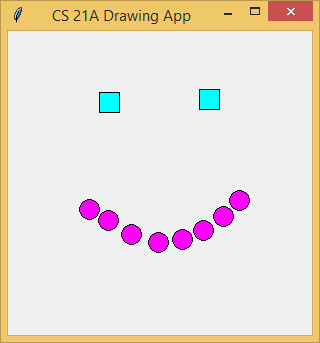
\includegraphics[scale=.6]{drawingclick}
\end{figure}\

Let's examine our binding statements and compare it to our bind syntax:

\begin{lstlisting}
widget.bind(event, handler)

self.canvas.bind("<Button-1>", self.draw_circle)
\end{lstlisting}

Here self.canvas is our widget, "<Button-1>" is our event and self.draw{\_}circle is our our handler.

self.canvas.bind("<Double-Button-1>", self.draw{\_}square)
Here self.canvas is our widget, "<Double-Button-1>" is our event and self.draw{\_}square is our our handler.

Note that we are binding different events to different handlers on the same widget.

Now let's examine one of our handlers:

\begin{lstlisting}
    def draw_circle(self, event):
        """ Draw a magenta circle centered at the click position"""
        self.canvas.create_oval(event.x - 10,
                                event.y - 10,
                                event.x + 10,
                                event.y + 10,
                                fill="magenta")
\end{lstlisting}

We note that the event object is automatically passed to the handler.  The handler has access to the coordinates of the event via the x and y attributes of the event object.

\subsection{A Simple Coloring Application}
Just for fun, here's another example of a simple coloring application:

\begin{lstlisting}
# -----------------------------------------------------------------------------
# Name:        paint
# Purpose:     A very simple coloring application
#
# Author:      Rula Khayrallah
# -----------------------------------------------------------------------------
"""
Module to implement a simple coloring app
"""
import tkinter

class PaintApp(object):
    """
    GUI PaintApp class for a simple coloring application.

    Argument:
    parent (tkinter.Tk): the root window object

    Attributes:
    canvas (tkinter.Canvas): the widget defining the area to be painted
    color (string): the paint color selected - red, green or blue
    """

    # Define a class variable for the default color to be used
    default_color = 'red'

    def __init__(self, parent):
        parent.title("CS 21A - Let's Paint!")

        # create a frame to group all the color buttons
        # this makes it easier to display them all in one row
        color_frame = tkinter.Frame(parent)
        # register it with a geometry manager
        color_frame.grid()
        # create a GREEN button and associate it with the green method
        # we save the button widgets in local variables since no other
        # method needs to access them
        green_button = tkinter.Button(color_frame, text='GREEN', width=10,
                                      command= self.green)
        # register it with a geometry manager
        green_button.grid(column=0, row=0)
        # create a GREEN button and associate it with the red method
        red_button = tkinter.Button(color_frame, text='RED', width=10,
                                    command= self.red)
        # register it with a geometry manager
        red_button.grid(column=1, row=0)
        # create a BLUE button and associate it with the blue method
        blue_button = tkinter.Button(color_frame, text='BLUE', width=10,
                                     command= self.blue)
        # register it with a geometry manager
        blue_button.grid(column=2, row=0)

        # instantiate our Canvas widget with the root as parent
        # since we need to access the canvas widget from the other methods
        # (play and erase), we save it in the object as an instance variable
        self.canvas= tkinter.Canvas(parent, width=300, height=300)

        # draw a rectangle on the canvas for the background
        self.canvas.create_rectangle(0, 0, 300, 300)

        # draw some shapes
        self.canvas.create_rectangle(50, 50, 150, 100)
        self.canvas.create_oval(50, 100, 75, 125)
        self.canvas.create_oval(125, 100, 150, 125)
        # a house
        self.canvas.create_rectangle(175, 150, 275, 250)
        # the roof is a triangle (polygon with 3 sides)
        self.canvas.create_polygon(165, 150, 225, 100, 285, 150,
                                   outline='black' )
        # a flower
        self.canvas.create_oval(50, 200, 75, 225)
        self.canvas.create_oval(50, 175, 75, 200)
        self.canvas.create_oval(50, 225, 75, 250)
        self.canvas.create_oval(25, 187, 50, 212)
        self.canvas.create_oval(25, 212, 50, 237)
        self.canvas.create_oval(75, 187, 100, 212)
        self.canvas.create_oval(75, 212, 100, 237)

        # register our canvas with a geometry manager
        self.canvas.grid()

        # when the user clicks on the canvas, we invoke self.paint
        self.canvas.bind("<Button-1>", self.paint)

        # create an ERASER button and associate it with the erase method
        erase_button = tkinter.Button(parent, text='ERASER', width=30,
                                      command= self.erase)
        # register it with a geometry manager
        erase_button.grid()
        # set the paint color to the default color
        self.color = self.default_color
        #fill all the shapes with a white color
        self.erase()



    def erase(self):
        """
        This method is invoked when the ERASE button is clicked.
        It fills all the shapes on the canvas with a white color.
        """
        for shape in self.canvas.find_all():
            self.canvas.itemconfigure(shape, fill='white')

    def green(self):
        """
        This method is invoked when the GREEN button is clicked.
        It sets the paint color to green.
        """
        self.color = "green"

    def red(self):
        """
        This method is invoked when the RED button is clicked.
        It sets the paint color to red.
        """
        self.color = "red"

    def blue(self):
        """
        This method is invoked when the BLUE button is clicked.
        It sets the paint color to blue.
        """
        self.color = "blue"

    def paint(self, event):
        """
        This method is invoked when the user clicks on the canvas
        It fills the enclosing shape with the paint color
        """
        shape = self.canvas.find_closest(event.x, event.y)
        self.canvas.itemconfigure(shape, fill=self.color)

def main():

    # create the GUI application main window
    root = tkinter.Tk()
    # Instantiate our painting app object
    my_game = PaintApp(root)
    # enter the main event loop and wait for events
    root.mainloop()

if __name__ == '__main__':
    main()
\end{lstlisting}

Here's the initial window that we get:

\begin{figure}[h]
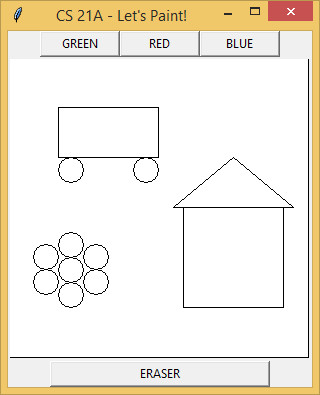
\includegraphics[scale=.6]{paint1}
\end{figure}\

And here's the window after we've done some coloring:

\begin{figure}[h]
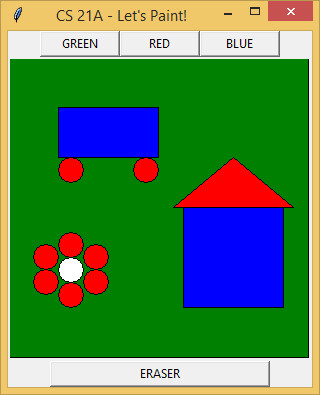
\includegraphics[scale=.6]{paint2}
\end{figure}\

\section{Assertions and Unit Testing}
\subsection{Assertions}
An assertion is a sanity-check that we can turn on when we are testing our program then turn  off when we are done testing.

Assertions are a convenient way to insert debugging statements into a program.

Assertions are carried out by the assert statement.

The syntax is as follows:

assert expression

Or:

assert expression,  description

If the assertion fails, Python raises an AssertionError.   AssertionError exceptions can be caught and handled like any other exception using the try-except statement.  If an assertion error is  not handled, it will terminate the program and produce a traceback.

Let's try a few assertions:

\begin{lstlisting}
>>> assert 1 + 1 == 2
\end{lstlisting}

The expression 1 + 1 == 2 is True, so the assert statement above does nothing.

\begin{lstlisting}
>>> assert 1 + 1 > 8

Traceback (most recent call last):
AssertionError
\end{lstlisting}

1 + 1 > 8 is False,  so the assert statement above raises an AssertionError.

We can also include a description that will only appear if the assertion fails.

\begin{lstlisting}
>>> assert 1 + 1 > 0, "this is the message that will appear if the assertion fails"

>>> assert 1 + 1 > 5, "this is the message that will appear if the assertion fails"

Traceback (most recent call last):
AssertionError: this is the message that will appear if the assertion fails
\end{lstlisting}
\subsubsection{Optimize Flags}

To speed up the loading of programs, Python caches a compiled byte code version of each module in the {\_}{\_}pycache{\_}{\_} directory under the name module.version.pyc.

We can use the -O or -OO options on the Python command to reduce the size of the compiled module. The -O flag removes assert statements, the -OO flag removes both assert statements and docstrings.   

Both flags also set the special builtin name {\_}{\_}debug{\_}{\_} to False.

A program does NOT run faster when it is optimized. The only thing that is faster is the speed with which it is loaded.

Let's take a look at an example:  the program below includes an assertion that will always be False.

\begin{lstlisting}
#-------------------------------------------------------------------------------
# Name:        asserttest.py
# Purpose:     test assert statements with the -O flag
#
# Author:      Rula Khayrallah
#-------------------------------------------------------------------------------
"""
Include an assertion that is always False
"""
 
def main():
    assert 0 > 1, 'this assertion is always False'
    print('Hello World!')
 
if __name__ == '__main__':
    main()
\end{lstlisting}

Now let's run the program without optimizing it from the terminal window:

\begin{lstlisting}
>python asserttest.py
Traceback (most recent call last):
  File "asserttest.py", line 16, in <module>
    main()
  File "asserttest.py", line 12, in main
    assert 0 > 1, 'this assertion is always False'
AssertionError: this assertion is always False
\end{lstlisting}

If we run the same program with the optimize flag, the assertion is ignored and we get:

\begin{lstlisting}
>python -O asserttest.py
Hello World!
\end{lstlisting}
 
\subsubsection{Assertions or Exceptions?}
A good guideline is to use an assertion to check for things that would only happen if there is a bug in our code.

An exception, on the other hand is used when we expect an error to happen and we need to handle it.

We can use an assertion at the start of a function to check for valid input (to the function, not user input) and after a function call to check for valid output.

Consider the following function that is supposed to compute a grade for a course based on the weights of several components.

\begin{lstlisting}
 def calculate_grade(homework, midterm, final):

    """ Compute the overall numeric grade for the course based on the weights"""

   #  we first assert that the input to our function is valid

    assert homework <= 100 and homework >= 0, "invalid grade"

    assert midterm <= 100 and midterm >= 0, "invalid grade"

    assert final <= 100 and final >= 0, "invalid grade"

    grade = (

            final * 0.5 +

            homework * 0.7 +

            midterm * 0.1

            )

   # we assert that our computation results in a valid grade

    assert grade <= 100 and grade >= 0, 'Invalid grade computation'

    return grade
\end{lstlisting}

The assertion may fail here because there is a bug in our code:  the weights for the various grades do not add up to 1 so we may end up with a grade > 100.

Assuming our function is defined in the module grades.py, we can write:

\begin{lstlisting}
>>> from grades import calculate_grade
>>> calculate_grade(95, 80, 95)
Traceback (most recent call last):
  File "<input>", line 1, in <module>
AssertionError: Invalid grade computation
\end{lstlisting}

On the other hand errors in user input are expected to occur even if our code is bug-free.  These errors are handled with exceptions not assertions.

\subsection{Unit Testing and TDD}
Unit testing is an important part of any software development strategy. 

It is important to write unit tests early and to keep them up to date as code and requirements change. 

Test Driven Development (TDD) advocates writing tests before writing  the code:  we write the test based on how we would like the code to behave, then we write the code that makes the test pass. This forces us to really understand the requirements before we start writing the code.

\subsection{The unittest Module}
The \textit{unittest} module is a  unit testing framework available in the Python Standard Library.

The unittest module supports test automation, sharing of setup and shutdown code for tests, aggregation of tests into collections, and independence of the tests from the reporting framework.

To create tests using the Python unit testing framework, we first have to import the module:

\begin{lstlisting}
import unittest 
\end{lstlisting}

To unit test methods or functions in a given module, we also have to be able to access them.

So in order to test the Car class methods for example, we need to import car.

So now we have:

\begin{lstlisting}
import unittest

import car
\end{lstlisting}

Now we can start writing our test cases.

\subsection{Test Cases and Test Fixtures}
A test case is an individual unit of testing. A test case checks for specific responses to a particular set of inputs.

The unittest module provides a base class, TestCase, which may be used to create new test cases.  Defining a test case involves defining a subclass of TestCase.

This is how we create a new test case to test the Car class.  Our test case class TestCar is a subclass of unittest.TestCase.

\begin{lstlisting}
class TestCar(unittest.TestCase):
 
    """
    Test case for the normal execution of Car methods
    """
\end{lstlisting}

Before we test a certain method, we may have to do some initial setup.

A test fixture represents the preparation needed to perform one or more tests, and any associated cleanup actions.

The unittest framework supports test fixtures with the setUp and tearDown methods.

When a setUp method is defined for a given test case, it is invoked prior to each test. 

Similarly, if a tearDown method is defined for a given test case, it is invoked after each test. 

Let's define our test fixture for the TestCar test case. We'll create three cars with different initial conditions.

\begin{lstlisting}
    def setUp(self):
        """
        Create three cars for testing.
        The first car has a fuel efficiency of 20 miles/gallon, initial
        mileage of 1000 miles and 9 gallons of fuel in the tank.
        The second car has a fuel efficiency of 30 miles/gallon, initial
        mileage of 5000 miles and 2 gallons of fuel in the tank
        The third car has a fuel efficiency of 24 miles/gallon, initial
        mileage of 0 miles and an empty gas tank.
        """
        self.first_car = car.Car('Porshe', '911', 20, 1000, 9)
        self.second_car = car.Car('Honda', 'Civic', 30, 2000, 2)
        self.third_car = car.Car('Honda', 'Pilot', 24)
\end{lstlisting}

Note that we save the three car objects as instance variables so that we can access them in the test methods.

Note also that to instantiate our Car class, we have to use its fully qualified name:  car.Car.

We will not define a tearDown method for our test case.

\subsection{Tests and Assertion Methods}
Within a test case, we define individual tests by defining methods whose names start with 'test'.

\begin{lstlisting}
def test_drive(self):

        """ test the drive method in the Car class"""  

def test_add_gas(self):

        """ test the add_gas method in the Car class"""  
\end{lstlisting}

Let's fill in the code for the methods above:

\begin{lstlisting}
    def test_drive(self):
        """ test the drive method in the Car class""" 
        # driving when there is enough gas in the tank
        self.first_car.drive(100)
        self.assertEqual(self.first_car.mileage, 1100)
        self.assertEqual(self.first_car.gas_in_tank, 4)
        # driving when there is not enough gas in the tank
        self.second_car.drive(200)
        self.assertEqual(self.second_car.gas_in_tank, 0)
        self.assertEqual(self.second_car.mileage, 2060)
        # driving when there is no gas in the tank
        self.third_car.drive(20)
        self.assertEqual(self.third_car.gas_in_tank, 0)
        self.assertEqual(self.third_car.mileage, 0)
\end{lstlisting}

This is our first test:  we are testing the drive method in the Car class.

We invoke the drive method on the three Car objects that we saved in our test case instance: self.first{\_}car, self.second{\_}car and self.third{\_}car.  This was done in the setUp method.

Given our fixture we know what the expected mileage and gas in tank for each car should be after the drive method is invoked.  

assertEqual is a method defined on the test case object.  The call to assertEqual is used to check for the expected result.  

If the result is NOT equal to the one we provided, an assertion exception is raised but is NOT reported on until the end of the tests.

\begin{lstlisting}
    def test_add_gas(self):
        """ test the add_gas method in the Car class""" 
        self.first_car.add_gas(3)
        self.assertEqual(self.first_car.gas_in_tank, 12)
        # the method returns a Car object
        self.assertIsInstance(self.second_car.add_gas(10), car.Car)
        self.third_car.add_gas(5)
        self.assertEqual(self.third_car.gas_in_tank, 5)
       # the mileage is not affected
        self.assertEqual(self.third_car.mileage, 0)
\end{lstlisting}

This is another test:  we are testing the add{\_}gas method in the Car class.

assertIsInstance is another method defined on the test case object.  The call to assertIsInstance is used to check that the object returned by the add{\_}gas method is an instance of the Car class.

The TestCase class provides a number of assertion methods to check for and report failures.

These methods are used instead of the assert statement so that all the test results can be accumulated and reported on at the end.

Here's a list of the assertion methods available:
\begin{itemize}
\item assertEqual
\item assertNotEqual
\item assertTrue
\item assertFalse
\item assertIs
\item assertIsNot
\item assertIsNone
\item assertIsNotNone
\item assertIn
\item assertNotIn
\item assertIsInstance
\item assertNotIsInstance
\end{itemize}

\subsection{Unit Testing Example}
This is how all the components fit together in the module testcar.py:

\begin{lstlisting}
# -----------------------------------------------------------------------------
# Name:        testcar.py
# Purpose:     demonstrate the use of the unittest module
# Author:      Rula Khayrallah
# -----------------------------------------------------------------------------
import unittest
import car


class TestCar(unittest.TestCase):
    """
    Test case for the normal execution of Car methods
    """

    def setUp(self):
        """
        Create three cars for testing.
        The first car has a fuel efficiency of 20 miles/gallon, initial
        mileage of 1000 miles and 9 gallons of fuel in the tank.
        The second car has a fuel efficiency of 30 miles/gallon, initial
        mileage of 5000 miles and 2 gallons of fuel in the tank
        The third car has a fuel efficiency of 24 miles/gallon, initial
        mileage of 0 miles and an empty gas tank.
        """
        self.first_car = car.Car('Porshe', '911', 20, 1000, 9)
        self.second_car = car.Car('Honda', 'Civic', 30, 2000, 2)
        self.third_car = car.Car('Honda', 'Pilot', 24)

    def test_drive(self):
        """ test the drive method in the Car class"""
        # driving when there is enough gas in the tank
        self.first_car.drive(100)
        self.assertEqual(self.first_car.mileage, 1100)
        self.assertEqual(self.first_car.gas_in_tank, 4)
        # driving when there is not enough gas in the tank
        self.second_car.drive(200)
        self.assertEqual(self.second_car.gas_in_tank, 0)
        self.assertEqual(self.second_car.mileage, 2060)
        # driving when there is no gas in the tank
        self.third_car.drive(20)
        self.assertEqual(self.third_car.gas_in_tank, 0)
        self.assertEqual(self.third_car.mileage, 0)

    def test_add_gas(self):
        """ test the add_gas method in the Car class"""
        self.first_car.add_gas(3)
        self.assertEqual(self.first_car.gas_in_tank, 12)
        # the method returns a Car object
        self.assertIsInstance(self.second_car.add_gas(10), car.Car)
        self.third_car.add_gas(5)
        self.assertEqual(self.third_car.gas_in_tank, 5)
        # the mileage is not affected
        self.assertEqual(self.third_car.mileage, 0)
\end{lstlisting}
 
And here's our car module from section 10.8:
\begin{lstlisting}
class Car(object):

    """
    Represent a car in  my virtual world.

    Arguments:
    make (string): car make.
    model (string): car model.
    fuel_efficiency (float): in miles per gallon.
    mileage (float, optional): current mileage on car in miles, defaults to 0.
    gas (float, optional): current gas in the tank in gallons, defaults to 0.

    Attributes:
    make (string): car make.
    model (string): car model.
    fuel_efficiency (float): in miles per gallon.
    mileage (float): current mileage on the car in miles.
    gas_in_tank (float): current gas in the tank in gallons.
    """

    def __init__(self,  make,  model, fuel_efficiency, mileage=0, gas=0):
        self.make = make
        self.model = model
        self.fuel_efficiency = fuel_efficiency
        self.mileage = mileage
        self.gas_in_tank = gas

    def add_gas(self, amount):
        """
        Add gas to the car.
        Parameter:
        amount (float): the amount of gas to be added in gallons.
        Return:
        the updated car object (Car).
        """
        self.gas_in_tank += amount
        return self

    def drive(self, distance):
        """
        Drive a car a given distance, if possible.
        If there is not enough gas, drive as much as possible.
        Parameter:
        distance (float):  the distance to be driven in miles.
        Return:
        the updated car object (Car)
        """
        max_distance = self.fuel_efficiency * self.gas_in_tank
        if distance <= max_distance:  # we can drive the distance
            self.mileage += distance
            self.gas_in_tank = (self.gas_in_tank - 
                                distance / self.fuel_efficiency)
        else:   # not enough gas
            self.mileage += max_distance  # drive as far as possible
            self.gas_in_tank = 0
        return self
\end{lstlisting}

\subsection{Running the Tests}
The test cases contained in the module testcar.py may be run from the command line (or terminal window) by invoking the unittest module and passing testcar  as its argument:

\begin{lstlisting}
>python -m unittest testcar

..
----------------------------------------------------------------------
Ran 2 tests in 0.000s
 
OK
\end{lstlisting}

The two dots above indicate that two tests were run and passed.

For more details, we can use the -v (verbose) flag:

\begin{lstlisting}
>python -m unittest -v testcar
 
test_add_gas (testcar.TestCar)
test the add_gas method in the Car class ... ok
test_drive (testcar.TestCar)
test the drive method in the Car class ... ok
--------------------------------------------------------------------
Ran 2 tests in 0.001s
OK
\end{lstlisting}

We can also invoke unittest in discovery mode:  this will run all the test cases found in modules whose names match a certain pattern, the default being test*:

\begin{lstlisting}
>python -m unittest

..
-------------------------------------------------------------------
Ran 2 tests in 0.001s
OK
\end{lstlisting}
 
We can also specify verbose in discovery mode:

\begin{lstlisting}
> python -m unittest -v
 
test_add_gas (testcar.TestCar)
test the add_gas method in the Car class ... ok
test_drive (testcar.TestCar)
test the drive method in the Car class ... ok
--------------------------------------------------------------------
Ran 2 tests in 0.002s
OK
\end{lstlisting}

Now suppose we introduce an error in our drive method so that the mileage is not updated when there is not enough gas.

\begin{lstlisting}
    def drive(self, distance):
        """
        Drive a car a given distance, if possible.
        If there is not enough gas, drive as much as possible.
        Parameter:
        distance (float):  the distance to be driven in miles.
        Return:
        the updated car object (Car)
        """
        max_distance = self.fuel_efficiency * self.gas_in_tank
        if distance <= max_distance:  # we can drive the distance
            self.mileage += distance
            self.gas_in_tank = (self.gas_in_tank - 
                                            distance / self.fuel_efficiency)
        else:   # not enough gas
            # comment the line below to introduce the error
            # self.mileage += max_distance  # drive as far as possible
            self.gas_in_tank = 0
        return self
\end{lstlisting}
 
When we run the tests now, we get a different output.
 
 \begin{lstlisting}
>python -m unittest testcar
 
.F
======================================================================
FAIL: test_drive (testcar.TestCar)
test the drive method in the Car class
----------------------------------------------------------------------
Traceback (most recent call last):
  File "C:\Users\Rula\Documents\CS21A\testcar.py", line 37, in test_drive
    self.assertEqual(self.second_car.mileage, 2060)
AssertionError: 2000 != 2060
 
----------------------------------------------------------------------
Ran 2 tests in 0.003s
 
FAILED (failures=1)
\end{lstlisting}

Note the .F above indicating that the first test passed and the second failed. 

We get more details in verbose mode:

\begin{lstlisting}
>python -m unittest -v
 
test_add_gas (testcar.TestCar)
test the add_gas method in the Car class ... ok
test_drive (testcar.TestCar)
test the drive method in the Car class ... FAIL
 
======================================================================
FAIL: test_drive (testcar.TestCar)
test the drive method in the Car class
----------------------------------------------------------------------
Traceback (most recent call last):
  File "C:\Users\Rula\Documents\CS21A\testcar.py", line 37, in test_drive
    self.assertEqual(self.second_car.mileage, 2060)
AssertionError: 2000 != 2060
 
----------------------------------------------------------------------
Ran 2 tests in 0.002s
 
FAILED (failures=1)
\end{lstlisting}

\subsection{Example - Testing Functions}
Our goal is to write a unit test to test a function is{\_}passing defined inside a module named grading.py.

\begin{lstlisting}
# -----------------------------------------------------------------------------
# Name:        grading.py
# Purpose:     miscellaneous functions used for grading
# Author:      Rula Khayrallah
# -----------------------------------------------------------------------------
"""
Module that contains various grading functions
"""
PASSING_GRADE = 70  # minimum grade required to pass a course
 
def is_passing(grade):
    """
    Parameter: grade (float) a numeric grade between 0 and 100 inclusive
    Return: boolean - True if the grade is passing and False otherwise
    """
    return grade >= PASSING_GRADE
\end{lstlisting}
 
We create the following module testgrading.py to achieve our task:
 
 \begin{lstlisting}
# -----------------------------------------------------------------------------
# Name:        testgrading.py
# Purpose:     test various grading functions
# Author:      Rula Khayrallah
# -----------------------------------------------------------------------------
import unittest
import grading
 
class TestGrading(unittest.TestCase):
    """
    Test case for the normal execution of grading functions
    """
 
    def test_is_passing(self):
        """ test the is_passing function in the grading module"""
       # test a passing grade
        self.assertTrue(grading.is_passing(85))
       # test a failing grade
        self.assertFalse(grading.is_passing(68))
       # test a borderline passing grade and specify a message
        self.assertTrue(grading.is_passing(70),
                'Borderline grade not identified as passing')
\end{lstlisting}

Our test case did not include any fixtures:  we did not define any setUp or tearDown methods.

We used the assertTrue and assertFalse methods to check our results.  The assertion methods take an optional message that is displayed if the assertion fails.

We can run our test as follows:

\begin{lstlisting}
>python -m unittest -v testgrading
 
test_is_passing (testgrading.TestGrading)
test the is_passing function in the grading module ... ok
 
----------------------------------------------------------------------
Ran 1 test in 0.001s
 
OK
\end{lstlisting}
 
Let's introduce a bug in the function is{\_}passing by changing the >= sign to > :
\begin{lstlisting}
def is_passing(grade):
    """
    Parameter: grade (float) a numeric grade between 0 and 100 inclusive
    Return: boolean - True if the grade is passing and False otherwise
    """
    return grade > PASSING_GRADE
\end{lstlisting}

Running the test now results in the following:
 
 \begin{lstlisting}
>python -m unittest -v testgrading
 
test_is_passing (testgrading.TestGrading)
test the is_passing function in the grading module ... FAIL
 
======================================================================
FAIL: test_is_passing (testgrading.TestGrading)
test the is_passing function in the grading module
----------------------------------------------------------------------
Traceback (most recent call last):
  File "C:\Users\Rula\Documents\January CS 21A\testgrading.py", line 19, in test_is_passing
    'Borderline grade not identified as passing')
AssertionError: False is not true : Borderline grade not identified as passing
 
----------------------------------------------------------------------
Ran 1 test in 0.001s
 
FAILED (failures=1)
\end{lstlisting}

\section{More on Functions}
\subsection{Variable Number of Arguments}
We have already seen how to call a function or method using default arguments.

A default argument is an argument that assumes a default value if a value is not provided in the function call.  That default value is specified in the function or method definition.  The only restriction is that non-default parameters appear before default parameters in the function definition. 

\begin{lstlisting}
def diff(a, b=0):  
    return a - b 
\end{lstlisting}
     
When we provide a default value for b, we can call the function with two arguments:

\begin{lstlisting}
>>> diff (4, 2)
\end{lstlisting}

2

Or with just one argument:

\begin{lstlisting}
>>> diff (4 )

4
\end{lstlisting}

Note that the same rules apply to method arguments and class instantiations:

\begin{lstlisting}
class Car(object):

    def __init__(self,  make,  model, fuel_efficiency, mileage=0, gas=0):

>>> from car import Car
\end{lstlisting}

We can instantiate a Car object by specifying 5 arguments:

\begin{lstlisting}
>>> my_car = Car('Honda',  'Civic', 25,  10000, 12 )
\end{lstlisting}

Or just 4:
\begin{lstlisting}
>>> my_car = Car('Honda',  'Civic', 25,  10000)
\end{lstlisting}

Or just 3 arguments:

\begin{lstlisting}
>>> my_car = Car('Honda', 'Civic', 25 )
\end{lstlisting}

The unspecified arguments are then assigned the default value.

Sometimes we don't know beforehand how many arguments will be passed to the function by the user and we don't have any default values.

We have the option to specify that a function be called with an arbitrary number of arguments. The function will receive these arguments in a tuple. Before these variable arguments, zero or more normal arguments may occur.

To specify a variable number of argument, we use *args in the function definition.

We can also use *any{\_}other{\_}name instead of *args.

Here's an example:

\begin{lstlisting}
def test_args(req1, req2, *args):
    """this function takes at least two arguments"""
    print('first required argument', req1)
    print('second required argument', req2)
    for arg in args:
        print ('another argument', arg)
>>> test_args ('first', 'second', 'third', 'fourth')


first required argument first

second required argument second

another argument third

another argument fourth

>>> test_args ('first', 'second')

first required argument first

second required argument second

>>> test_args ('first')

Traceback (most recent call last):

TypeError: test_args() missing 1 required positional argument: 'req2'
\end{lstlisting}

And here's a more useful example:

\begin{lstlisting}
def product(*args):
    """
    return the product of the arguments provided or 1 if no argument is provided
    """"
    result = 1
    for number in args:
        result = result * number
    return result      
>>> product(2, 3, 4, 5)

120

>>> product(5)

5

>>> product (2, 3)

6

>>> product()

1
\end{lstlisting}

\subsubsection{Variable Keyword Arguments}

We can also define a function or a method so that it accepts an arbitrary number of keyword arguments.  The keywords do not have to be defined beforehand.

In the function or method definition we specify a final formal parameter of the form **kwargs. We can also use **any{\_}other{\_}name instead of **kwargs.

The function then receives a dictionary containing all keyword arguments except those corresponding to a formal parameter or *args.

*args, if present,  must occur before **kwargs.

Let's first write a trivial function that simply prints the keyword arguments dictionary:

\begin{lstlisting}
def test_kwargs(**kwargs):
    """this function prints the keyword arguments"""
    print (kwargs)
\end{lstlisting}
 
We can call the function with any keyword arguments we choose and with any number of keyword arguments:
 
\begin{lstlisting}
>>> test_kwargs(course='cs21A', grade=100)
{'grade': 100, 'course': 'cs21A'}

test_kwargs(name='Alice')

{'name': 'Alice'}
\end{lstlisting}

Here's a more useful example:

\begin{lstlisting}
def custom_print(name, **kwargs):
    """this function takes at least one argument"""
    print (name)
    for key in kwargs:
        print (key + ':', kwargs[key])
>>> custom_print('Alice', major='CS', email='alice@foothill.edu')

Alice

major: CS

email: alice@foothill.edu

>>> custom_print('Bob', phone='555-3743')

Bob

phone: 555-3743

>>> custom_print('Charlie')

Charlie

>>> custom_print()

Traceback (most recent call last):

TypeError: custom_print() missing 1 required positional argument: 'name'
\end{lstlisting}

\section{More Python Modules}
\subsection{The OS Module}
The OS module is another module included in the Python standard library.

It offers a platform independent way to access and manipulate local directories, files and environment variables.   It has a consistent interface across supported operating systems so our programs can run unchanged on any platform.

We have already seen how to use the  os.getcwd function to figure out what our working directory is.

On Windows, from the PyCharm console, we can type the following:

\begin{lstlisting}
>>> import os

>>> os.getcwd()

'C:\\Users\\Rula\\Documents\\CS21A'
\end{lstlisting}

We get the backslashes here because this example is on Windows.   One backslash shows as a double backslash because of the escaping issue with strings.

On a Mac, we get the following:

\begin{lstlisting}
>>> import os

>>> os.getcwd()

'/Users/rulakhayrallah/PycharmProjects/CS21A'
\end{lstlisting}

When we specify a filename with a relative path,  that relative path will start from our working directory.  The os.chdir function lets us change the current working directory.

On Windows:

\begin{lstlisting}
>>> import os

>>> os.getcwd()

'C:\\Users\\Rula\\Documents\\CS21A'

>>> os.chdir('/users')

>>> os.getcwd()

'C:\\users'

>>> os.chdir('Rula')

>>> os.getcwd()

'C:\\users\\Rula'

>>> os.chdir('Documents/CS21A')

>>> os.getcwd()

'C:\\users\\Rula\\Documents\\CS21A'
\end{lstlisting}

With all the os functions, we can use forward slashes across all the platforms (even on Windows.)

If we run this example on Mac OS X, we get the following. 

\begin{lstlisting}
>>> import os

>>> os.getcwd()

'/Users/rulakhayrallah/PycharmProjects/CS21A'

>>> os.chdir('/users')

>>> os.getcwd()

'/Users'

>>> os.chdir('rulakhayrallah')

>>> os.getcwd()

'/Users/rulakhayrallah'

>>> os.chdir('PycharmProjects/CS21A')

>>> os.getcwd()

'/Users/rulakhayrallah/PycharmProjects/CS21A'
\end{lstlisting}

os.sep will show us the character used to separate pathname components on our system.

On Windows:

\begin{lstlisting}
>>> os.sep

'\\'
\end{lstlisting}

On a Mac:

\begin{lstlisting}
>>> os.sep

'/'
\end{lstlisting}

The os.listdir function returns a list containing the names of the entries in a given directory.   The list is in arbitrary order.

If no argument is provided, the default '.' (current directory is used).

\begin{lstlisting}
>>> os.listdir()  

['.idea', 'car.py', 'crawled.txt', 'crawler.py', 'grader.py', 'helloagain.py', 'house.py', '__pycache__']

>>> os.listdir('C:/Users/Rula/Documents/CS 21A') 

['CS21A Syllabus.docx', 'CS21A Syllabus.pdf', 'Lectures', 'Programming Assignments', 'Python Programs', 'screencasts']
\end{lstlisting}

Files and subfolders are included in the list.

getcwd, chdir, listdir as well as sep are all in the os namespace.   We type os.getcwd, os.chdir, os.listdir and os.sep to access them.

Next we’ll see a number of functions that are in the os.path namespace.  os.path is a submodule of os.  We don’t need to import it separately if we have already imported os.

The os.path submodule includes the following functions:  os.path.join, os.path.split, os.path.splitext, os.path.realpath, os.path.exists and os.path.isfile.

\subsubsection{os.path.join()}

The os.path.join function intelligently constructs a pathname out of one or more partial pathnames. 

If any component is an absolute path, all previous components are thrown away, and joining continues from there on.

The function adds exactly one separator following each non-empty part except the last. 

Here's an example on Windows:

\begin{lstlisting}
>>> os.path.join('users/rula/documents', 'cs21a', 'tests')

'users/rula/documents\\cs21a\\tests'
\end{lstlisting}

If any component is an absolute path, all previous components are thrown away:

\begin{lstlisting}
>>> os.path.join('users/rula/documents', 'c:/users/tests')

'c:/users/tests'

>>> os.path.join('users/rula/documents', 'cs21a', 'tests', 'crawled.txt')

'users/rula/documents\\cs21a\\tests\\crawled.txt'
\end{lstlisting}

Here's a similar example on a Mac:

\begin{lstlisting}
>>> os.path.join('users/rulakhayrallah', 'cs21a', 'tests')

'users/rulakhayrallah/cs21a/tests'
\end{lstlisting}

If any component is an absolute path, all previous components are thrown away:

\begin{lstlisting}
>>> os.path.join('users/rulakhayrallah', '/users/guest/test')

'/users/guest/test'

>>> os.path.join('users/rulakhayrallah/documents', 'cs21a', 'tests', 'crawled.txt')

'users/rulakhayrallah/documents/cs21a/tests/crawled.txt'
\end{lstlisting}

\subsubsection{os.path.split()}

The os.path.split function splits a full pathname and returns a tuple containing the path and filename. We can then use tuple unpacking to get each of the separate variables.

\begin{lstlisting}
>>> os.path.split('/users/rula/Documents/CS21A/hello.py')

('/users/rula/Documents/CS21A', 'hello.py')
\end{lstlisting}

We can also write, using tuple unpacking:

\begin{lstlisting}
>>> (pathname, filename) = os.path.split('/users/rula/Documents/CS21A/hello.py')

>>> pathname

'/users/rula/Documents/CS21A'

>>> filename

'hello.py'
\end{lstlisting}

Note that the file name may be empty:

\begin{lstlisting}
>>> pathname, filename = os.path.split('users/Rula/')

>>> pathname

'users/Rula'

>>> filename

' '
\end{lstlisting}

However, if we omit the / at the end:

\begin{lstlisting}
>>> pathname, filename = os.path.split('users/Rula')

>>> pathname

'users'

>>> filename

'Rula'
\end{lstlisting}

\subsubsection{os.path.splitext()}


The os.path.splitext function (ext for extension not text) splits a filename and returns a tuple containing the filename and the file extension. We can then use tuple unpacking to get each of the separate variables.
\begin{lstlisting}
>>> filename, ext = os.path.splitext ('users/Rula/CS21A/hello.py')

>>> filename

'users/Rula/CS21A/hello'

>>> ext

'.py'

>>> filename, ext = os.path.splitext ('hello.py')

>>> filename

'hello'

>>> ext

'.py'
\end{lstlisting}

The period separator is included in the extension here.

Here again, the extension may be empty.  

\begin{lstlisting}
>>> filename, ext = os.path.splitext ('hello')

>>> filename

'hello'

>>> ext

''
\end{lstlisting}

\subsubsection{os.path.realpath()}

The os.path.realpath function returns the absolute path of the specified filename, eliminating any symbolic links encountered in the path. 

Here's an example on Windows:

\begin{lstlisting}
>>> os.getcwd()

'C:\\users\\Rula\\Documents\\CS21A'

>>> os.path.realpath('hello.py')

'C:\\users\\Rula\\Documents\\CS21A\\hello.py' 

>>> os.path.realpath('/test/hello.py')

'C:\\test\\hello.py' 

>>> os.path.realpath('test/hello.py')

'C:\\users\\Rula\\Documents\\CS21A\\test\\hello.py'

>>> os.path.realpath('../hello.py')

'C:\\users\\Rula\\Documents\\hello.py'

>>> os.path.realpath('../../hello.py')

'C:\\users\\Rula\\hello.py'

>>> os.path.realpath('./test/hello.py')

'C:\\users\\Rula\\Documents\\CS21A\\test\\hello.py'
\end{lstlisting}

And a similar example on a Mac:

\begin{lstlisting}
>>> os.getcwd()

'/Users/rulakhayrallah/PycharmProjects/CS21A'

>>> os.path.realpath('hello.py')

'/Users/rulakhayrallah/PycharmProjects/CS21A/hello.py'

>>> os.path.realpath('/test/hello.py')

'/test/hello.py'

>>> os.path.realpath('test/hello.py')

'/Users/rulakhayrallah/PycharmProjects/CS21A/test/hello.py'

>>> os.path.realpath('../hello.py')

'/Users/rulakhayrallah/PycharmProjects/hello.py'

>>> os.path.realpath('../../hello.py')

'/Users/rulakhayrallah/hello.py'

>>> os.path.realpath('./test/hello.py')

'/Users/rulakhayrallah/PycharmProjects/CS21A/test/hello.py'
\end{lstlisting}

\subsubsection{No Guarantee of Existence}
Note that the path functions that we have seen so far (join, split, splitext and realpath) can be used to parse strings representing filenames into their component parts and to assemble components into absolute paths.

It is important to realize that these functions do not depend on the paths actually existing; they operate only on the strings.

What if we need to verify that a path or a file exists?

os.path.exists(path) returns True if the path exists.   It works for both files and directories.

os.path.isfile(path) returns True if the specified path  is an existing  file.   It returns False if the path is a directory.
\begin{lstlisting}
>>> os.path.exists('/users/Rula')

True

>>> os.path.isfile('/users/Rula')

False

>>> os.path.exists('hello.py')

True

>>> os.path.isfile('hello.py')

True

>>> os.path.isfile('nofile.py')

False
\end{lstlisting}

\subsection{Copy and Deep Copy}
Remember our discussion about variables 'referring' to objects as opposed to 'containing' them?

We have seen that an assignment statement on lists does not make a copy. Instead, the assignment makes the two variables point to the same list in memory.

\begin{lstlisting}
>>> alice = [98, 87,100]The two variables alice and bob point to the same location in memory

>>> bob = alice

>>> alice

[98, 87, 100] 

>>>  bob

[98, 87, 100]
\end{lstlisting}

What happens if we now change one list item in alice? 

\begin{lstlisting}
>>>  alice[1] = 0bob is changed too.

>>> alice                               

[98, 0, 100]                         

>>>  bob 

[98, 0, 100]
\end{lstlisting}

What if we wanted bob to have a different copy of the list, one that initially has the same values as alice but that is not affected by future changes to alice.

If the list we are copying is not nested, the following slice assignment will work.

\begin{lstlisting}
>>> alice = [98, 0, 100]one list pointed to by alice

>>>bob = alice[:]                          

>>> boband another list pointed to by bob

[98, 0, 100]

>>>  alice

[98, 0, 100]

>>> alice[1] = 5

>>>  alice

[98, 5, 100]

>>>  bob

[98, 0, 100]
\end{lstlisting}

However with nested lists the slice assignment will NOT work.  It is a shallow copy.

\begin{lstlisting}
>>> charlie = [100, 98, [85, 90], 85]

>>> diana = charlie[:]shallow copy

>>> diana

[100, 98, [85, 90], 85]

>>> charlie[1] = 0

>>> charlie

[100, 0, [85, 90], 85]

>>> diana

[100, 98, [85, 90], 85]

>>> charlie[2][1] = 0

>>> charlie

[100, 0, [85, 0], 85]

>>> diana

[100, 98, [85, 0], 85]
\end{lstlisting}

\subsubsection{The copy module}
The shallow versus deep copy issue is relevant not just for lists but for compound objects in general.

The copy module offers an alternative to deal with it.  It has 2 distinct functions:

\begin{itemize}
\item copy.copy()

\item copy.deepcopy()
\end{itemize}

The copy.copy() function  constructs a new compound object and then (to the extent possible) inserts references into it to the objects found in the original.

For lists, copy.copy() is equivalent to the slice copy.

The copy.deepcopy() function constructs a new compound object and then, recursively, inserts copies into it of the objects found in the original.

A deep copy duplicates the compound object as well as the contents of all of its contained objects.

Here's a copy and deepcopy list example:

\begin{lstlisting}
>>>import copy

>>> charlie = [100, 98, [85, 90], 85]copy vs deepcopy with lists

>>> diana = copy.copy(charlie)

>>> frank = copy.deepcopy(charlie)

>>> charlie[1] = 0

>>> charlie

[100, 0, [85, 90], 85]

>>> diana

[100, 98, [85, 90], 85]

>>> frank

[100, 98, [85, 90], 85]

>>> charlie[2][1] = 0

>>> charlie

[100, 0, [85, 0], 85]

>>> diana

[100, 98, [85, 0], 85]

>>> frank

[100, 98, [85, 90], 85]
\end{lstlisting}

And here's a compound object example:

\begin{lstlisting}
class Profile(object):
    """
    Represent a person's social profile
 
    Argument:
    name (string): a person's name - assumed to uniquely identify a person
 
    Attributes:
    name (string): a person's name - assumed to uniquely identify a person
    statuses (list): a list containing a person's statuses
    friends (set): set of friends for the given person.
                   it is the set of profile objects representing these friends.
    """
 
    def __init__(self,  name):
        self.name = name
        self.statuses = []
        self.friends = set()
>>> from social import Profile

>>> import copy

>>> alice = Profile('Alice')

>>> bob = Profile('Bob')

>>> charlie = Profile('Charlie')

>>> alice.add_friend(bob)

>>> copy_alice = copy.copy(alice)

>>> deepcopy_alice = copy.deepcopy(alice)

>>> alice.get_friends()

['Bob']

>>> copy_alice.get_friends()

['Bob']

>>> deepcopy_alice.get_friends()

['Bob']

>>> alice.add_friend(charlie)

>>> alice.get_friends()

['Bob', 'Charlie']

>>> copy_alice.get_friends()

['Bob', 'Charlie']

>>> deepcopy.get_friends()

['Bob']

Deepcopy and Object Identity:

>>> copy_alice is alice

False

>>> deepcopy_alice is alice

False

>>> copy_alice.friends is alice.friends

True

>>> deepcopy_alice.friends is alice.friends

False
\end{lstlisting}

\end{document}